% Beamer Presentation and Lecture Note Template
% Version 0.1
% by Paul Vesey

\mode<presentation> {
\usetheme{Antibes}
\setbeamercovered{invisible}
\setbeamertemplate{footline}[frame number]
\setbeamertemplate{navigation symbols}{} 
}

\usepackage{eurosym}
\usepackage{graphicx}
\usepackage{wasysym}
\usepackage{hyperref}
\usepackage{amsmath}
\usepackage{amssymb}
\usepackage{mathtools}
\usepackage{tikz}
\usepackage{pgf}
\usepackage{pgfplots}
\usepackage{pxfonts}
\usepackage{textcomp}
\usepackage{verbatim}
\usepackage{color}
\usepackage{xcolor}
\usepackage{fix-cm}


\author{Paul Vesey}
\institute[TUS]
{
Technological University of the Shannon \\
\medskip
{\emph{paul.vesey@tus.ie}}
}
\date{Autumn 2022}




\title[Project Management \& BIM]{Project Time Management}


\begin{document}
%
\usetikzlibrary{arrows}
\usepgflibrary{patterns}



\section{Project Time Management}



\tableofcontents
\newpage



\begin{frame}
\titlepage
\end{frame}
\begin{center}\line(1,0){250}\end{center}
%
%

\section{Project Scheduling Basics}


\begin{frame}
\begin{figure}
	\centering
		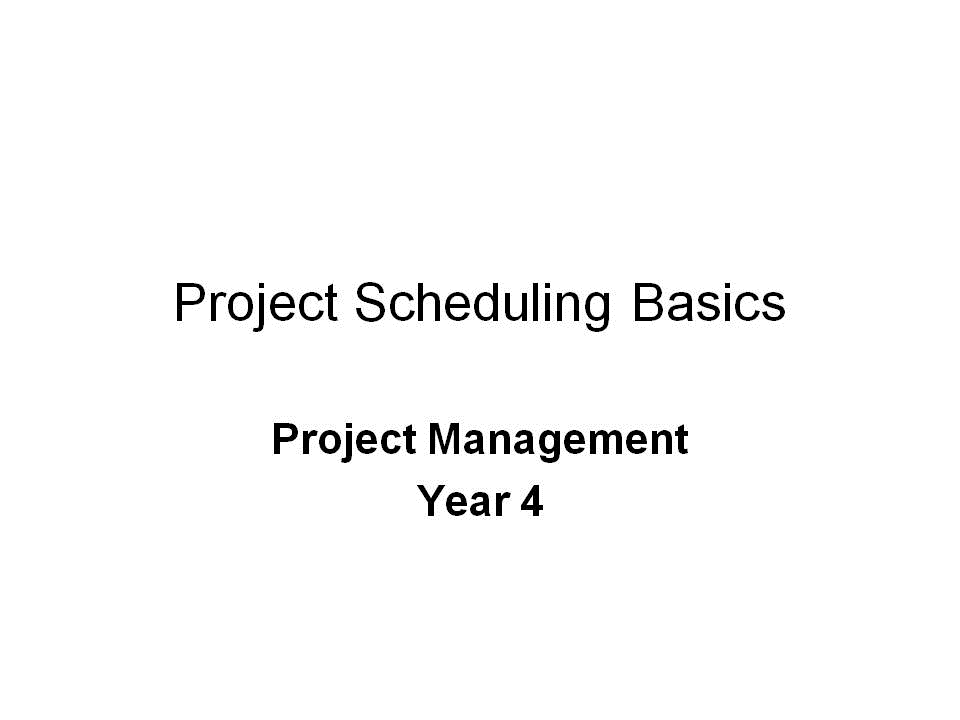
\includegraphics[width = 10.5cm]{oldnotes/Slide32.jpg}
\end{figure}
\end{frame}
\begin{center}\line(1,0){250}\end{center}



\begin{frame}
\begin{figure}
	\centering
		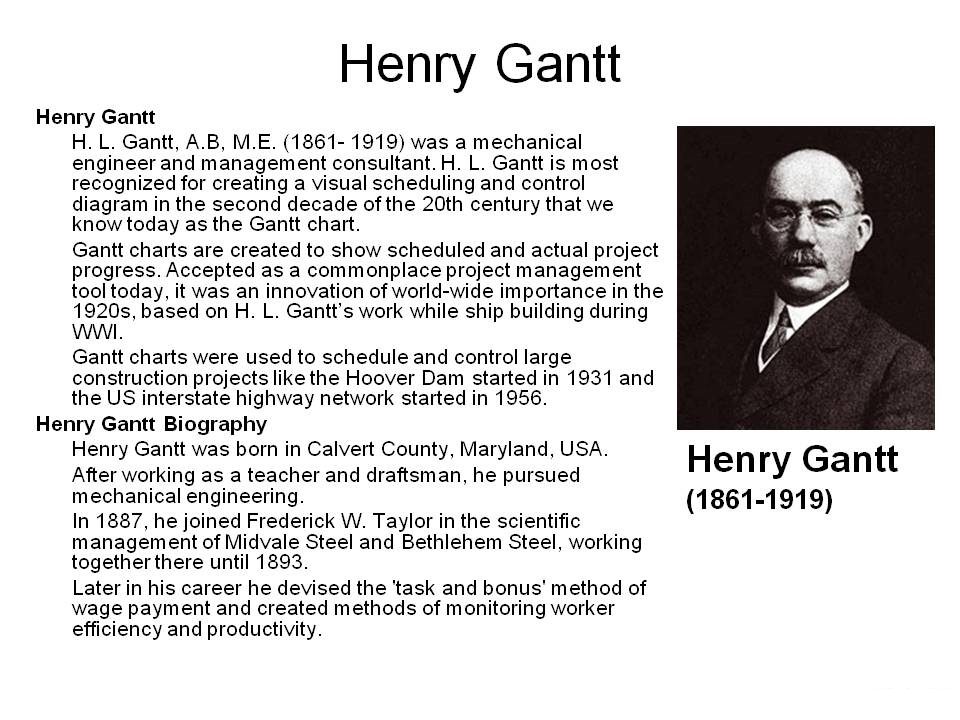
\includegraphics[width = 10.5cm]{oldnotes/Slide33.jpg}
\end{figure}
\end{frame}
\begin{center}\line(1,0){250}\end{center}





\begin{frame}
\begin{figure}
	\centering
		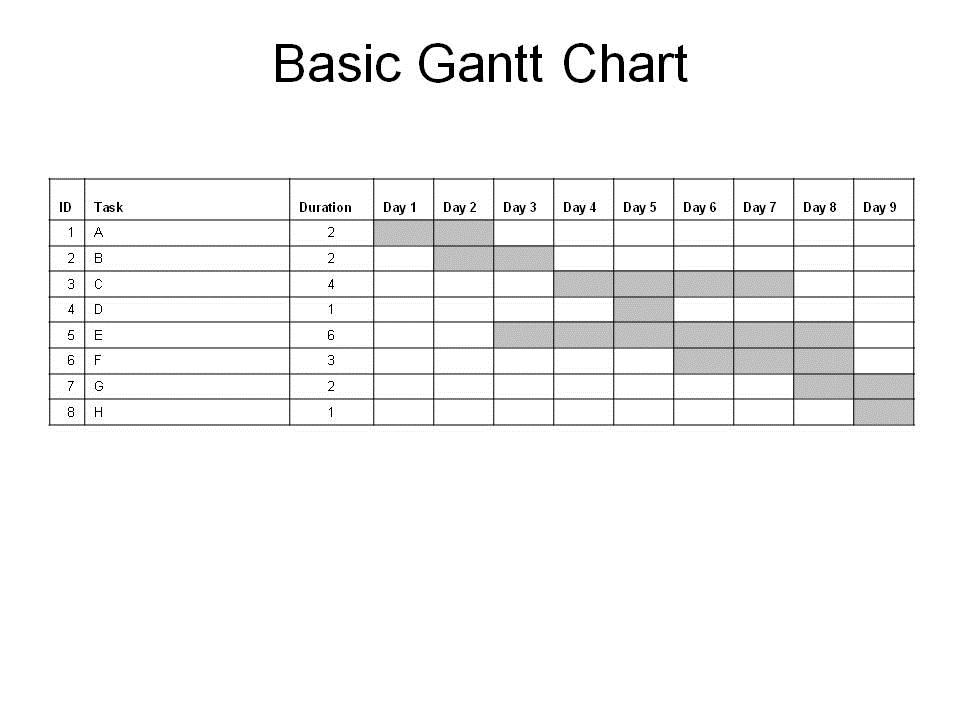
\includegraphics[width = 10.5cm]{oldnotes/Slide34.jpg}
\end{figure}
\end{frame}
\begin{center}\line(1,0){250}\end{center}





\begin{frame}
\begin{figure}
	\centering
		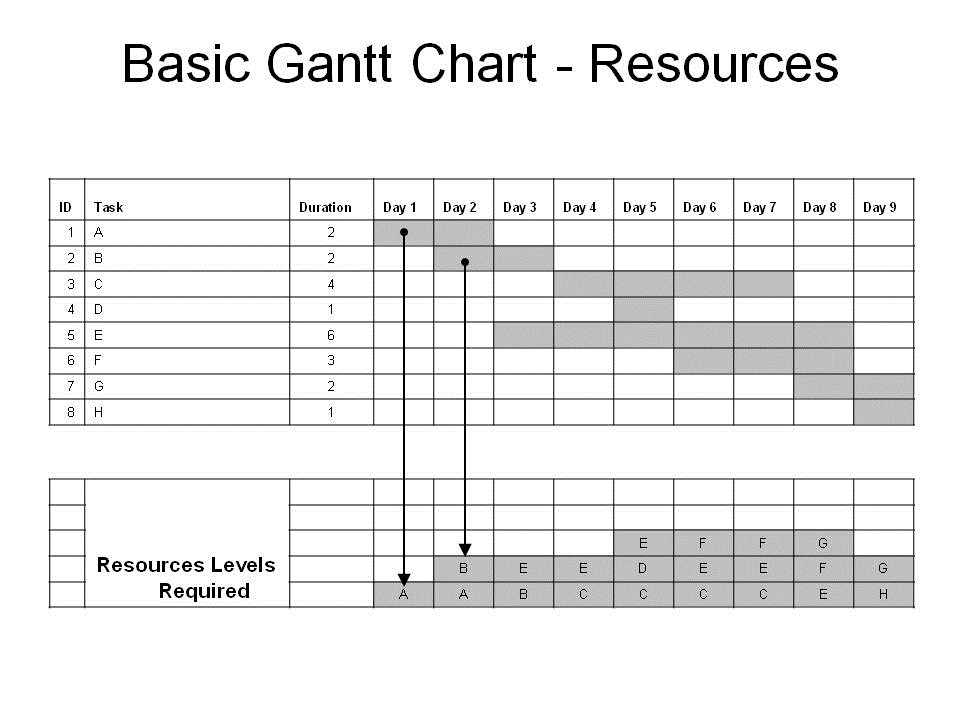
\includegraphics[width = 10.5cm]{oldnotes/Slide35.jpg}
\end{figure}
\end{frame}
\begin{center}\line(1,0){250}\end{center}





\begin{frame}
\begin{figure}
	\centering
		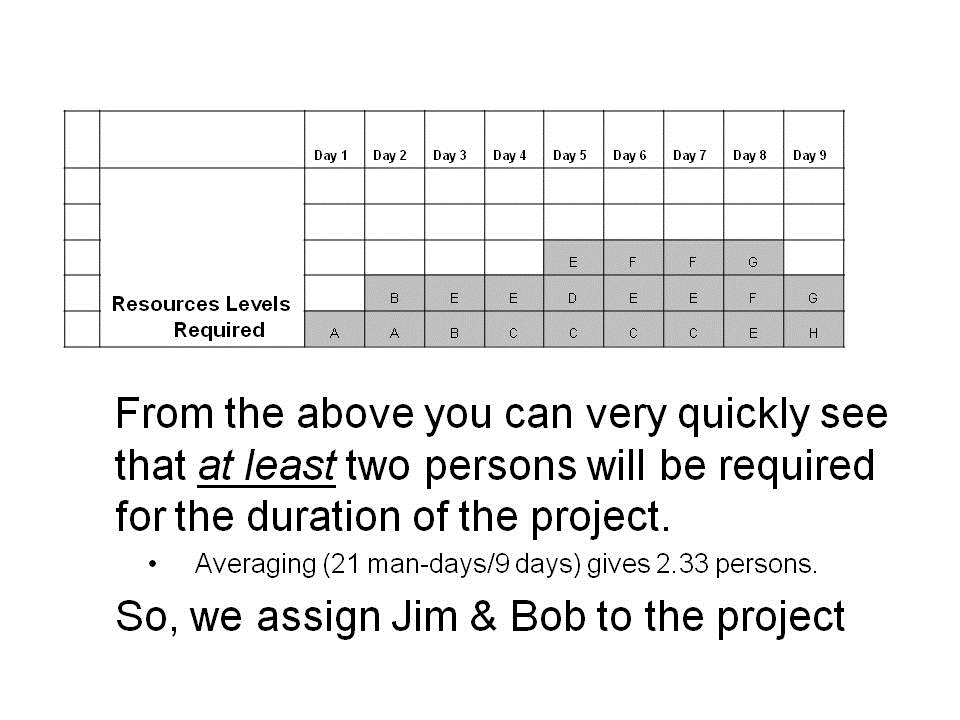
\includegraphics[width = 10.5cm]{oldnotes/Slide36.jpg}
\end{figure}
\end{frame}
\begin{center}\line(1,0){250}\end{center}





\begin{frame}
\begin{figure}
	\centering
		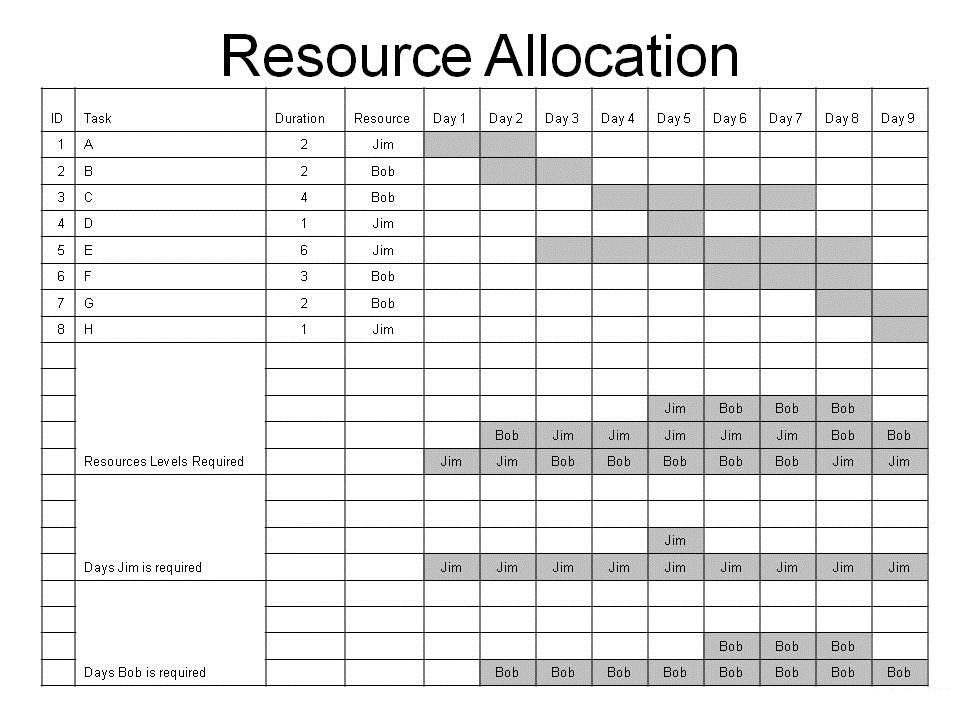
\includegraphics[width = 10.5cm]{oldnotes/Slide37.jpg}
\end{figure}
\end{frame}
\begin{center}\line(1,0){250}\end{center}





\begin{frame}
\begin{figure}
	\centering
		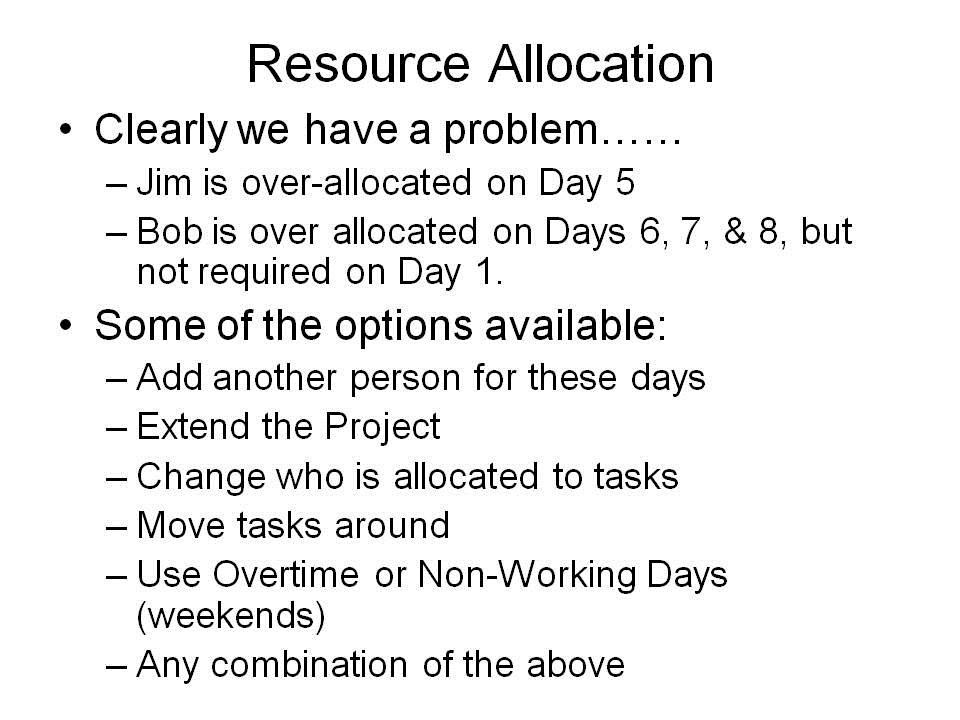
\includegraphics[width = 10.5cm]{oldnotes/Slide38.jpg}
\end{figure}
\end{frame}
\begin{center}\line(1,0){250}\end{center}





\begin{frame}
\begin{figure}
	\centering
		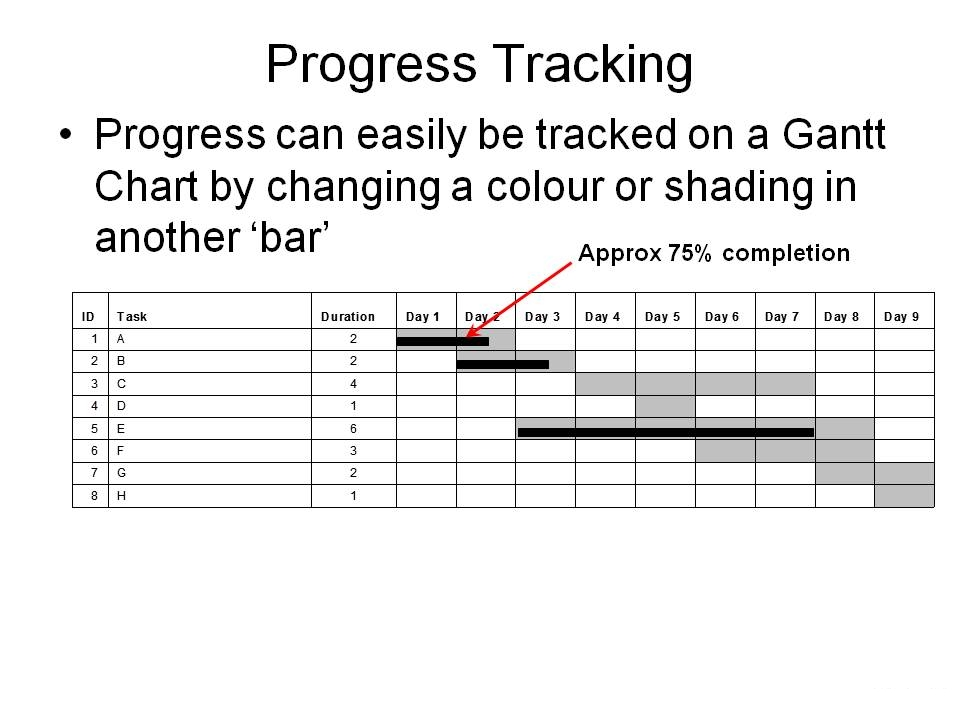
\includegraphics[width = 10.5cm]{oldnotes/Slide39.jpg}
\end{figure}
\end{frame}
\begin{center}\line(1,0){250}\end{center}





\begin{frame}
\begin{figure}
	\centering
		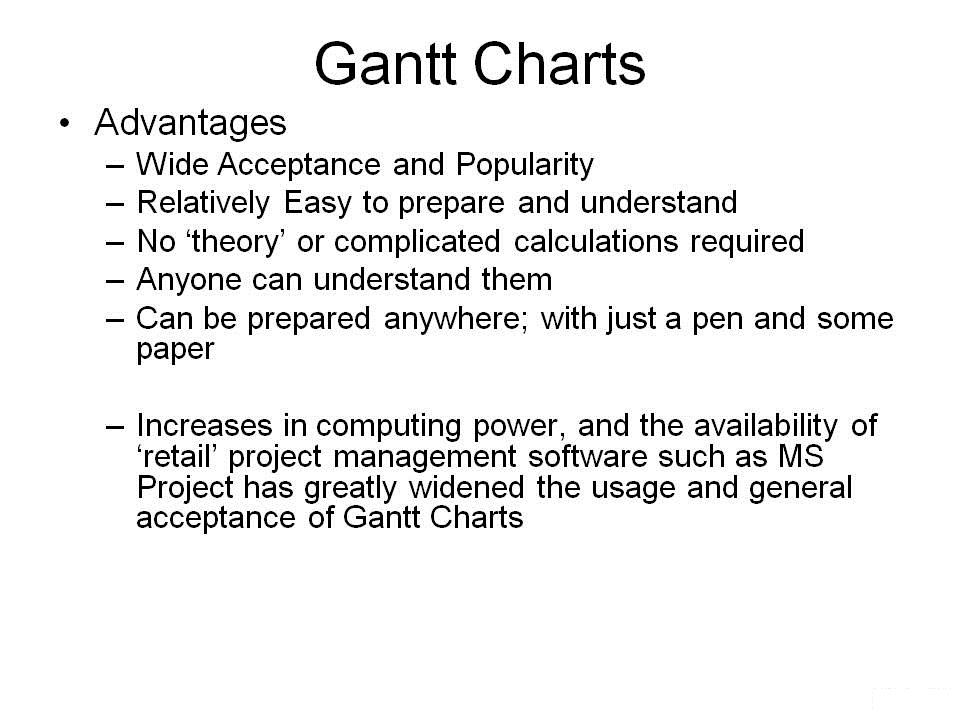
\includegraphics[width = 10.5cm]{oldnotes/Slide40.jpg}
\end{figure}
\end{frame}
\begin{center}\line(1,0){250}\end{center}





\begin{frame}
\begin{figure}
	\centering
		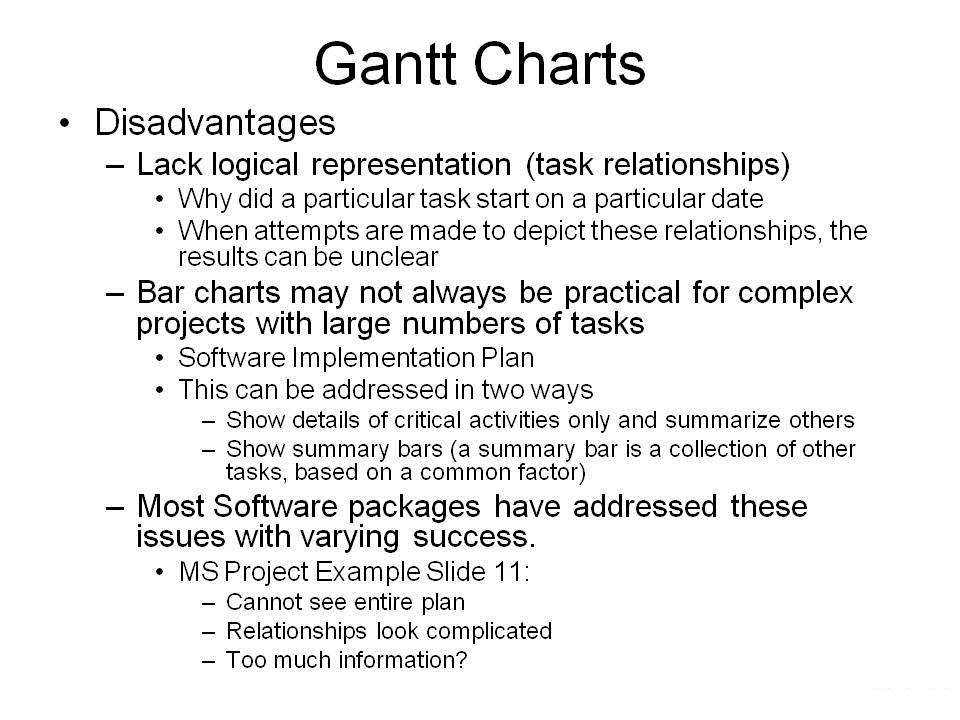
\includegraphics[width = 10.5cm]{oldnotes/Slide41.jpg}
\end{figure}
\end{frame}
\begin{center}\line(1,0){250}\end{center}





\begin{frame}
\begin{figure}
	\centering
		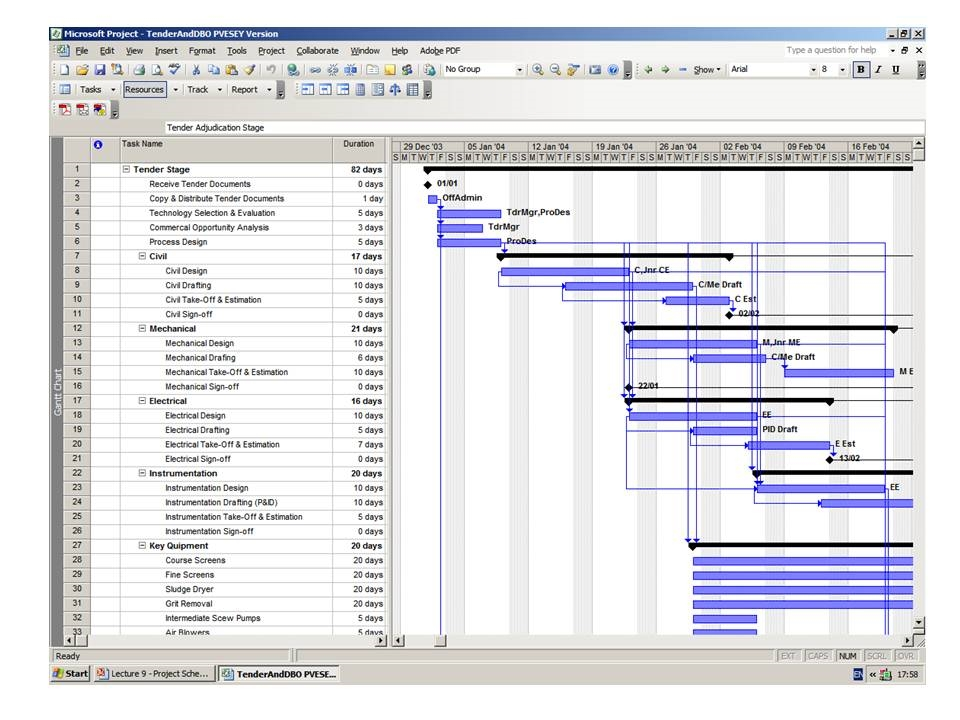
\includegraphics[width = 10.5cm]{oldnotes/Slide42.jpg}
\end{figure}
\end{frame}
\begin{center}\line(1,0){250}\end{center}





\begin{frame}
\begin{figure}
	\centering
		
\includegraphics[width = 10.5cm]{oldnotes/Slide43.jpg}
\end{figure}
\end{frame}
\begin{center}\line(1,0){250}\end{center}





\begin{frame}
\begin{figure}
	\centering
		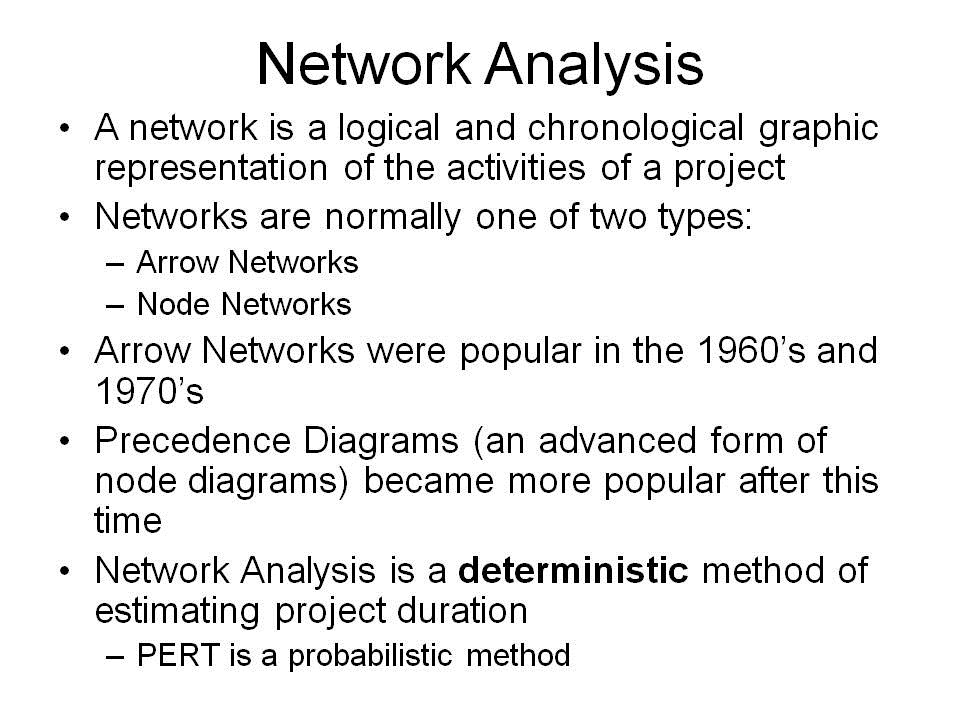
\includegraphics[width = 10.5cm]{oldnotes/Slide44.jpg}
\end{figure}
\end{frame}
\begin{center}\line(1,0){250}\end{center}





\begin{frame}
\begin{figure}
	\centering
		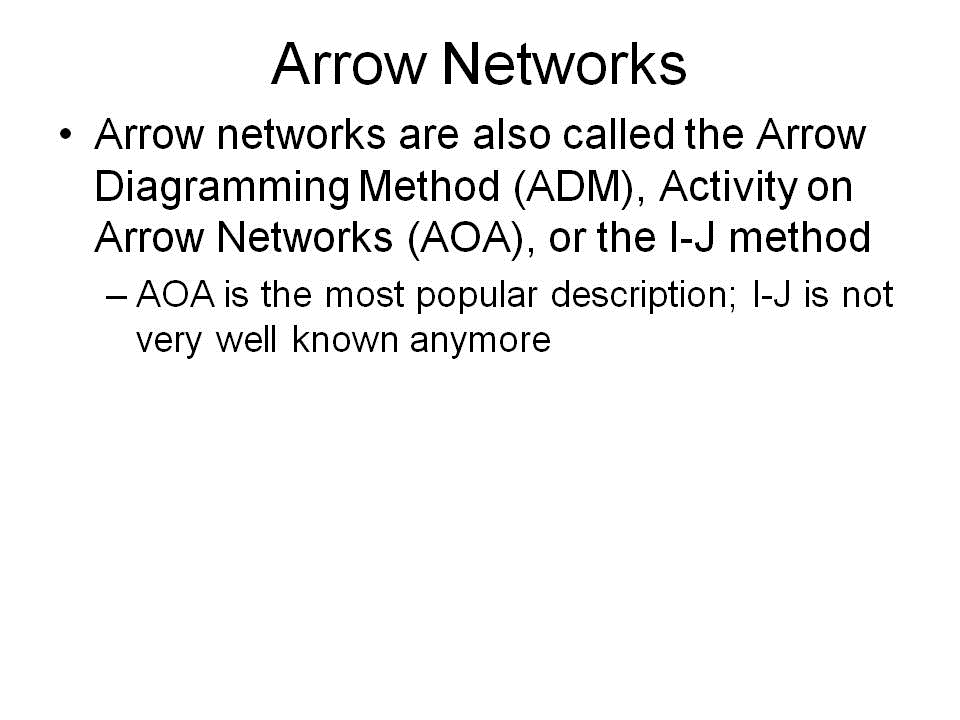
\includegraphics[width = 10.5cm]{oldnotes/Slide45.jpg}
\end{figure}
\end{frame}
\begin{center}\line(1,0){250}\end{center}





\begin{frame}
\begin{figure}
	\centering
		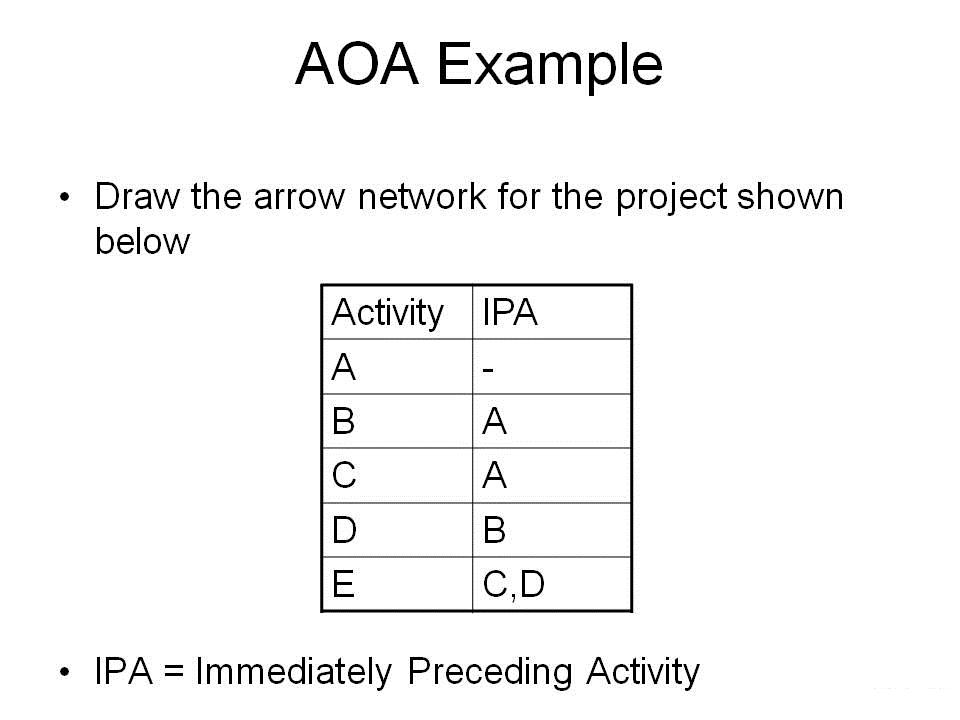
\includegraphics[width = 10.5cm]{oldnotes/Slide46.jpg}
\end{figure}
\end{frame}
\begin{center}\line(1,0){250}\end{center}





\begin{frame}
\begin{figure}
	\centering
		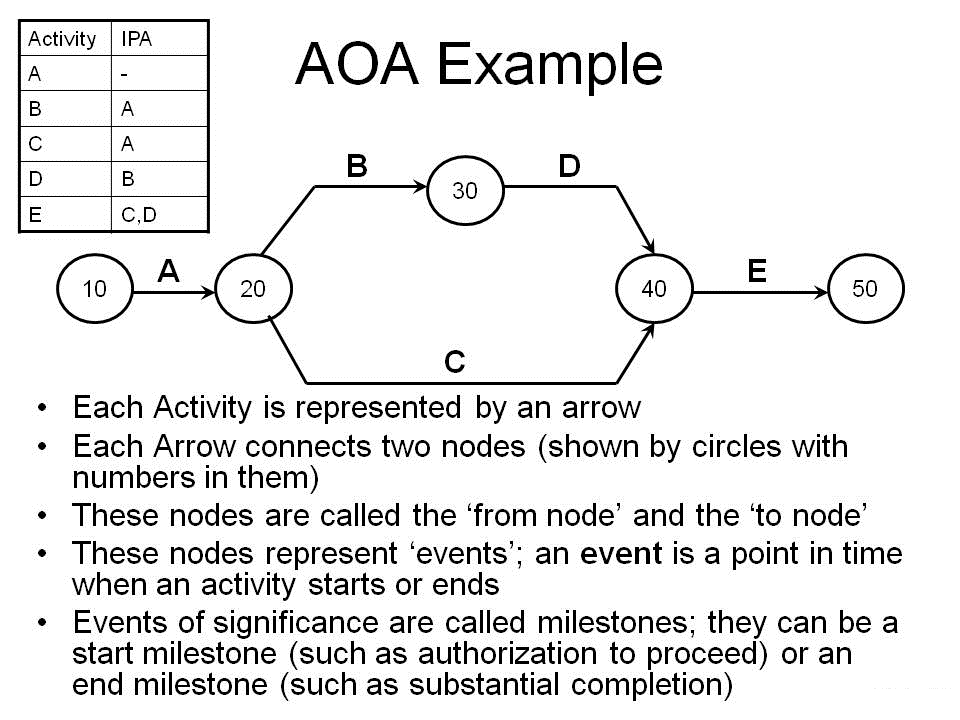
\includegraphics[width = 10.5cm]{oldnotes/Slide47.jpg}
\end{figure}
\end{frame}
\begin{center}\line(1,0){250}\end{center}





\begin{frame}
\begin{figure}
	\centering
		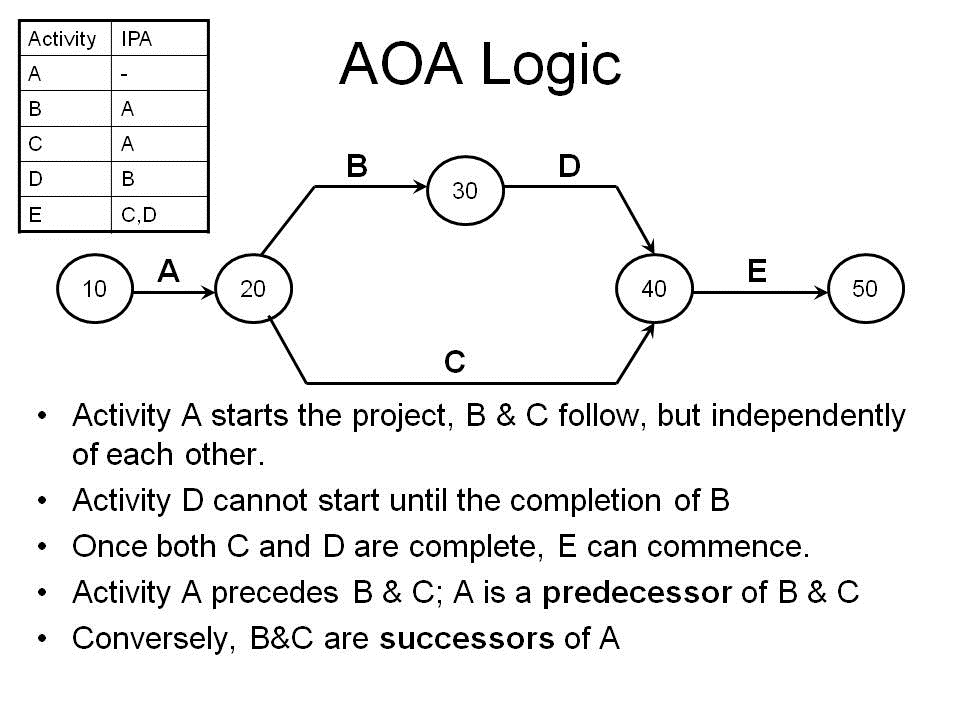
\includegraphics[width = 10.5cm]{oldnotes/Slide48.jpg}
\end{figure}
\end{frame}
\begin{center}\line(1,0){250}\end{center}





\begin{frame}
\begin{figure}
	\centering
		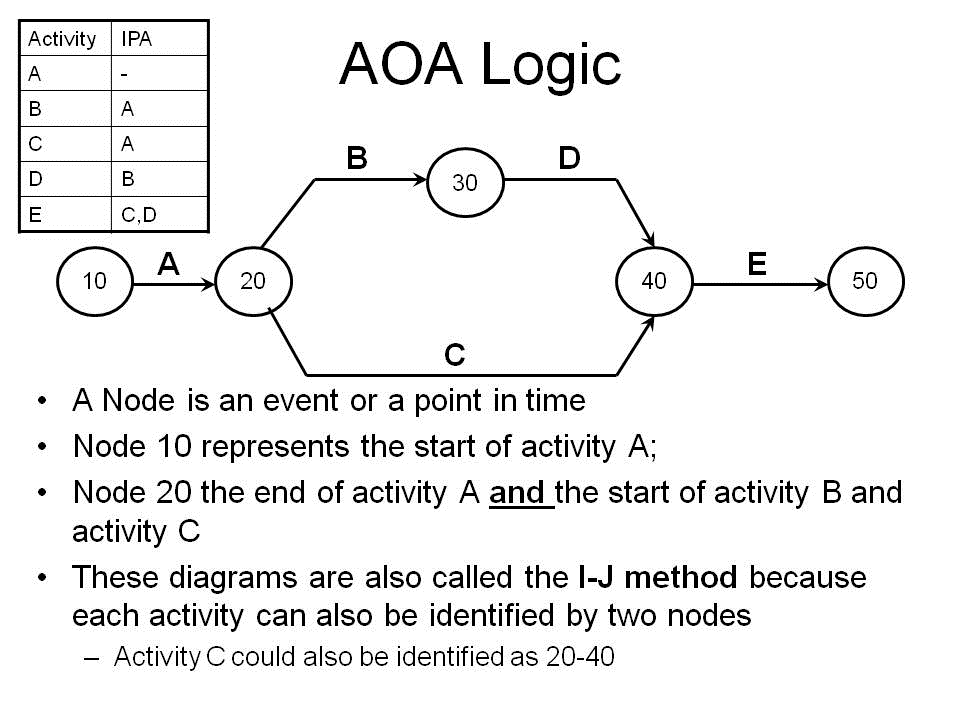
\includegraphics[width = 10.5cm]{oldnotes/Slide49.jpg}
\end{figure}
\end{frame}
\begin{center}\line(1,0){250}\end{center}





\begin{frame}
\begin{figure}
	\centering
		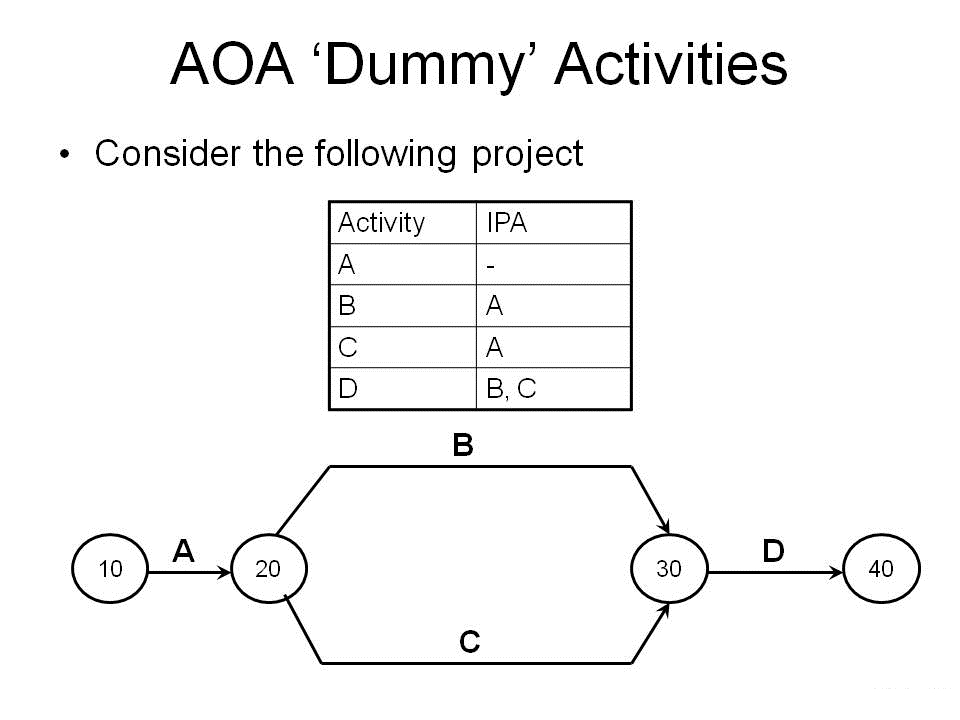
\includegraphics[width = 10.5cm]{oldnotes/Slide50.jpg}
\end{figure}
\end{frame}
\begin{center}\line(1,0){250}\end{center}





\begin{frame}
\begin{figure}
	\centering
		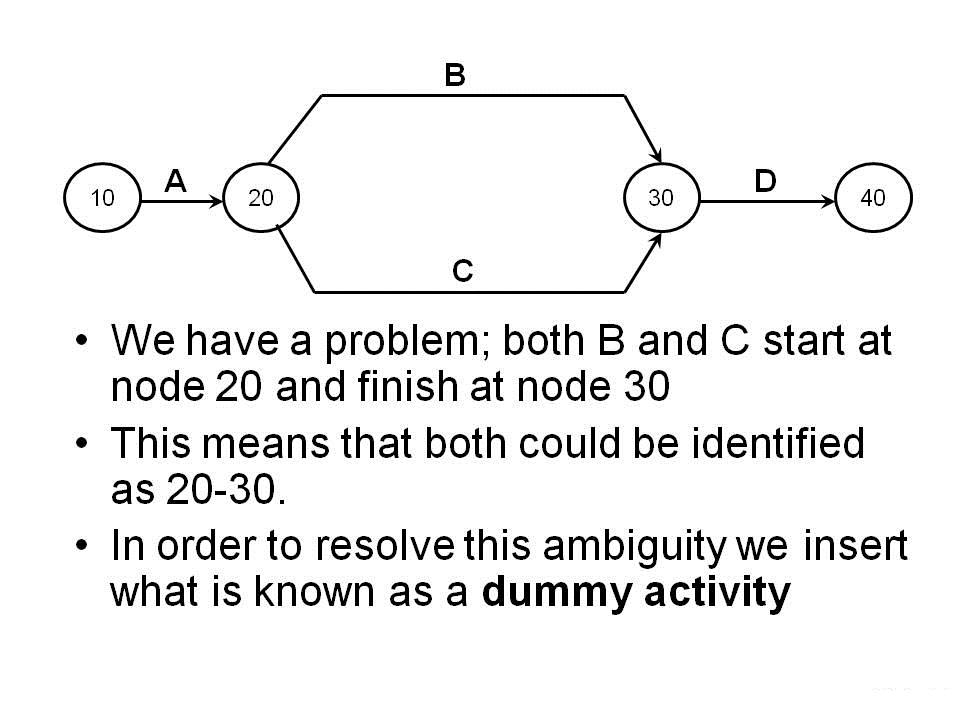
\includegraphics[width = 10.5cm]{oldnotes/Slide51.jpg}
\end{figure}
\end{frame}
\begin{center}\line(1,0){250}\end{center}





\begin{frame}
\begin{figure}
	\centering
		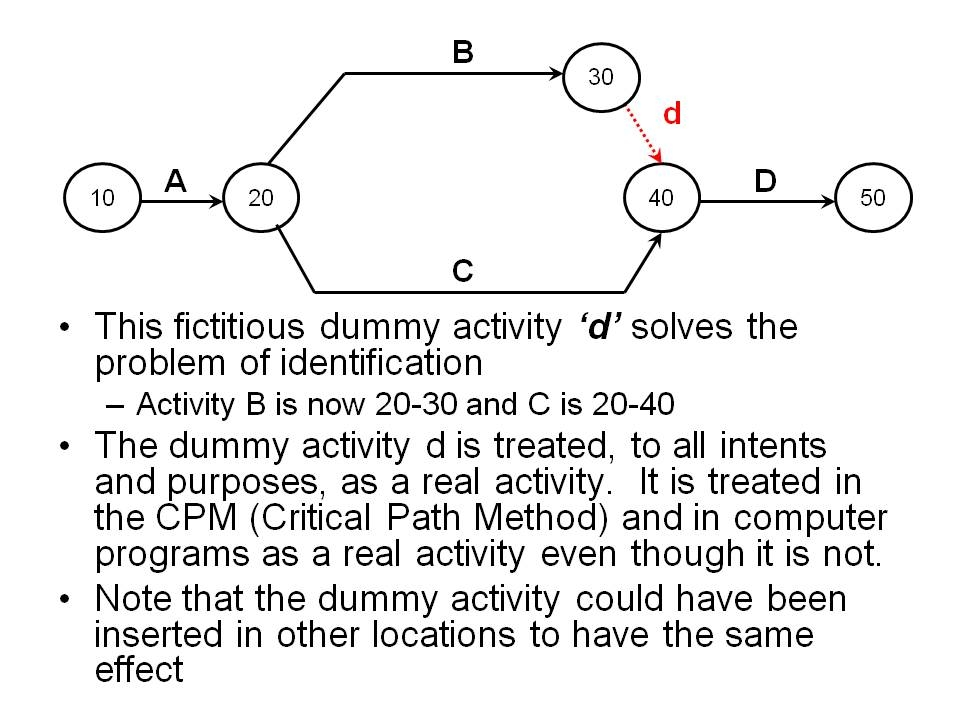
\includegraphics[width = 10.5cm]{oldnotes/Slide52.jpg}
\end{figure}
\end{frame}
\begin{center}\line(1,0){250}\end{center}





\begin{frame}
\begin{figure}
	\centering
		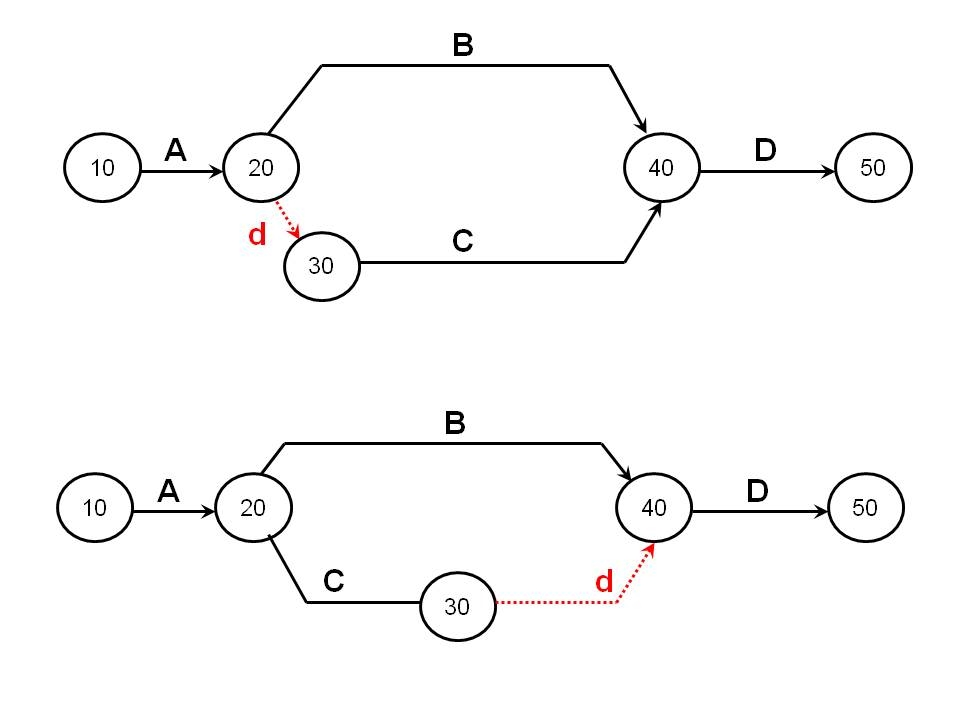
\includegraphics[width = 10.5cm]{oldnotes/Slide53.jpg}
\end{figure}
\end{frame}
\begin{center}\line(1,0){250}\end{center}





\begin{frame}
\begin{figure}
	\centering
		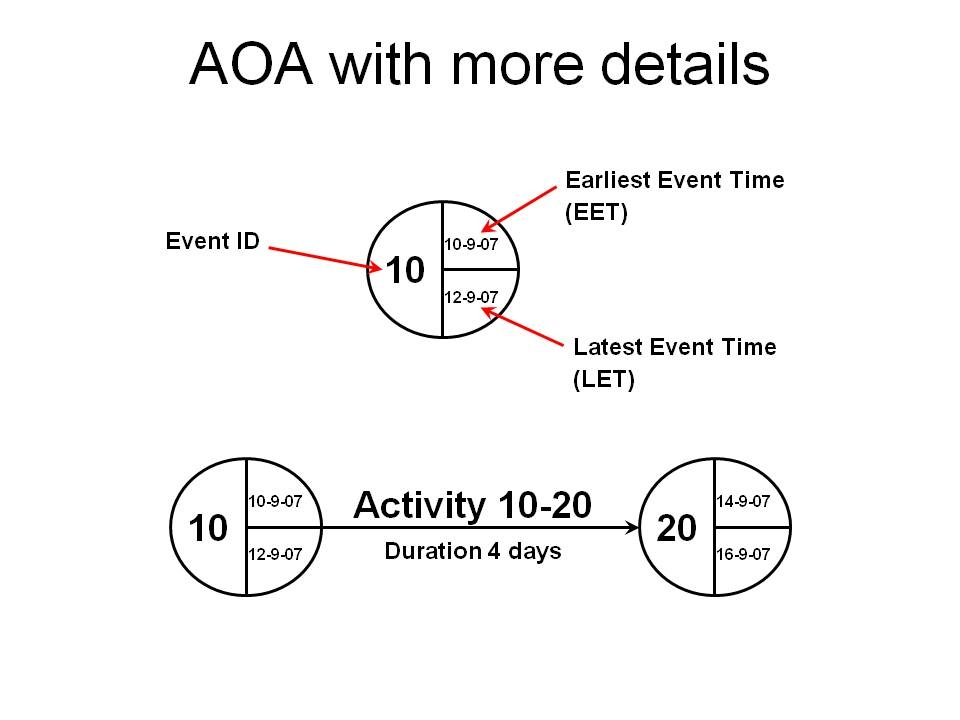
\includegraphics[width = 10.5cm]{oldnotes/Slide54.jpg}
\end{figure}
\end{frame}
\begin{center}\line(1,0){250}\end{center}





\begin{frame}
\begin{figure}
	\centering
		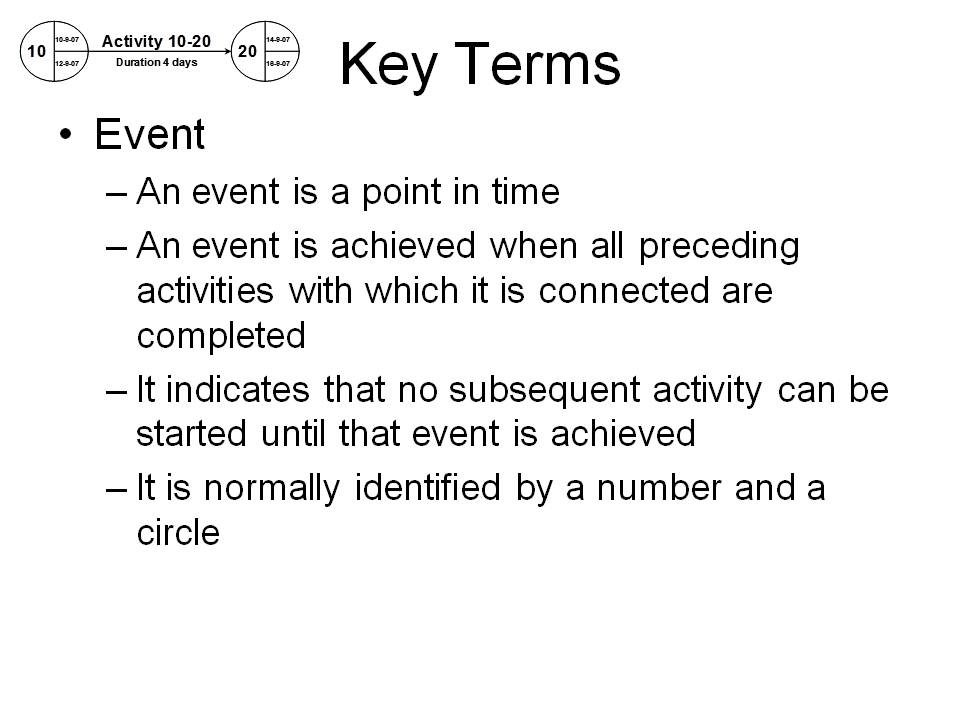
\includegraphics[width = 10.5cm]{oldnotes/Slide55.jpg}
\end{figure}
\end{frame}
\begin{center}\line(1,0){250}\end{center}





\begin{frame}
\begin{figure}
	\centering
		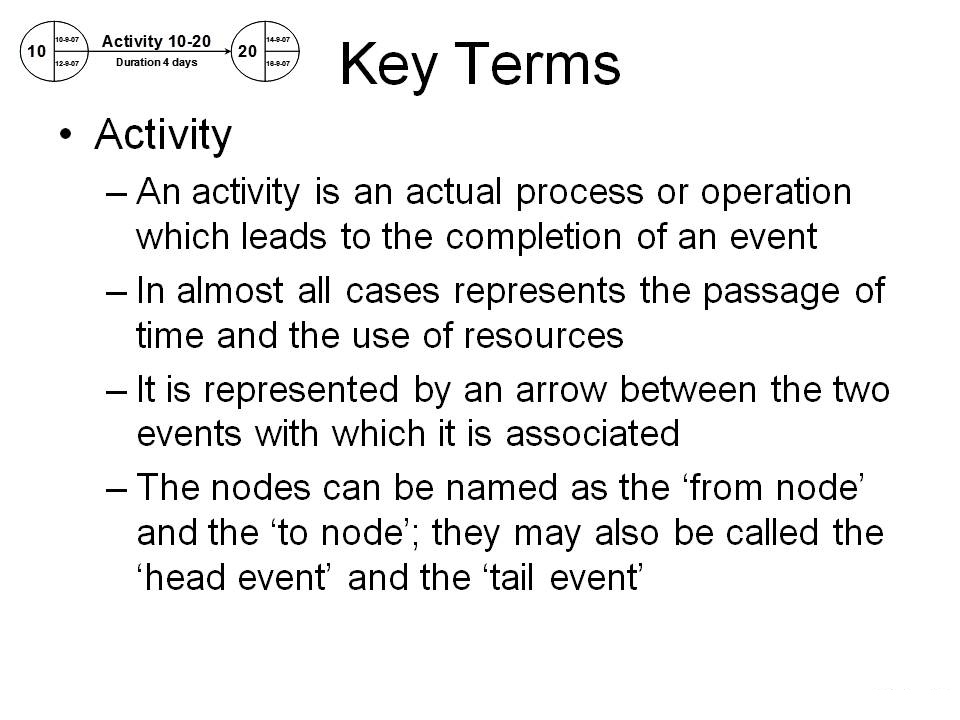
\includegraphics[width = 10.5cm]{oldnotes/Slide56.jpg}
\end{figure}
\end{frame}
\begin{center}\line(1,0){250}\end{center}





\begin{frame}
\begin{figure}
	\centering
		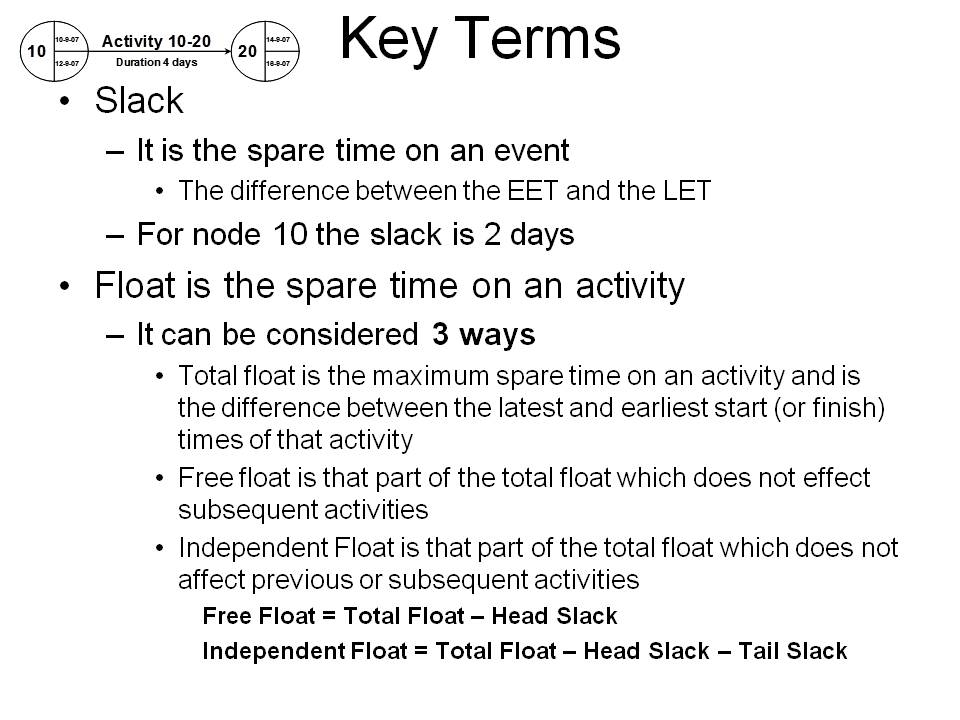
\includegraphics[width = 10.5cm]{oldnotes/Slide57.jpg}
\end{figure}
\end{frame}
\begin{center}\line(1,0){250}\end{center}





\begin{frame}
\begin{figure}
	\centering
		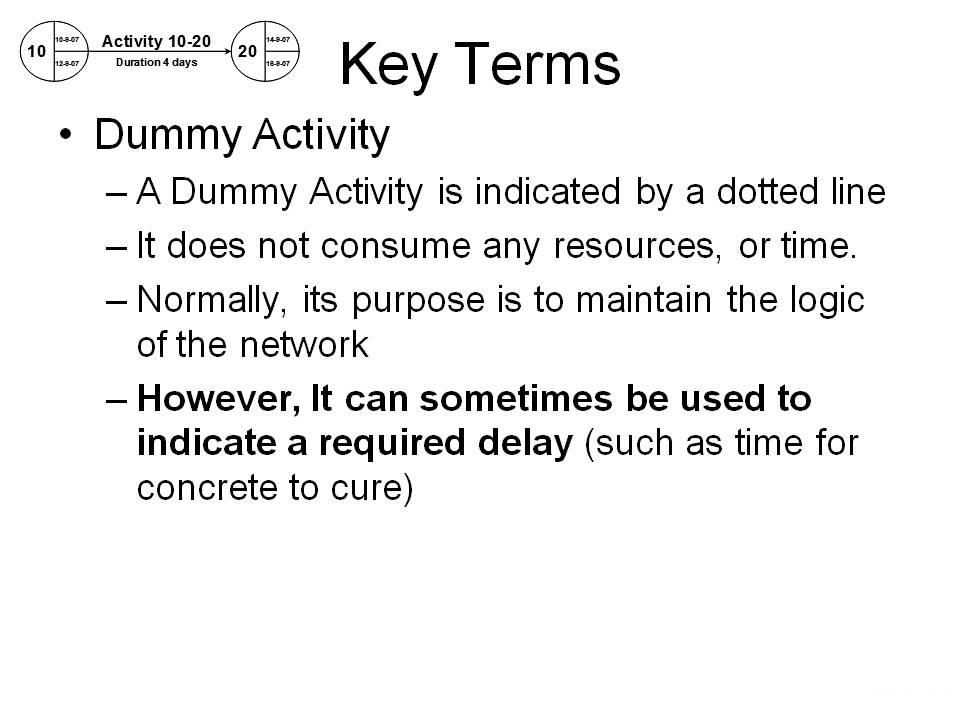
\includegraphics[width = 10.5cm]{oldnotes/Slide58.jpg}
\end{figure}
\end{frame}
\begin{center}\line(1,0){250}\end{center}









\section{Activity on Arrow}



\begin{frame}
\begin{figure}
	\centering
		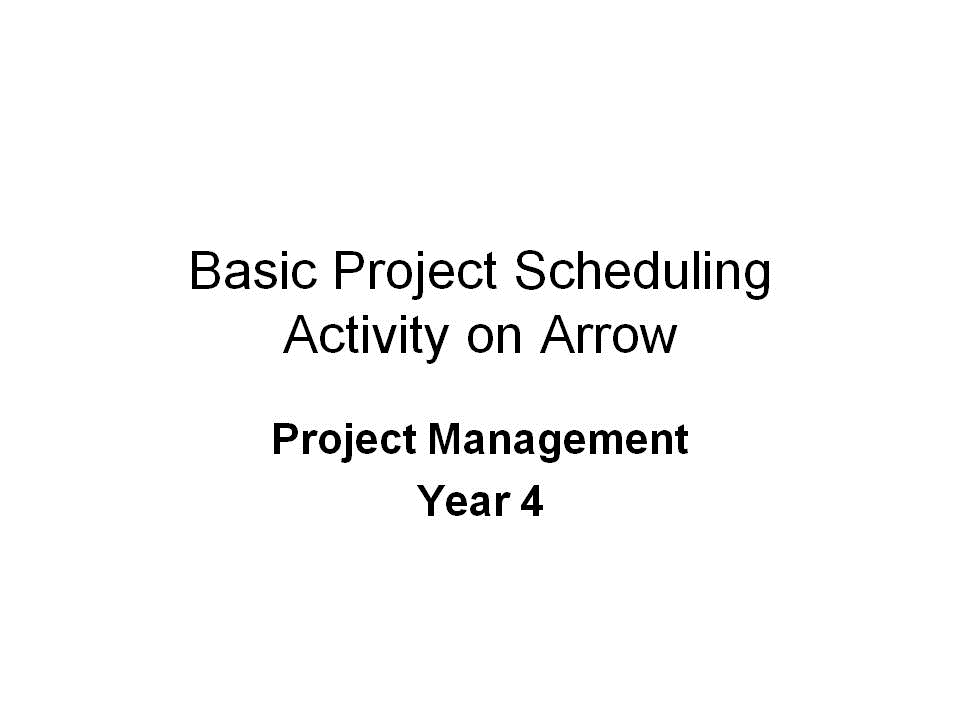
\includegraphics[width = 10.5cm]{oldnotes/Slide60.jpg}
\end{figure}
\end{frame}
\begin{center}\line(1,0){250}\end{center}


\begin{frame}
\begin{figure}
	\centering
		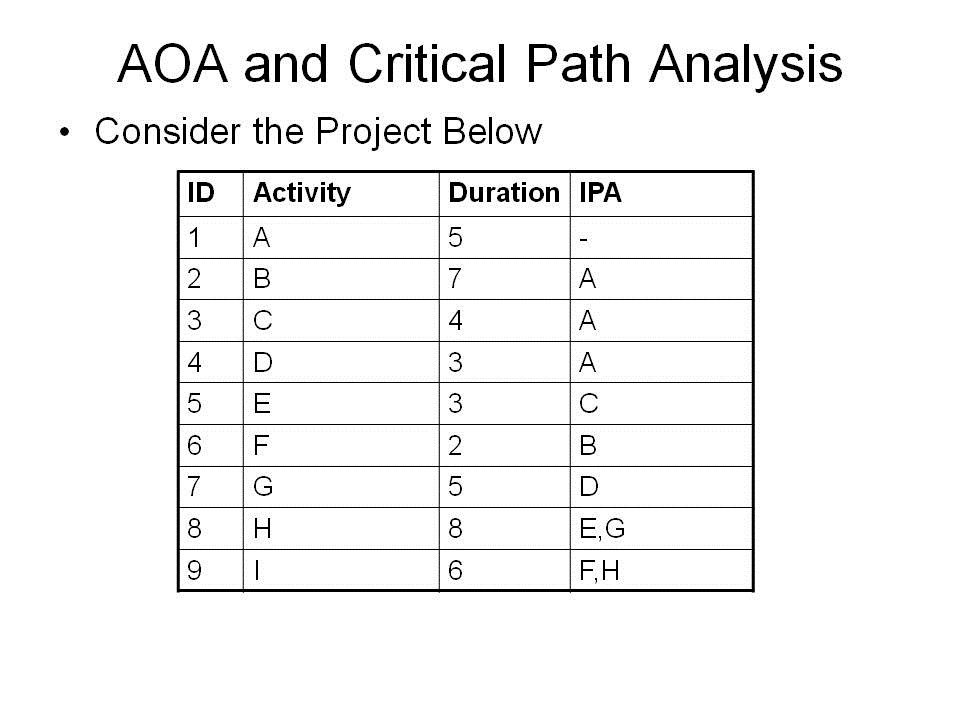
\includegraphics[width = 10.5cm]{oldnotes/Slide61.jpg}
\end{figure}
\end{frame}
\begin{center}\line(1,0){250}\end{center}



\begin{frame}
\begin{figure}
	\centering
		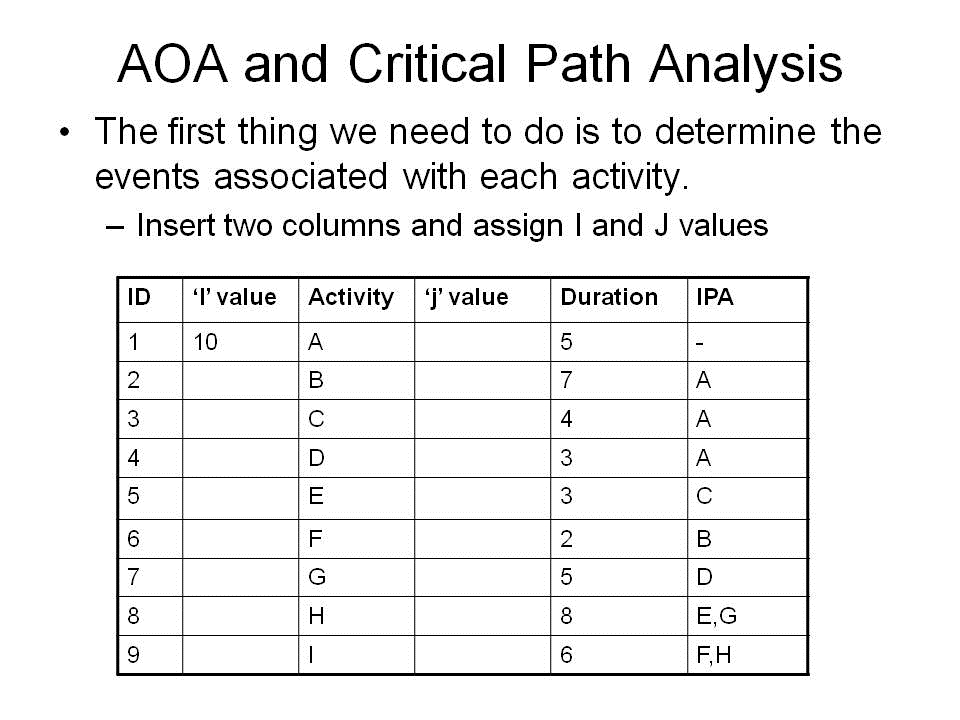
\includegraphics[width = 10.5cm]{oldnotes/Slide62.jpg}
\end{figure}
\end{frame}
\begin{center}\line(1,0){250}\end{center}


\begin{frame}
\begin{figure}
	\centering
		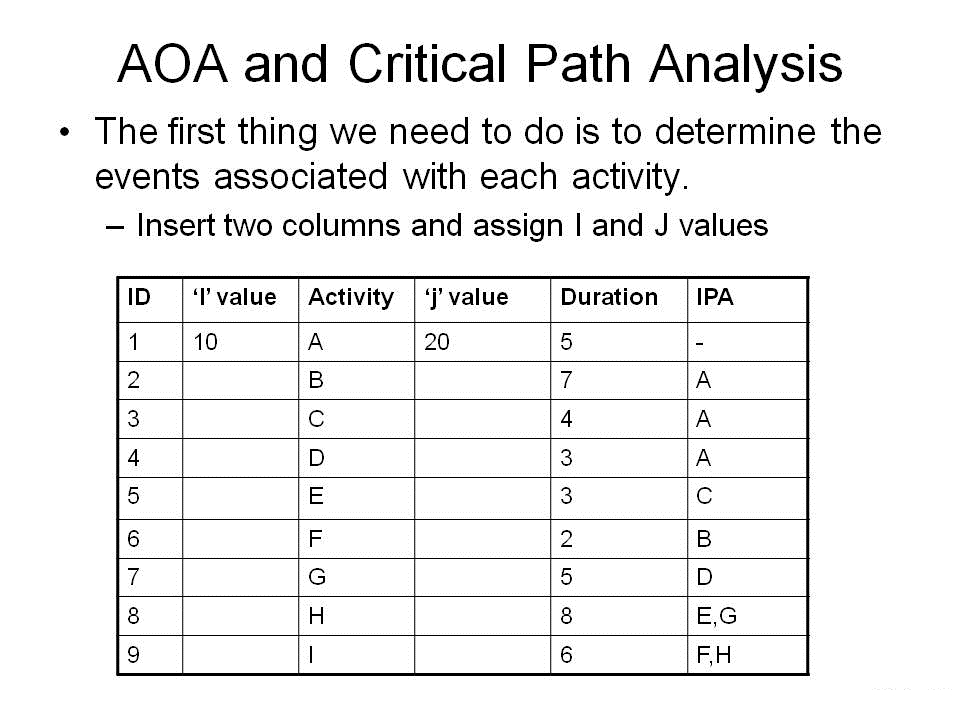
\includegraphics[width = 10.5cm]{oldnotes/Slide63.jpg}
\end{figure}
\end{frame}
\begin{center}\line(1,0){250}\end{center}


\begin{frame}
\begin{figure}
	\centering
		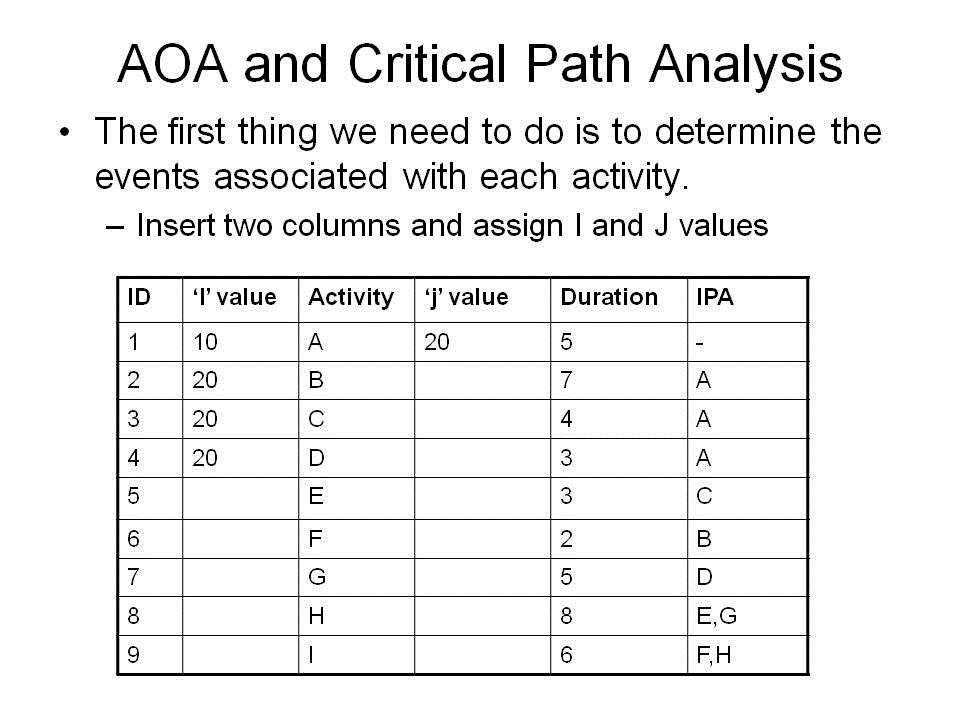
\includegraphics[width = 10.5cm]{oldnotes/Slide64.jpg}
\end{figure}
\end{frame}
\begin{center}\line(1,0){250}\end{center}


\begin{frame}
\begin{figure}
	\centering
		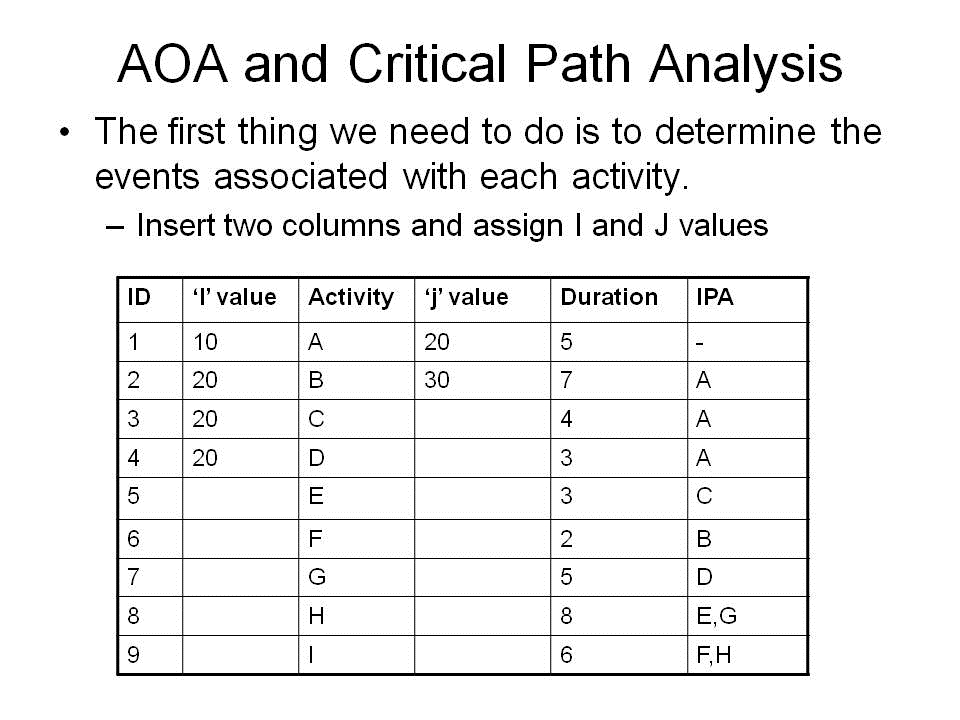
\includegraphics[width = 10.5cm]{oldnotes/Slide65.jpg}
\end{figure}
\end{frame}
\begin{center}\line(1,0){250}\end{center}


\begin{frame}
\begin{figure}
	\centering
		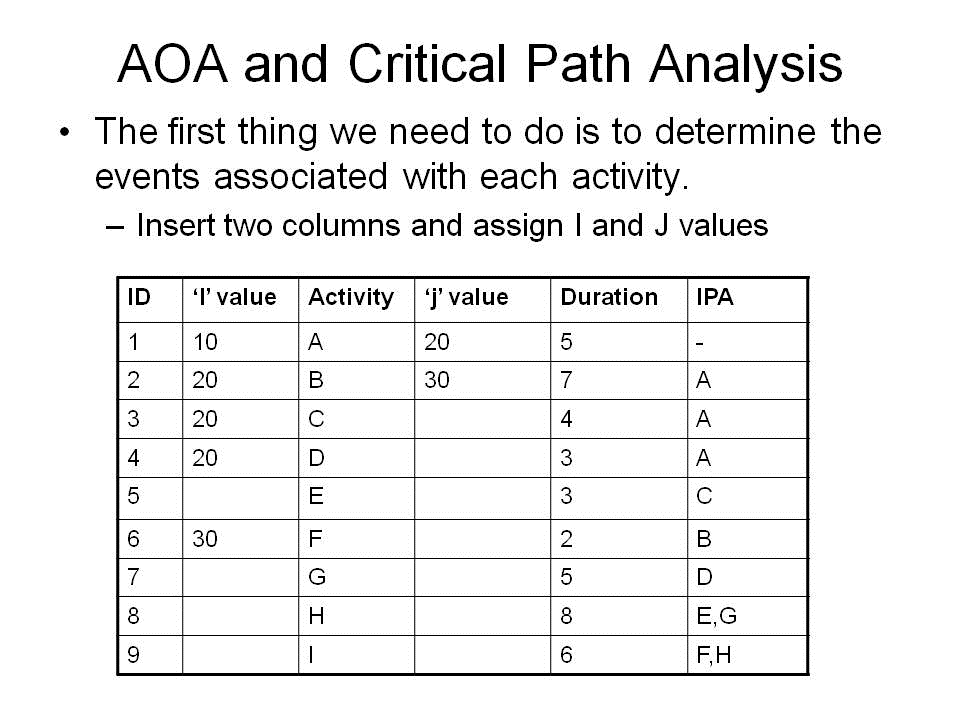
\includegraphics[width = 10.5cm]{oldnotes/Slide66.jpg}
\end{figure}
\end{frame}
\begin{center}\line(1,0){250}\end{center}


\begin{frame}
\begin{figure}
	\centering
		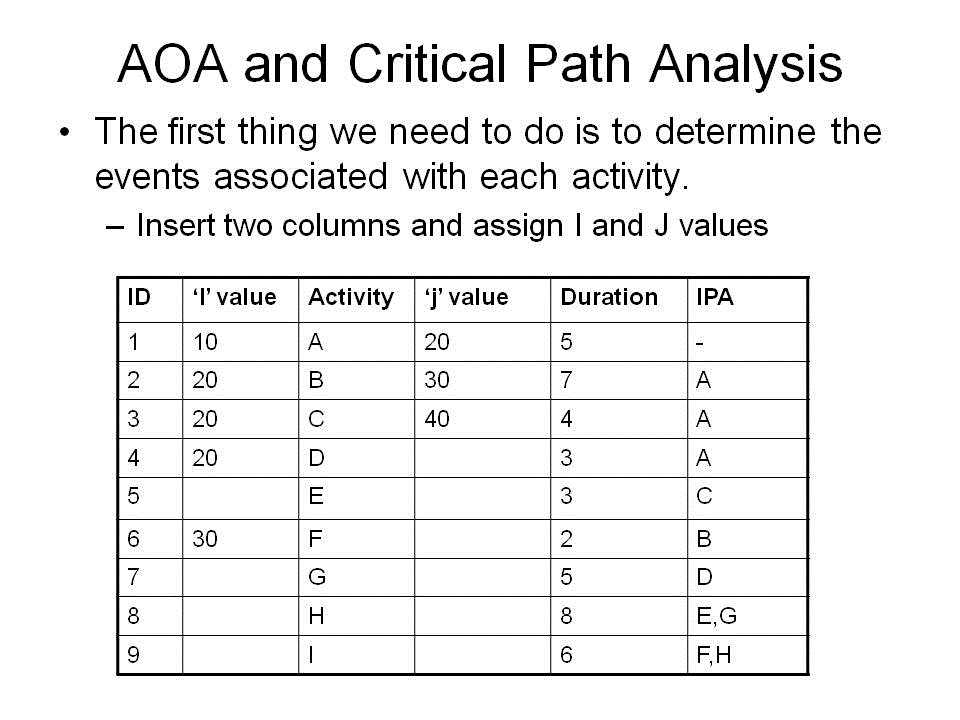
\includegraphics[width = 10.5cm]{oldnotes/Slide67.jpg}
\end{figure}
\end{frame}
\begin{center}\line(1,0){250}\end{center}


\begin{frame}
\begin{figure}
	\centering
		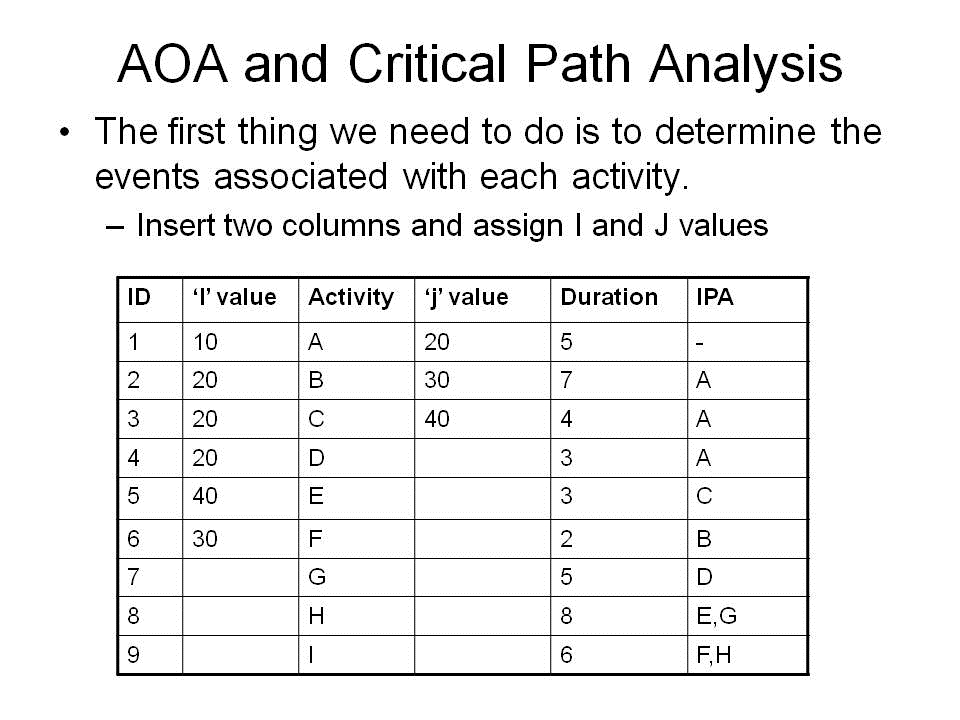
\includegraphics[width = 10.5cm]{oldnotes/Slide68.jpg}
\end{figure}
\end{frame}
\begin{center}\line(1,0){250}\end{center}


\begin{frame}
\begin{figure}
	\centering
		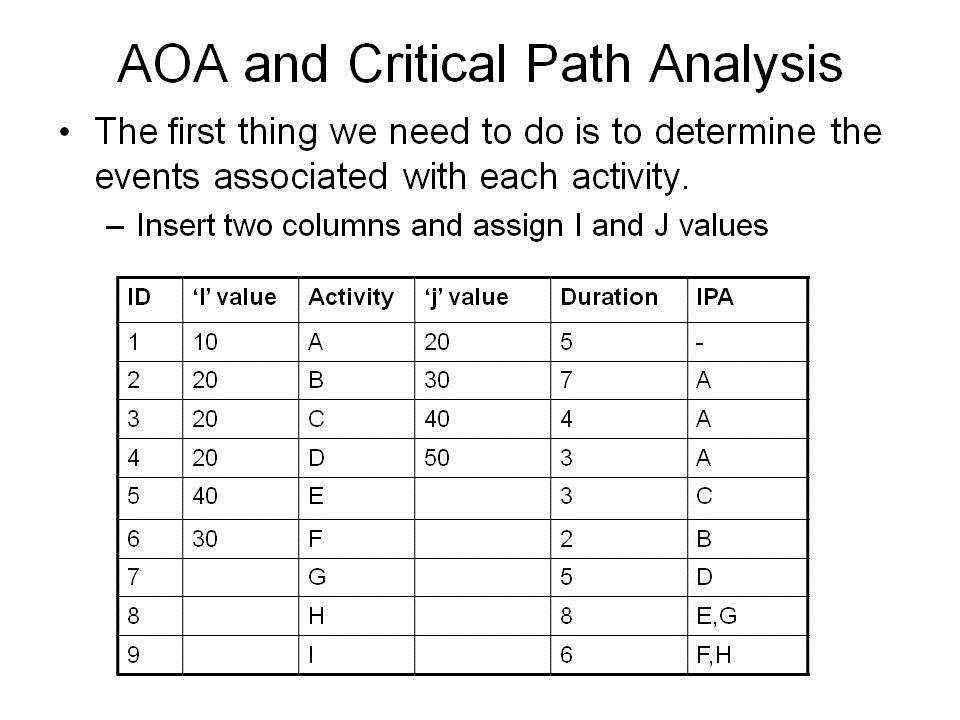
\includegraphics[width = 10.5cm]{oldnotes/Slide69.jpg}
\end{figure}
\end{frame}
\begin{center}\line(1,0){250}\end{center}


\begin{frame}
\begin{figure}
	\centering
		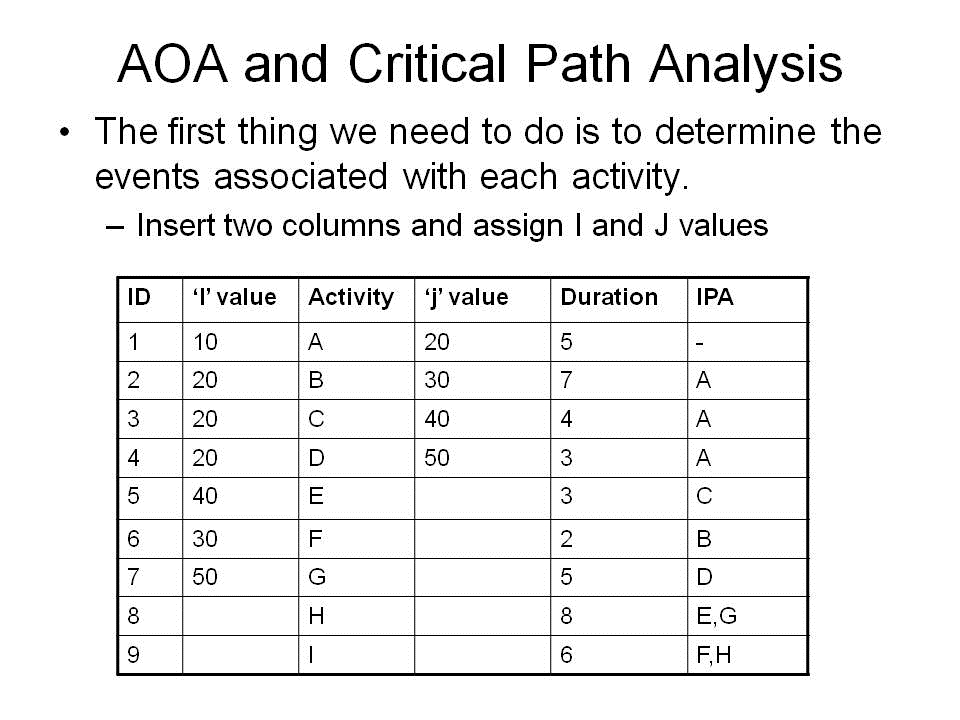
\includegraphics[width = 10.5cm]{oldnotes/Slide70.jpg}
\end{figure}
\end{frame}
\begin{center}\line(1,0){250}\end{center}


\begin{frame}
\begin{figure}
	\centering
		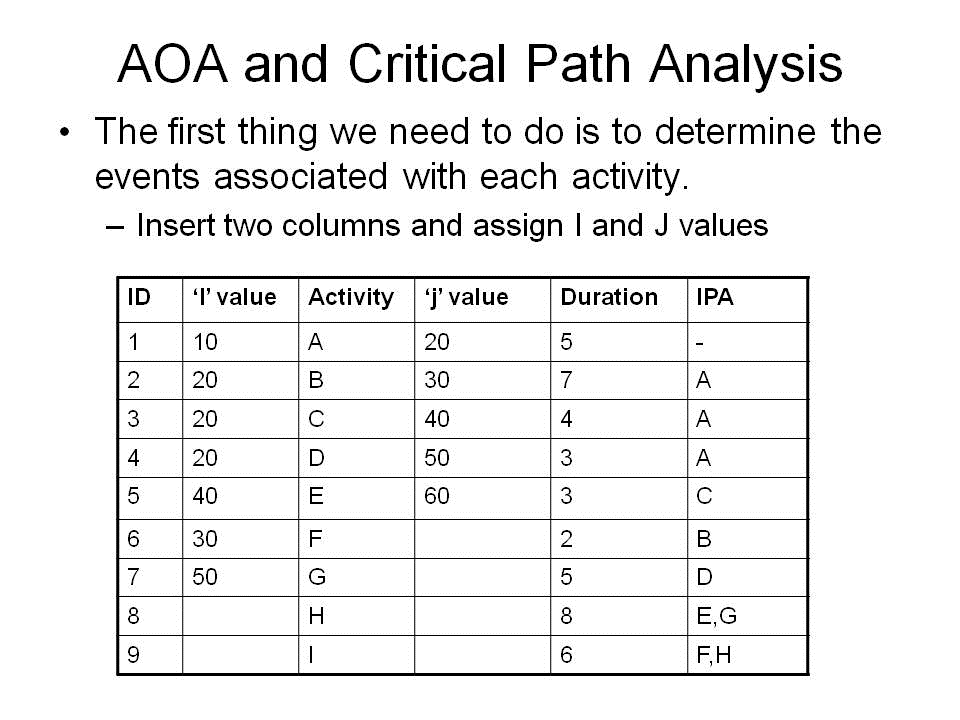
\includegraphics[width = 10.5cm]{oldnotes/Slide71.jpg}
\end{figure}
\end{frame}
\begin{center}\line(1,0){250}\end{center}


\begin{frame}
\begin{figure}
	\centering
		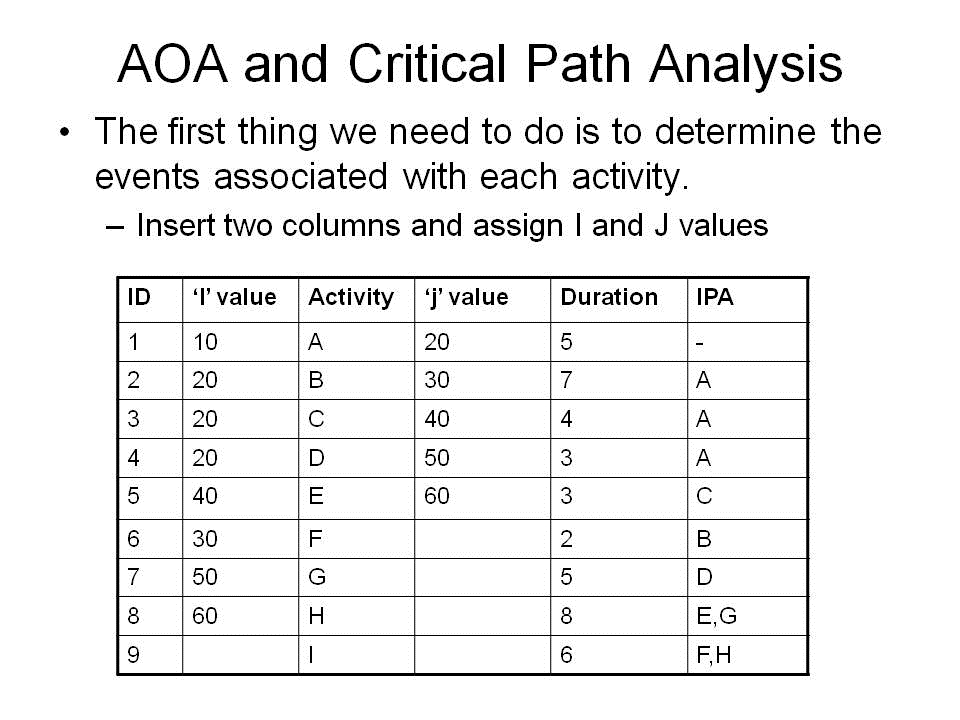
\includegraphics[width = 10.5cm]{oldnotes/Slide72.jpg}
\end{figure}
\end{frame}
\begin{center}\line(1,0){250}\end{center}


\begin{frame}
\begin{figure}
	\centering
		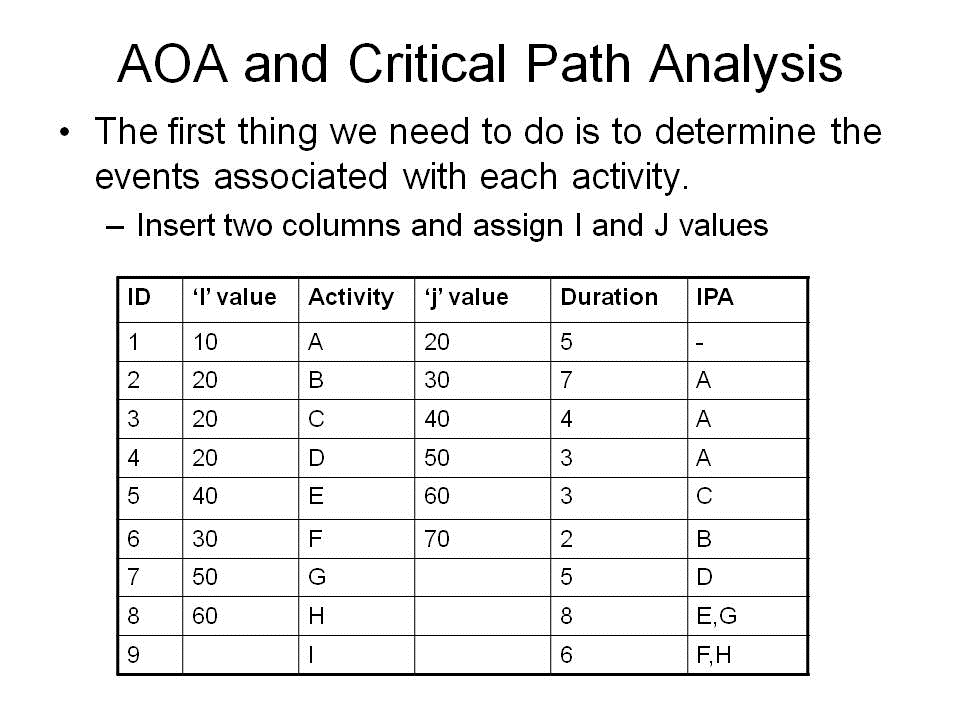
\includegraphics[width = 10.5cm]{oldnotes/Slide73.jpg}
\end{figure}
\end{frame}
\begin{center}\line(1,0){250}\end{center}


\begin{frame}
\begin{figure}
	\centering
		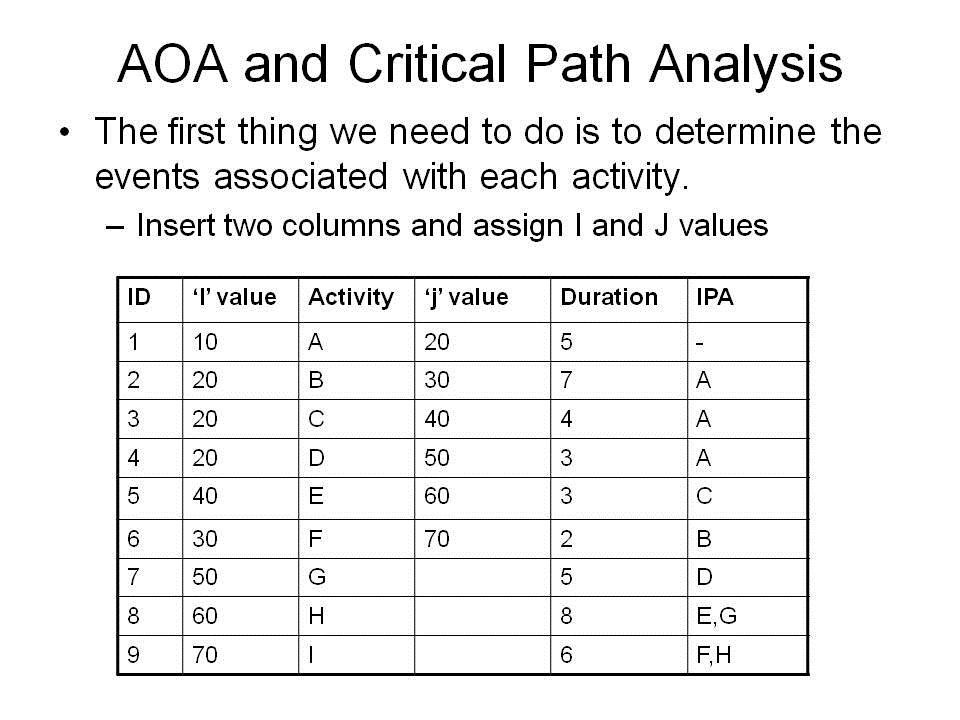
\includegraphics[width = 10.5cm]{oldnotes/Slide74.jpg}
\end{figure}
\end{frame}
\begin{center}\line(1,0){250}\end{center}


\begin{frame}
\begin{figure}
	\centering
		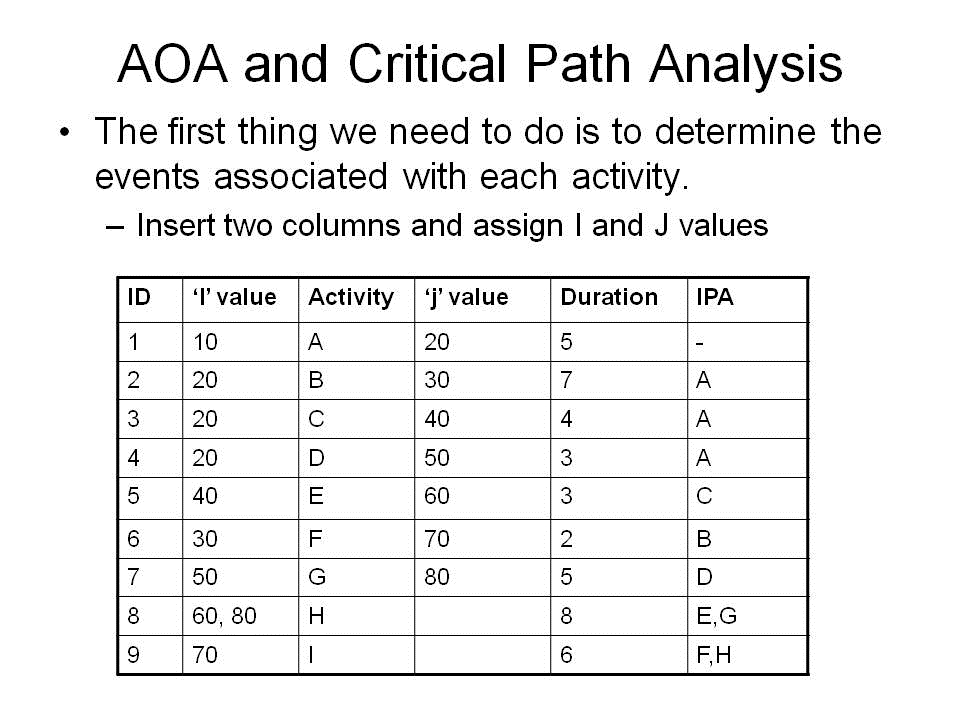
\includegraphics[width = 10.5cm]{oldnotes/Slide75.jpg}
\end{figure}
\end{frame}
\begin{center}\line(1,0){250}\end{center}


\begin{frame}
\begin{figure}
	\centering
		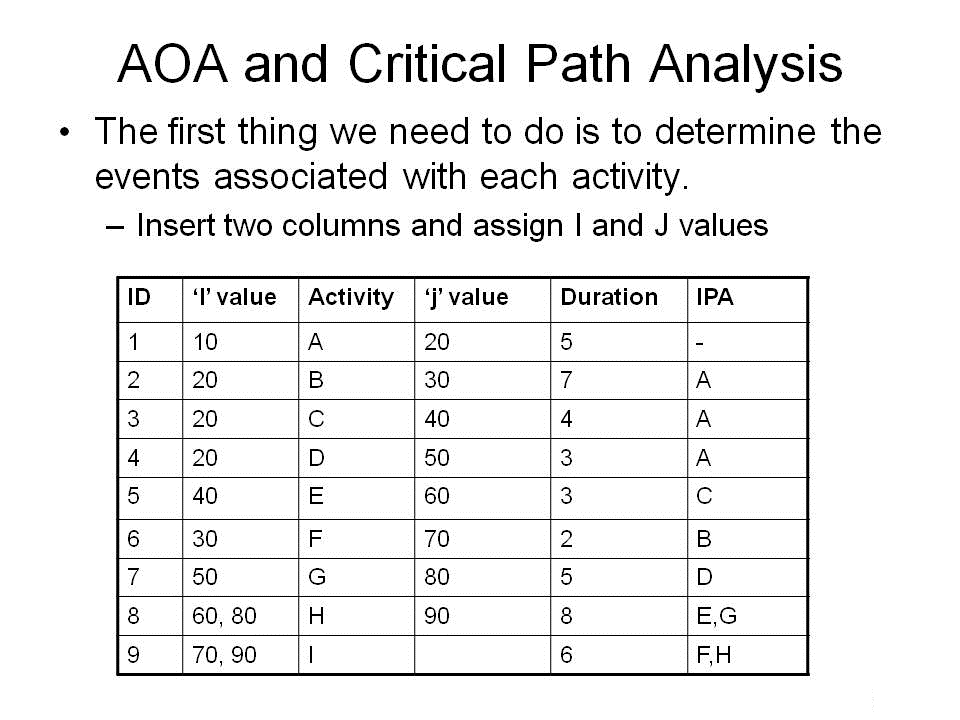
\includegraphics[width = 10.5cm]{oldnotes/Slide76.jpg}
\end{figure}
\end{frame}
\begin{center}\line(1,0){250}\end{center}


\begin{frame}
\begin{figure}
	\centering
		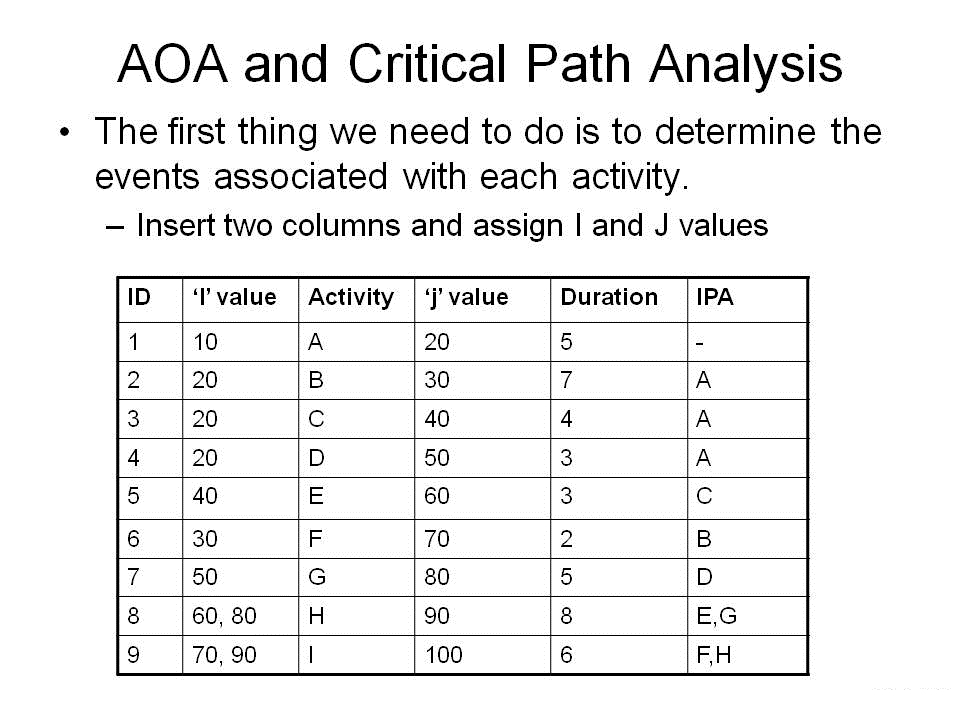
\includegraphics[width = 10.5cm]{oldnotes/Slide77.jpg}
\end{figure}
\end{frame}
\begin{center}\line(1,0){250}\end{center}


\begin{frame}
\begin{figure}
	\centering
		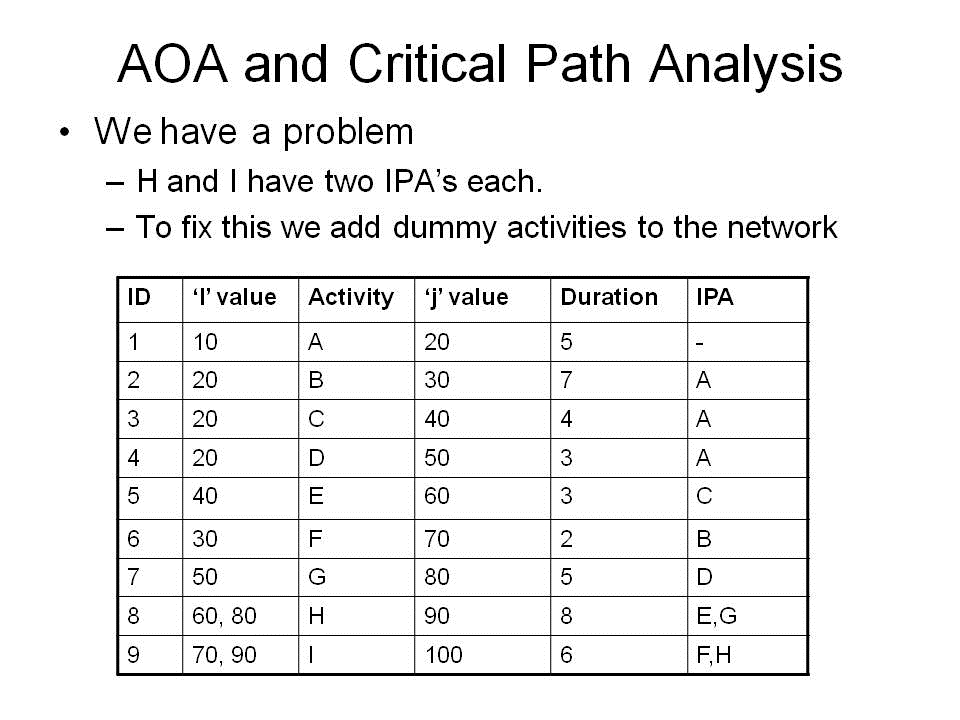
\includegraphics[width = 10.5cm]{oldnotes/Slide78.jpg}
\end{figure}
\end{frame}
\begin{center}\line(1,0){250}\end{center}


\begin{frame}
\begin{figure}
	\centering
		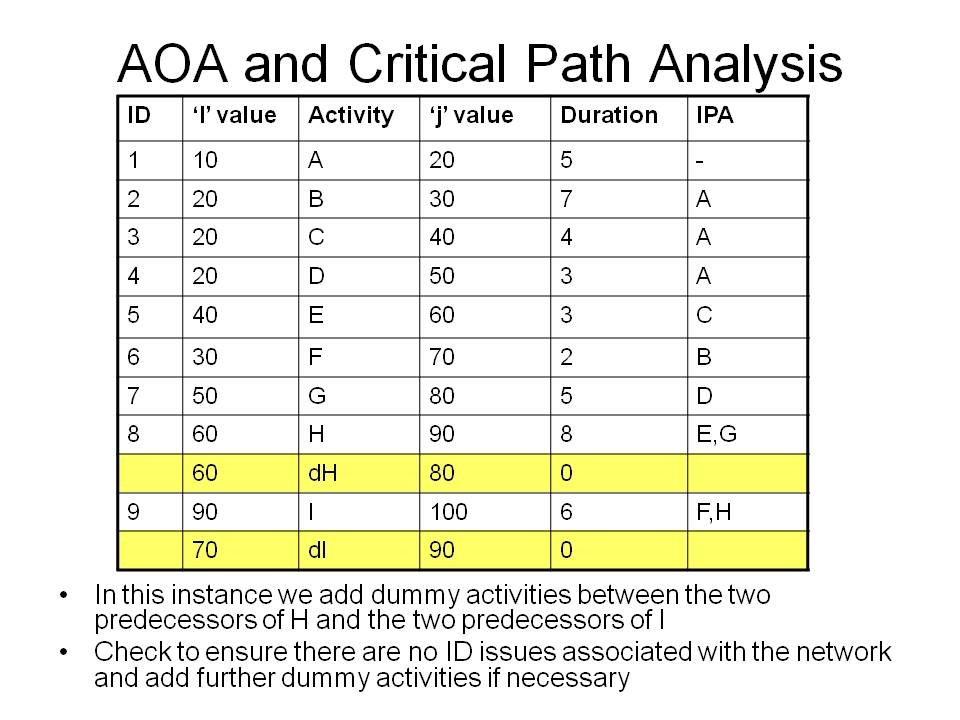
\includegraphics[width = 10.5cm]{oldnotes/Slide79.jpg}
\end{figure}
\end{frame}
\begin{center}\line(1,0){250}\end{center}


\begin{frame}
\begin{figure}
	\centering
		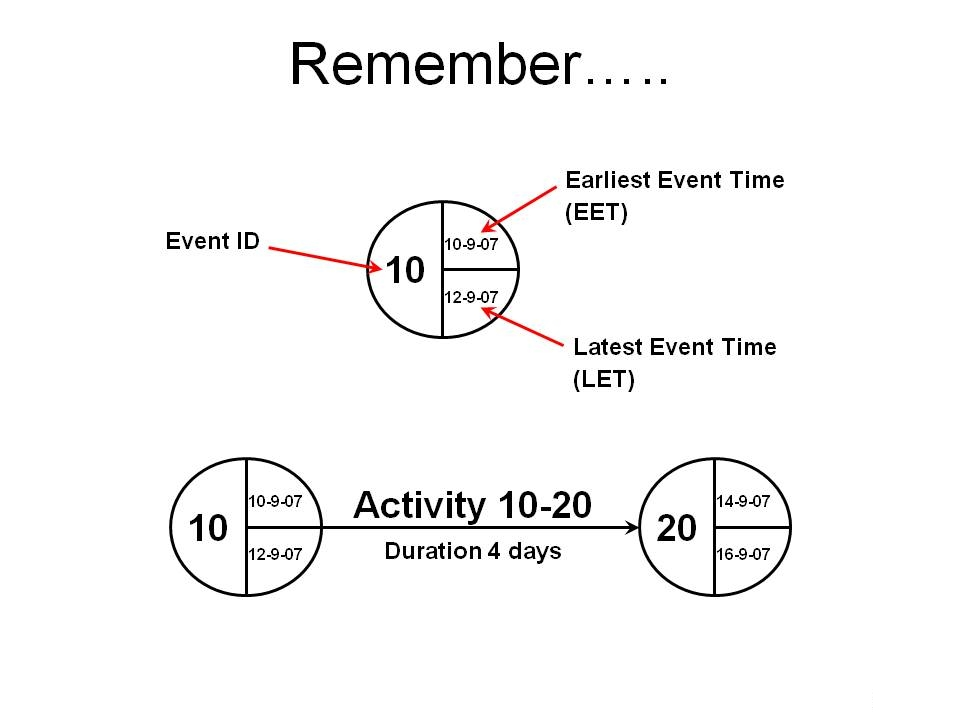
\includegraphics[width = 10.5cm]{oldnotes/Slide80.jpg}
\end{figure}
\end{frame}
\begin{center}\line(1,0){250}\end{center}


\begin{frame}
\begin{figure}
	\centering
		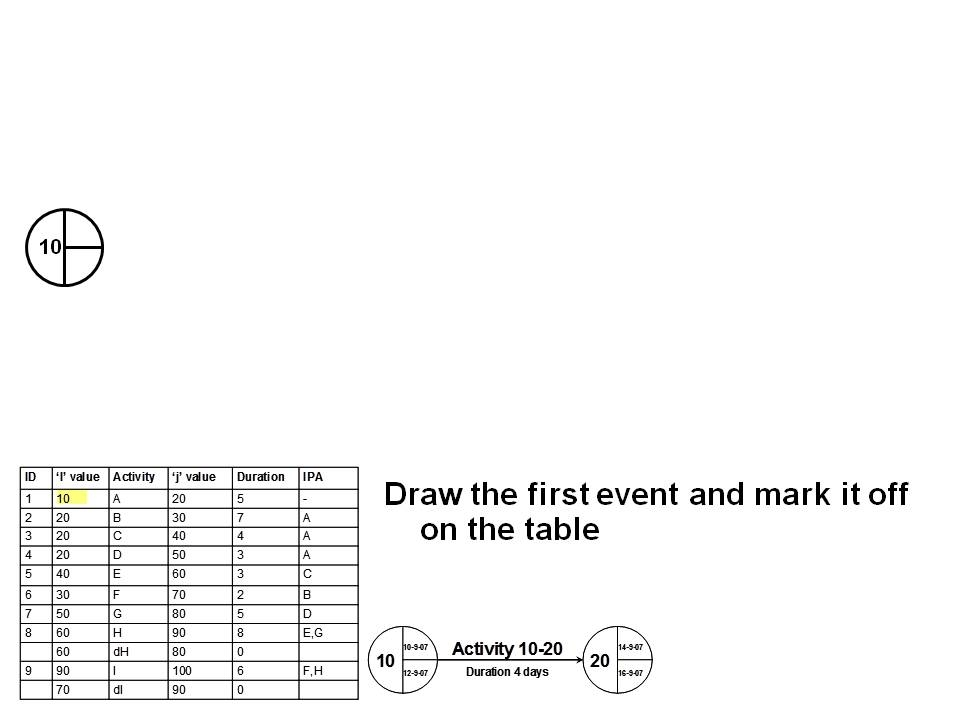
\includegraphics[width = 10.5cm]{oldnotes/Slide81.jpg}
\end{figure}
\end{frame}
\begin{center}\line(1,0){250}\end{center}


\begin{frame}
\begin{figure}
	\centering
		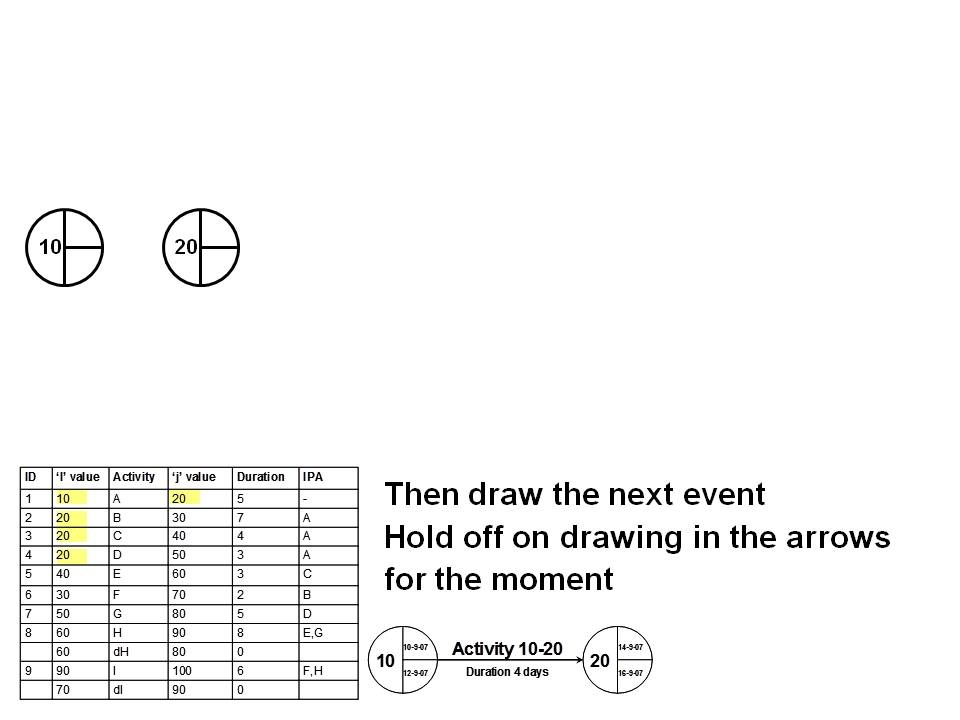
\includegraphics[width = 10.5cm]{oldnotes/Slide82.jpg}
\end{figure}
\end{frame}
\begin{center}\line(1,0){250}\end{center}


\begin{frame}
\begin{figure}
	\centering
		\includegraphics[width = 10.5cm]{oldnotes/Slide83.jpg}
\end{figure}
\end{frame}
\begin{center}\line(1,0){250}\end{center}


\begin{frame}
\begin{figure}
	\centering
		\includegraphics[width = 10.5cm]{oldnotes/Slide84.jpg}
\end{figure}
\end{frame}
\begin{center}\line(1,0){250}\end{center}


\begin{frame}
\begin{figure}
	\centering
		\includegraphics[width = 10.5cm]{oldnotes/Slide85.jpg}
\end{figure}
\end{frame}
\begin{center}\line(1,0){250}\end{center}


\begin{frame}
\begin{figure}
	\centering
		\includegraphics[width = 10.5cm]{oldnotes/Slide86.jpg}
\end{figure}
\end{frame}
\begin{center}\line(1,0){250}\end{center}


\begin{frame}
\begin{figure}
	\centering
		\includegraphics[width = 10.5cm]{oldnotes/Slide87.jpg}
\end{figure}
\end{frame}
\begin{center}\line(1,0){250}\end{center}


\begin{frame}
\begin{figure}
	\centering
		\includegraphics[width = 10.5cm]{oldnotes/Slide88.jpg}
\end{figure}
\end{frame}
\begin{center}\line(1,0){250}\end{center}


\begin{frame}
\begin{figure}
	\centering
		\includegraphics[width = 10.5cm]{oldnotes/Slide89.jpg}
\end{figure}
\end{frame}
\begin{center}\line(1,0){250}\end{center}


\begin{frame}
\begin{figure}
	\centering
		\includegraphics[width = 10.5cm]{oldnotes/Slide90.jpg}
\end{figure}
\end{frame}
\begin{center}\line(1,0){250}\end{center}


\begin{frame}
\begin{figure}
	\centering
		\includegraphics[width = 10.5cm]{oldnotes/Slide91.jpg}
\end{figure}
\end{frame}
\begin{center}\line(1,0){250}\end{center}


\begin{frame}
\begin{figure}
	\centering
		\includegraphics[width = 10.0cm]{oldnotes/Slide92.jpg}
\end{figure}
\end{frame}
\begin{center}\line(1,0){250}\end{center}


\begin{frame}
\begin{figure}
	\centering
		\includegraphics[width = 10.0cm]{oldnotes/Slide93.jpg}
\end{figure}
\end{frame}
\begin{center}\line(1,0){250}\end{center}


\begin{frame}
\begin{figure}
	\centering
		\includegraphics[width = 10.0cm]{oldnotes/Slide94.jpg}
\end{figure}
\end{frame}
\begin{center}\line(1,0){250}\end{center}


\begin{frame}
\begin{figure}
	\centering
		\includegraphics[width = 10.0cm]{oldnotes/Slide95.jpg}
\end{figure}
\end{frame}
\begin{center}\line(1,0){250}\end{center}


\begin{frame}
\begin{figure}
	\centering
		\includegraphics[width = 10.0cm]{oldnotes/Slide96.jpg}
\end{figure}
\end{frame}
\begin{center}\line(1,0){250}\end{center}


\begin{frame}
\begin{figure}
	\centering
		\includegraphics[width = 10.0cm]{oldnotes/Slide97.jpg}
\end{figure}
\end{frame}
\begin{center}\line(1,0){250}\end{center}


\begin{frame}
\begin{figure}
	\centering
		\includegraphics[width = 10.0cm]{oldnotes/Slide98.jpg}
\end{figure}
\end{frame}
\begin{center}\line(1,0){250}\end{center}


\begin{frame}
\begin{figure}
	\centering
		\includegraphics[width = 10.0cm]{oldnotes/Slide99.jpg}
\end{figure}
\end{frame}
\begin{center}\line(1,0){250}\end{center}


\begin{frame}
\begin{figure}
	\centering
		\includegraphics[width = 10.0cm]{oldnotes/Slide100.jpg}
\end{figure}
\end{frame}
\begin{center}\line(1,0){250}\end{center}


\begin{frame}
\begin{figure}
	\centering
		\includegraphics[width = 10.0cm]{oldnotes/Slide101.jpg}
\end{figure}
\end{frame}
\begin{center}\line(1,0){250}\end{center}


\begin{frame}
\begin{figure}
	\centering
		\includegraphics[width = 10.0cm]{oldnotes/Slide102.jpg}
\end{figure}
\end{frame}
\begin{center}\line(1,0){250}\end{center}


\begin{frame}
\begin{figure}
	\centering
		\includegraphics[width = 10.0cm]{oldnotes/Slide103.jpg}
\end{figure}
\end{frame}
\begin{center}\line(1,0){250}\end{center}


\begin{frame}
\begin{figure}
	\centering
		\includegraphics[width = 10.0cm]{oldnotes/Slide104.jpg}
\end{figure}
\end{frame}
\begin{center}\line(1,0){250}\end{center}


\begin{frame}
\begin{figure}
	\centering
		\includegraphics[width = 10.0cm]{oldnotes/Slide105.jpg}
\end{figure}
\end{frame}
\begin{center}\line(1,0){250}\end{center}


\begin{frame}
\begin{figure}
	\centering
		\includegraphics[width = 10.0cm]{oldnotes/Slide106.jpg}
\end{figure}
\end{frame}
\begin{center}\line(1,0){250}\end{center}


\begin{frame}
\begin{figure}
	\centering
		\includegraphics[width = 10.0cm]{oldnotes/Slide107.jpg}
\end{figure}
\end{frame}
\begin{center}\line(1,0){250}\end{center}


\begin{frame}
\begin{figure}
	\centering
		\includegraphics[width = 10.0cm]{oldnotes/Slide108.jpg}
\end{figure}
\end{frame}
\begin{center}\line(1,0){250}\end{center}


\begin{frame}
\begin{figure}
	\centering
		\includegraphics[width = 10.0cm]{oldnotes/Slide109.jpg}
\end{figure}
\end{frame}
\begin{center}\line(1,0){250}\end{center}


\begin{frame}
\begin{figure}
	\centering
		\includegraphics[width = 10.0cm]{oldnotes/Slide110.jpg}
\end{figure}
\end{frame}
\begin{center}\line(1,0){250}\end{center}


\begin{frame}
\begin{figure}
	\centering
		\includegraphics[width = 10.0cm]{oldnotes/Slide111.jpg}
\end{figure}
\end{frame}
\begin{center}\line(1,0){250}\end{center}


\begin{frame}
\begin{figure}
	\centering
		\includegraphics[width = 10.0cm]{oldnotes/Slide112.jpg}
\end{figure}
\end{frame}
\begin{center}\line(1,0){250}\end{center}


\begin{frame}
\begin{figure}
	\centering
		\includegraphics[width = 10.0cm]{oldnotes/Slide113.jpg}
\end{figure}
\end{frame}
\begin{center}\line(1,0){250}\end{center}


\begin{frame}
\begin{figure}
	\centering
		\includegraphics[width = 10.0cm]{oldnotes/Slide114.jpg}
\end{figure}
\end{frame}
\begin{center}\line(1,0){250}\end{center}


\begin{frame}
\begin{figure}
	\centering
		\includegraphics[width = 10.0cm]{oldnotes/Slide115.jpg}
\end{figure}
\end{frame}
\begin{center}\line(1,0){250}\end{center}


\begin{frame}
\begin{figure}
	\centering
		\includegraphics[width = 10.0cm]{oldnotes/Slide116.jpg}
\end{figure}
\end{frame}
\begin{center}\line(1,0){250}\end{center}


\begin{frame}
\begin{figure}
	\centering
		\includegraphics[width = 10.0cm]{oldnotes/Slide117.jpg}
\end{figure}
\end{frame}
\begin{center}\line(1,0){250}\end{center}


\begin{frame}
\begin{figure}
	\centering
		\includegraphics[width = 10.0cm]{oldnotes/Slide118.jpg}
\end{figure}
\end{frame}
\begin{center}\line(1,0){250}\end{center}


\begin{frame}
\begin{figure}
	\centering
		\includegraphics[width = 10.0cm]{oldnotes/Slide119.jpg}
\end{figure}
\end{frame}
\begin{center}\line(1,0){250}\end{center}


\begin{frame}
\begin{figure}
	\centering
		\includegraphics[width = 10.0cm]{oldnotes/Slide120.jpg}
\end{figure}
\end{frame}
\begin{center}\line(1,0){250}\end{center}


\begin{frame}
\begin{figure}
	\centering
		\includegraphics[width = 10.0cm]{oldnotes/Slide121.jpg}
\end{figure}
\end{frame}
\begin{center}\line(1,0){250}\end{center}


\begin{frame}
\begin{figure}
	\centering
		\includegraphics[width = 10.0cm]{oldnotes/Slide122.jpg}
\end{figure}
\end{frame}
\begin{center}\line(1,0){250}\end{center}



\section{Activity on Node}

\begin{frame}
\frametitle{Additional Resources}
\textbf{Support Material}\\
\href{https://sites.google.com/site/paulveseyresourcefiles/project-management/Lecture\%2011\%20-\%20Project\%20Time\%20Management\%20AON\%204-8.pptx?attredirects=0&d=1}{Powerpoint Download}\\
\href{https://docs.google.com/viewer?a=v&pid=sites&srcid=ZGVmYXVsdGRvbWFpbnxwYXVsdmVzZXlyZXNvdXJjZWZpbGVzfGd4OjNlMzYwYmNkOWEyNzhhOTM}{Powerpoint View Online}\\
\end{frame}
\begin{center}\line(1,0){250}\end{center}



\begin{frame}
\begin{figure}
	\centering
		\includegraphics[width = 10.0cm]{oldnotes/Slide124.jpg}
\end{figure}
\end{frame}
\begin{center}\line(1,0){250}\end{center}


\begin{frame}
\begin{figure}
	\centering
		\includegraphics[width = 10.0cm]{oldnotes/Slide125.jpg}
\end{figure}
\end{frame}
\begin{center}\line(1,0){250}\end{center}


\begin{frame}
\begin{figure}
	\centering
		\includegraphics[width = 10.0cm]{oldnotes/Slide126.jpg}
\end{figure}
\end{frame}
\begin{center}\line(1,0){250}\end{center}


\begin{frame}
\begin{figure}
	\centering
		\includegraphics[width = 10.0cm]{oldnotes/Slide127.jpg}
\end{figure}
\end{frame}
\begin{center}\line(1,0){250}\end{center}


\begin{frame}
\begin{figure}
	\centering
		\includegraphics[width = 10.0cm]{oldnotes/Slide128.jpg}
\end{figure}
\end{frame}
\begin{center}\line(1,0){250}\end{center}


\begin{frame}
\begin{figure}
	\centering
		\includegraphics[width = 10.0cm]{oldnotes/Slide129.jpg}
\end{figure}
\end{frame}
\begin{center}\line(1,0){250}\end{center}


\begin{frame}
\begin{figure}
	\centering
		\includegraphics[width = 10.0cm]{oldnotes/Slide130.jpg}
\end{figure}
\end{frame}
\begin{center}\line(1,0){250}\end{center}


\begin{frame}
\begin{figure}
	\centering
		\includegraphics[width = 10.0cm]{oldnotes/Slide131.jpg}
\end{figure}
\end{frame}
\begin{center}\line(1,0){250}\end{center}


\begin{frame}
\begin{figure}
	\centering
		\includegraphics[width = 10.0cm]{oldnotes/Slide132.jpg}
\end{figure}
\end{frame}
\begin{center}\line(1,0){250}\end{center}


\begin{frame}
\begin{figure}
	\centering
		\includegraphics[width = 10.0cm]{oldnotes/Slide133.jpg}
\end{figure}
\end{frame}
\begin{center}\line(1,0){250}\end{center}


\begin{frame}
\begin{figure}
	\centering
		\includegraphics[width = 10.0cm]{oldnotes/Slide134.jpg}
\end{figure}
\end{frame}
\begin{center}\line(1,0){250}\end{center}


\begin{frame}
\begin{figure}
	\centering
		\includegraphics[width = 10.0cm]{oldnotes/Slide135.jpg}
\end{figure}
\end{frame}
\begin{center}\line(1,0){250}\end{center}




\begin{frame}
\begin{figure}
	\centering
		\includegraphics[width = 10.0cm]{oldnotes/Slide136.jpg}
\end{figure}
\end{frame}
\begin{center}\line(1,0){250}\end{center}




\begin{frame}
\begin{figure}
	\centering
		\includegraphics[width = 10.0cm]{oldnotes/Slide137.jpg}
\end{figure}
\end{frame}
\begin{center}\line(1,0){250}\end{center}




\begin{frame}
\begin{figure}
	\centering
		\includegraphics[width = 10.0cm]{oldnotes/Slide138.jpg}
\end{figure}
\end{frame}
\begin{center}\line(1,0){250}\end{center}




\begin{frame}
\begin{figure}
	\centering
		\includegraphics[width = 10.0cm]{oldnotes/Slide139.jpg}
\end{figure}
\end{frame}
\begin{center}\line(1,0){250}\end{center}




\begin{frame}
\begin{figure}
	\centering
		\includegraphics[width = 10.0cm]{oldnotes/Slide140.jpg}
\end{figure}
\end{frame}
\begin{center}\line(1,0){250}\end{center}




\begin{frame}
\begin{figure}
	\centering
		\includegraphics[width = 10.0cm]{oldnotes/Slide141.jpg}
\end{figure}
\end{frame}
\begin{center}\line(1,0){250}\end{center}




\begin{frame}
\begin{figure}
	\centering
		\includegraphics[width = 10.0cm]{oldnotes/Slide142.jpg}
\end{figure}
\end{frame}
\begin{center}\line(1,0){250}\end{center}




\begin{frame}
\begin{figure}
	\centering
		\includegraphics[width = 10.0cm]{oldnotes/Slide143.jpg}
\end{figure}
\end{frame}
\begin{center}\line(1,0){250}\end{center}




\begin{frame}
\begin{figure}
	\centering
		\includegraphics[width = 10.0cm]{oldnotes/Slide144.jpg}
\end{figure}
\end{frame}
\begin{center}\line(1,0){250}\end{center}




\begin{frame}
\begin{figure}
	\centering
		\includegraphics[width = 10.0cm]{oldnotes/Slide145.jpg}
\end{figure}
\end{frame}
\begin{center}\line(1,0){250}\end{center}




\begin{frame}
\begin{figure}
	\centering
		\includegraphics[width = 10.0cm]{oldnotes/Slide146.jpg}
\end{figure}
\end{frame}
\begin{center}\line(1,0){250}\end{center}




\begin{frame}
\begin{figure}
	\centering
		\includegraphics[width = 10.0cm]{oldnotes/Slide147.jpg}
\end{figure}
\end{frame}
\begin{center}\line(1,0){250}\end{center}




\begin{frame}
\begin{figure}
	\centering
		\includegraphics[width = 10.0cm]{oldnotes/Slide148.jpg}
\end{figure}
\end{frame}
\begin{center}\line(1,0){250}\end{center}




\begin{frame}
\begin{figure}
	\centering
		\includegraphics[width = 10.0cm]{oldnotes/Slide149.jpg}
\end{figure}
\end{frame}
\begin{center}\line(1,0){250}\end{center}




\begin{frame}
\begin{figure}
	\centering
		\includegraphics[width = 10.0cm]{oldnotes/Slide150.jpg}
\end{figure}
\end{frame}
\begin{center}\line(1,0){250}\end{center}




\begin{frame}
\begin{figure}
	\centering
		\includegraphics[width = 10.0cm]{oldnotes/Slide151.jpg}
\end{figure}
\end{frame}
\begin{center}\line(1,0){250}\end{center}




\begin{frame}
\begin{figure}
	\centering
		\includegraphics[width = 10.0cm]{oldnotes/Slide152.jpg}
\end{figure}
\end{frame}
\begin{center}\line(1,0){250}\end{center}




\begin{frame}
\begin{figure}
	\centering
		\includegraphics[width = 10.0cm]{oldnotes/Slide153.jpg}
\end{figure}
\end{frame}
\begin{center}\line(1,0){250}\end{center}




\begin{frame}
\begin{figure}
	\centering
		\includegraphics[width = 10.0cm]{oldnotes/Slide154.jpg}
\end{figure}
\end{frame}
\begin{center}\line(1,0){250}\end{center}




\begin{frame}
\begin{figure}
	\centering
		\includegraphics[width = 10.0cm]{oldnotes/Slide155.jpg}
\end{figure}
\end{frame}
\begin{center}\line(1,0){250}\end{center}




\begin{frame}
\begin{figure}
	\centering
		\includegraphics[width = 10.0cm]{oldnotes/Slide156.jpg}
\end{figure}
\end{frame}
\begin{center}\line(1,0){250}\end{center}




\begin{frame}
\begin{figure}
	\centering
		\includegraphics[width = 10.0cm]{oldnotes/Slide157.jpg}
\end{figure}
\end{frame}
\begin{center}\line(1,0){250}\end{center}




\begin{frame}
\begin{figure}
	\centering
		\includegraphics[width = 10.0cm]{oldnotes/Slide158.jpg}
\end{figure}
\end{frame}
\begin{center}\line(1,0){250}\end{center}




\begin{frame}
\begin{figure}
	\centering
		\includegraphics[width = 10.0cm]{oldnotes/Slide159.jpg}
\end{figure}
\end{frame}
\begin{center}\line(1,0){250}\end{center}




\begin{frame}
\begin{figure}
	\centering
		\includegraphics[width = 10.0cm]{oldnotes/Slide160.jpg}
\end{figure}
\end{frame}
\begin{center}\line(1,0){250}\end{center}




\begin{frame}
\begin{figure}
	\centering
		\includegraphics[width = 10.0cm]{oldnotes/Slide161.jpg}
\end{figure}
\end{frame}
\begin{center}\line(1,0){250}\end{center}




\begin{frame}
\begin{figure}
	\centering
		\includegraphics[width = 10.0cm]{oldnotes/Slide162.jpg}
\end{figure}
\end{frame}
\begin{center}\line(1,0){250}\end{center}




\begin{frame}
\begin{figure}
	\centering
		\includegraphics[width = 10.0cm]{oldnotes/Slide163.jpg}
\end{figure}
\end{frame}
\begin{center}\line(1,0){250}\end{center}




\begin{frame}
\begin{figure}
	\centering
		\includegraphics[width = 10.0cm]{oldnotes/Slide164.jpg}
\end{figure}
\end{frame}
\begin{center}\line(1,0){250}\end{center}




\begin{frame}
\begin{figure}
	\centering
		\includegraphics[width = 10.0cm]{oldnotes/Slide165.jpg}
\end{figure}
\end{frame}
\begin{center}\line(1,0){250}\end{center}




\begin{frame}
\begin{figure}
	\centering
		\includegraphics[width = 10.0cm]{oldnotes/Slide166.jpg}
\end{figure}
\end{frame}
\begin{center}\line(1,0){250}\end{center}




\begin{frame}
\begin{figure}
	\centering
		\includegraphics[width = 10.0cm]{oldnotes/Slide167.jpg}
\end{figure}
\end{frame}
\begin{center}\line(1,0){250}\end{center}




\begin{frame}
\begin{figure}
	\centering
		\includegraphics[width = 10.0cm]{oldnotes/Slide168.jpg}
\end{figure}
\end{frame}
\begin{center}\line(1,0){250}\end{center}




\begin{frame}
\begin{figure}
	\centering
		\includegraphics[width = 10.0cm]{oldnotes/Slide169.jpg}
\end{figure}
\end{frame}
\begin{center}\line(1,0){250}\end{center}




\begin{frame}
\begin{figure}
	\centering
		\includegraphics[width = 10.0cm]{oldnotes/Slide170.jpg}
\end{figure}
\end{frame}
\begin{center}\line(1,0){250}\end{center}




\begin{frame}
\begin{figure}
	\centering
		\includegraphics[width = 10.0cm]{oldnotes/Slide171.jpg}
\end{figure}
\end{frame}
\begin{center}\line(1,0){250}\end{center}




\begin{frame}
\begin{figure}
	\centering
		\includegraphics[width = 10.0cm]{oldnotes/Slide172.jpg}
\end{figure}
\end{frame}
\begin{center}\line(1,0){250}\end{center}




\begin{frame}
\begin{figure}
	\centering
		\includegraphics[width = 10.0cm]{oldnotes/Slide173.jpg}
\end{figure}
\end{frame}
\begin{center}\line(1,0){250}\end{center}




\begin{frame}
\begin{figure}
	\centering
		\includegraphics[width = 10.0cm]{oldnotes/Slide174.jpg}
\end{figure}
\end{frame}
\begin{center}\line(1,0){250}\end{center}




\begin{frame}
\begin{figure}
	\centering
		\includegraphics[width = 10.0cm]{oldnotes/Slide175.jpg}
\end{figure}
\end{frame}
\begin{center}\line(1,0){250}\end{center}




\begin{frame}
\begin{figure}
	\centering
		\includegraphics[width = 10.0cm]{oldnotes/Slide176.jpg}
\end{figure}
\end{frame}
\begin{center}\line(1,0){250}\end{center}




\begin{frame}
\begin{figure}
	\centering
		\includegraphics[width = 10.0cm]{oldnotes/Slide177.jpg}
\end{figure}
\end{frame}
\begin{center}\line(1,0){250}\end{center}




\begin{frame}
\begin{figure}
	\centering
		\includegraphics[width = 10.0cm]{oldnotes/Slide178.jpg}
\end{figure}
\end{frame}
\begin{center}\line(1,0){250}\end{center}




\begin{frame}
\begin{figure}
	\centering
		\includegraphics[width = 10.0cm]{oldnotes/Slide179.jpg}
\end{figure}
\end{frame}
\begin{center}\line(1,0){250}\end{center}




\begin{frame}
\begin{figure}
	\centering
		\includegraphics[width = 10.0cm]{oldnotes/Slide180.jpg}
\end{figure}
\end{frame}
\begin{center}\line(1,0){250}\end{center}




\begin{frame}
\begin{figure}
	\centering
		\includegraphics[width = 10.0cm]{oldnotes/Slide181.jpg}
\end{figure}
\end{frame}
\begin{center}\line(1,0){250}\end{center}




\begin{frame}
\begin{figure}
	\centering
		\includegraphics[width = 10.0cm]{oldnotes/Slide182.jpg}
\end{figure}
\end{frame}
\begin{center}\line(1,0){250}\end{center}




\begin{frame}
\begin{figure}
	\centering
		\includegraphics[width = 10.0cm]{oldnotes/Slide183.jpg}
\end{figure}
\end{frame}
\begin{center}\line(1,0){250}\end{center}




\begin{frame}
\begin{figure}
	\centering
		\includegraphics[width = 10.0cm]{oldnotes/Slide184.jpg}
\end{figure}
\end{frame}
\begin{center}\line(1,0){250}\end{center}




\begin{frame}
\begin{figure}
	\centering
		\includegraphics[width = 10.0cm]{oldnotes/Slide185.jpg}
\end{figure}
\end{frame}
\begin{center}\line(1,0){250}\end{center}




\begin{frame}
\begin{figure}
	\centering
		\includegraphics[width = 10.0cm]{oldnotes/Slide186.jpg}
\end{figure}
\end{frame}
\begin{center}\line(1,0){250}\end{center}




\begin{frame}
\begin{figure}
	\centering
		\includegraphics[width = 10.0cm]{oldnotes/Slide187.jpg}
\end{figure}
\end{frame}
\begin{center}\line(1,0){250}\end{center}




\begin{frame}
\begin{figure}
	\centering
		\includegraphics[width = 10.0cm]{oldnotes/Slide188.jpg}
\end{figure}
\end{frame}
\begin{center}\line(1,0){250}\end{center}




\begin{frame}
\begin{figure}
	\centering
		\includegraphics[width = 10.0cm]{oldnotes/Slide189.jpg}
\end{figure}
\end{frame}
\begin{center}\line(1,0){250}\end{center}




\begin{frame}
\begin{figure}
	\centering
		\includegraphics[width = 10.0cm]{oldnotes/Slide190.jpg}
\end{figure}
\end{frame}
\begin{center}\line(1,0){250}\end{center}




\begin{frame}
\begin{figure}
	\centering
		\includegraphics[width = 10.0cm]{oldnotes/Slide191.jpg}
\end{figure}
\end{frame}
\begin{center}\line(1,0){250}\end{center}




\begin{frame}
\begin{figure}
	\centering
		\includegraphics[width = 10.0cm]{oldnotes/Slide192.jpg}
\end{figure}
\end{frame}
\begin{center}\line(1,0){250}\end{center}




\begin{frame}
\begin{figure}
	\centering
		\includegraphics[width = 10.0cm]{oldnotes/Slide193.jpg}
\end{figure}
\end{frame}
\begin{center}\line(1,0){250}\end{center}




\begin{frame}
\begin{figure}
	\centering
		\includegraphics[width = 10.0cm]{oldnotes/Slide194.jpg}
\end{figure}
\end{frame}
\begin{center}\line(1,0){250}\end{center}




\begin{frame}
\begin{figure}
	\centering
		\includegraphics[width = 10.0cm]{oldnotes/Slide195.jpg}
\end{figure}
\end{frame}
\begin{center}\line(1,0){250}\end{center}




\begin{frame}
\begin{figure}
	\centering
		\includegraphics[width = 10.0cm]{oldnotes/Slide196.jpg}
\end{figure}
\end{frame}
\begin{center}\line(1,0){250}\end{center}




\begin{frame}
\begin{figure}
	\centering
		\includegraphics[width = 10.0cm]{oldnotes/Slide197.jpg}
\end{figure}
\end{frame}
\begin{center}\line(1,0){250}\end{center}




\begin{frame}
\begin{figure}
	\centering
		\includegraphics[width = 10.0cm]{oldnotes/Slide198.jpg}
\end{figure}
\end{frame}
\begin{center}\line(1,0){250}\end{center}




\begin{frame}
\begin{figure}
	\centering
		\includegraphics[width = 10.0cm]{oldnotes/Slide199.jpg}
\end{figure}
\end{frame}
\begin{center}\line(1,0){250}\end{center}




\begin{frame}
\begin{figure}
	\centering
		\includegraphics[width = 10.0cm]{oldnotes/Slide200.jpg}
\end{figure}
\end{frame}
\begin{center}\line(1,0){250}\end{center}




\begin{frame}
\begin{figure}
	\centering
		\includegraphics[width = 10.0cm]{oldnotes/Slide201.jpg}
\end{figure}
\end{frame}
\begin{center}\line(1,0){250}\end{center}




\begin{frame}
\begin{figure}
	\centering
		\includegraphics[width = 10.0cm]{oldnotes/Slide202.jpg}
\end{figure}
\end{frame}
\begin{center}\line(1,0){250}\end{center}




\begin{frame}
\begin{figure}
	\centering
		\includegraphics[width = 10.0cm]{oldnotes/Slide203.jpg}
\end{figure}
\end{frame}
\begin{center}\line(1,0){250}\end{center}




\begin{frame}
\begin{figure}
	\centering
		\includegraphics[width = 10.0cm]{oldnotes/Slide204.jpg}
\end{figure}
\end{frame}
\begin{center}\line(1,0){250}\end{center}




\begin{frame}
\begin{figure}
	\centering
		\includegraphics[width = 10.0cm]{oldnotes/Slide205.jpg}
\end{figure}
\end{frame}
\begin{center}\line(1,0){250}\end{center}




\begin{frame}
\begin{figure}
	\centering
		\includegraphics[width = 10.0cm]{oldnotes/Slide206.jpg}
\end{figure}
\end{frame}
\begin{center}\line(1,0){250}\end{center}




\begin{frame}
\begin{figure}
	\centering
		\includegraphics[width = 10.0cm]{oldnotes/Slide207.jpg}
\end{figure}
\end{frame}
\begin{center}\line(1,0){250}\end{center}




\begin{frame}
\begin{figure}
	\centering
		\includegraphics[width = 10.0cm]{oldnotes/Slide208.jpg}
\end{figure}
\end{frame}
\begin{center}\line(1,0){250}\end{center}




\begin{frame}
\begin{figure}
	\centering
		\includegraphics[width = 10.0cm]{oldnotes/Slide209.jpg}
\end{figure}
\end{frame}
\begin{center}\line(1,0){250}\end{center}




\begin{frame}
\begin{figure}
	\centering
		\includegraphics[width = 10.0cm]{oldnotes/Slide210.jpg}
\end{figure}
\end{frame}
\begin{center}\line(1,0){250}\end{center}




\begin{frame}
\begin{figure}
	\centering
		\includegraphics[width = 10.0cm]{oldnotes/Slide211.jpg}
\end{figure}
\end{frame}
\begin{center}\line(1,0){250}\end{center}




\begin{frame}
\begin{figure}
	\centering
		\includegraphics[width = 10.0cm]{oldnotes/Slide212.jpg}
\end{figure}
\end{frame}
\begin{center}\line(1,0){250}\end{center}




\begin{frame}
\begin{figure}
	\centering
		\includegraphics[width = 10.0cm]{oldnotes/Slide213.jpg}
\end{figure}
\end{frame}
\begin{center}\line(1,0){250}\end{center}




\begin{frame}
\begin{figure}
	\centering
		\includegraphics[width = 10.0cm]{oldnotes/Slide214.jpg}
\end{figure}
\end{frame}
\begin{center}\line(1,0){250}\end{center}




\begin{frame}
\begin{figure}
	\centering
		\includegraphics[width = 10.0cm]{oldnotes/Slide215.jpg}
\end{figure}
\end{frame}
\begin{center}\line(1,0){250}\end{center}




\begin{frame}
\begin{figure}
	\centering
		\includegraphics[width = 10.0cm]{oldnotes/Slide216.jpg}
\end{figure}
\end{frame}
\begin{center}\line(1,0){250}\end{center}




\begin{frame}
\begin{figure}
	\centering
		\includegraphics[width = 10.0cm]{oldnotes/Slide217.jpg}
\end{figure}
\end{frame}
\begin{center}\line(1,0){250}\end{center}




\begin{frame}
\begin{figure}
	\centering
		\includegraphics[width = 10.0cm]{oldnotes/Slide218.jpg}
\end{figure}
\end{frame}
\begin{center}\line(1,0){250}\end{center}




\begin{frame}
\begin{figure}
	\centering
		\includegraphics[width = 10.0cm]{oldnotes/Slide219.jpg}
\end{figure}
\end{frame}
\begin{center}\line(1,0){250}\end{center}




\begin{frame}
\begin{figure}
	\centering
		\includegraphics[width = 10.0cm]{oldnotes/Slide220.jpg}
\end{figure}
\end{frame}
\begin{center}\line(1,0){250}\end{center}




\begin{frame}
\begin{figure}
	\centering
		\includegraphics[width = 10.0cm]{oldnotes/Slide221.jpg}
\end{figure}
\end{frame}
\begin{center}\line(1,0){250}\end{center}




\begin{frame}
\begin{figure}
	\centering
		\includegraphics[width = 10.0cm]{oldnotes/Slide222.jpg}
\end{figure}
\end{frame}
\begin{center}\line(1,0){250}\end{center}




\begin{frame}
\begin{figure}
	\centering
		\includegraphics[width = 10.0cm]{oldnotes/Slide223.jpg}
\end{figure}
\end{frame}
\begin{center}\line(1,0){250}\end{center}




\begin{frame}
\begin{figure}
	\centering
		\includegraphics[width = 10.0cm]{oldnotes/Slide224.jpg}
\end{figure}
\end{frame}
\begin{center}\line(1,0){250}\end{center}




\begin{frame}
\begin{figure}
	\centering
		\includegraphics[width = 10.0cm]{oldnotes/Slide225.jpg}
\end{figure}
\end{frame}
\begin{center}\line(1,0){250}\end{center}




\begin{frame}
\begin{figure}
	\centering
		\includegraphics[width = 10.0cm]{oldnotes/Slide226.jpg}
\end{figure}
\end{frame}
\begin{center}\line(1,0){250}\end{center}




\begin{frame}
\begin{figure}
	\centering
		\includegraphics[width = 10.0cm]{oldnotes/Slide227.jpg}
\end{figure}
\end{frame}
\begin{center}\line(1,0){250}\end{center}




\begin{frame}
\begin{figure}
	\centering
		\includegraphics[width = 10.0cm]{oldnotes/Slide228.jpg}
\end{figure}
\end{frame}
\begin{center}\line(1,0){250}\end{center}




\begin{frame}
\begin{figure}
	\centering
		\includegraphics[width = 10.0cm]{oldnotes/Slide229.jpg}
\end{figure}
\end{frame}
\begin{center}\line(1,0){250}\end{center}




\begin{frame}
\begin{figure}
	\centering
		\includegraphics[width = 10.0cm]{oldnotes/Slide230.jpg}
\end{figure}
\end{frame}
\begin{center}\line(1,0){250}\end{center}




\begin{frame}
\begin{figure}
	\centering
		\includegraphics[width = 10.0cm]{oldnotes/Slide231.jpg}
\end{figure}
\end{frame}
\begin{center}\line(1,0){250}\end{center}




\begin{frame}
\begin{figure}
	\centering
		\includegraphics[width = 10.0cm]{oldnotes/Slide232.jpg}
\end{figure}
\end{frame}
\begin{center}\line(1,0){250}\end{center}




\begin{frame}
\begin{figure}
	\centering
		\includegraphics[width = 10.0cm]{oldnotes/Slide233.jpg}
\end{figure}
\end{frame}
\begin{center}\line(1,0){250}\end{center}




\begin{frame}
\begin{figure}
	\centering
		\includegraphics[width = 10.0cm]{oldnotes/Slide234.jpg}
\end{figure}
\end{frame}
\begin{center}\line(1,0){250}\end{center}




\begin{frame}
\begin{figure}
	\centering
		\includegraphics[width = 10.0cm]{oldnotes/Slide235.jpg}
\end{figure}
\end{frame}
\begin{center}\line(1,0){250}\end{center}




\begin{frame}
\begin{figure}
	\centering
		\includegraphics[width = 10.0cm]{oldnotes/Slide236.jpg}
\end{figure}
\end{frame}
\begin{center}\line(1,0){250}\end{center}




\begin{frame}
\begin{figure}
	\centering
		\includegraphics[width = 10.0cm]{oldnotes/Slide237.jpg}
\end{figure}
\end{frame}
\begin{center}\line(1,0){250}\end{center}




\begin{frame}
\begin{figure}
	\centering
		\includegraphics[width = 10.0cm]{oldnotes/Slide238.jpg}
\end{figure}
\end{frame}
\begin{center}\line(1,0){250}\end{center}




\begin{frame}
\begin{figure}
	\centering
		\includegraphics[width = 10.0cm]{oldnotes/Slide239.jpg}
\end{figure}
\end{frame}
\begin{center}\line(1,0){250}\end{center}




\begin{frame}
\begin{figure}
	\centering
		\includegraphics[width = 10.0cm]{oldnotes/Slide240.jpg}
\end{figure}
\end{frame}
\begin{center}\line(1,0){250}\end{center}


\section{PERT}






\begin{frame}
\frametitle{PERT}
Program Evaluation \& Review Technique
\end{frame}
\begin{center}\line(1,0){250}\end{center}





\begin{frame}
\frametitle{What is PERT?}
Program Evaluation and Review Technique
\begin{itemize}
	\item Event Orientated Network Analysis
	\item Used where individual activity durations are highly uncertain
	\item PERT applies weighted average duration estimates to the Critical Path Method (CPM)
	\item PERT is a probabilistic or stochastic method
\end{itemize}
\end{frame}
\begin{center}\line(1,0){250}\end{center}




\begin{frame}
\frametitle{History of PERT}
1950's - US Navy had huge cost overruns on the Polaris Missile System Project, primarily due to the lack of historical data.\\
The project team (USN, Lockheed, Allen Hamilton) began to research effort to develop a tool to assist the planning of the Polaris Project.\\
Objective was to devise a method that can predict a completion date and assign a probability to meeting that date.\\
June 1962; Department of Defence and NASA officially adopt system.\\
\end{frame}
\begin{center}\line(1,0){250}\end{center}



\begin{frame}
\frametitle{Concept of PERT}
PERT is a probabilistic approach that requires a duration frequency distribution for each activity.\\
Each Activity is given:\\
\begin{itemize}
	\item $T_O$ - Optimistic Duration
	\item $T_M$ - Most Likely Duration
	\item $T_P$ - Pessimistic Duration
\end{itemize}
Paint Room, expect 3 days, maybe 2, but could be 5 days if paint runs out.
\begin{itemize}
	\item $T_O$ = 2 days; $T_M$ = 3 days; $T_P$ = 5 days;
\end{itemize}
\end{frame}
\begin{center}\line(1,0){250}\end{center}



\begin{frame}
\frametitle{Concept of PERT}
These 3 durations give a `distribution' for the activity, therefore we can produce a statistical mean and variance for the duration of the activity.\\
PERT treats the means of these activity durations as a normal distribution, and then using normal statistical methods, a mean duration, and variance (or standard deviation) of the time required to complete the chain of activities. \\
The result is that completion can be calculated as a  probability that it will occur by a particular day.\\
\end{frame}
\begin{center}\line(1,0){250}\end{center}



\begin{frame}
\frametitle{Mathematics of PERT}
The Mean Weighted Average of these three durations is called the Expected Duration $T_e$

\begin{equation}
T_e = \frac{T_o + 4T_m + T_p}{6} \label{eqn:waverage} \tag{PERT-1}	
\end{equation}


Where:\\	
\begin{itemize}
	\item $T_o$ is the Optimistic Duration
	\item $T_m$ is the Most Likely Duration
	\item $T_p$ is the Pessimistic Duration
	\item $T_e$ is the Expected Duration
\end{itemize}
\end{frame}
\begin{center}\line(1,0){250}\end{center}
In order to avoid confusion when referring to the entire path or the individual tasks, uppercase letters are used to refer to the entire path i.e. $T_E$, and lowercase letters are used to refer to the individual tasks, i.e. $T_e$


\begin{frame}
\frametitle{Mathematics of PERT}
Values for $T_o$ ,$T_m$ and $T_p$, are determined through experience, judgement, knowledge etc.\\
The weights assigned to $T_o$ ,$T_m$  and $T_p$ can be adjusted; however the denominator of Eqn. \eqref{eqn:waverage} must equal the sum of the weights.  i.e. $1+4+1 = 6$ \\
This arithmetic average is sometimes referred to as $\mu$ or $\overline{X}$
\end{frame}
\begin{center}\line(1,0){250}\end{center}



\begin{frame}
\frametitle{Mathematics of PERT}
The standard deviation (SD) of the expected duration is:\\
\begin{equation}
\sigma = \frac{T_{p}-T_{o}}{6} \label{eqn:sd} \tag{PERT-2}
\end{equation}

The variance ($V_e$)is given by:\\
\begin{equation}
V_e = \sigma_{e}^2 \label{eqn:var} \tag{PERT-3}
\end{equation}

\end{frame}
\begin{center}\line(1,0){250}\end{center}




\begin{frame}
\frametitle{Mathematics of PERT}
Now, add the expected durations for all activities on the studied path ($T_E$):\\
\begin{equation}
T_{E} = \sum\limits_{i=1}^{n}(T_{e})i \label{eqn:sumTe} \tag{PERT-4}
\end{equation}

Following on, the Variance ($V_E$) for the entire path can be calculated from:\\
\begin{equation}
V_E = \sum\limits_{i=1}^{n}(\sigma_{e}^{2})i \label{eqn:sumSD} \tag{PERT-5}
\end{equation}
\end{frame}
\begin{center}\line(1,0){250}\end{center}



\begin{frame}
\frametitle{Mathematics of PERT}
And the Standard Deviation ($\sigma_E$) for the entire path can be calculated from:


\begin{equation}
\sigma_E =\sqrt{V_E} \label{eqn:rootvar} \tag{PERT-6}
\end{equation}


\end{frame}
\begin{center}\line(1,0){250}\end{center}



\begin{frame}
\frametitle{Mathematics of PERT}
Using the previous calculations, it is possible to calculate the probability that a certain event will occur on or by a certain date ($T_S$) by using the normal distribution formulas:


\begin{equation}
Z =\frac{T_{S}-T_{E}}{\sigma_E} \label{eqn:zeqn} \tag{PERT-7}
\end{equation}
Where Z (called the Z function) represents the standard deviations ($\sigma_E$) away from the mean ($T_E$)

By rearranging Eqn. PERT-7 we can obtain an equation that will predict the date by which completion will occur with a known level of confidence (probability). \\
\begin{equation}
T_{S} =\sigma_{E}Z+T_{E} \label{eqn:zflat} \tag{PERT-8}
\end{equation}


\end{frame}
\begin{center}\line(1,0){250}\end{center}
You will be expected to remember these equations.  The second equation is simply a rearrengement of the first.

\begin{equation}
Z =\frac{T_{S}-T_{E}}{\sigma_E} 
\end{equation}
bring up $\sigma_E$ \notag
\begin{equation}
\sigma_{E}Z =T_{S}-T_{E} \notag
\end{equation}
bring over $T_E$
\begin{equation}
\sigma_{E}Z + T_{E} = T_{S} \notag
\end{equation}
and swapping sides:

\begin{equation}
 T_{S} =\sigma_{E}Z + T_{E} \notag
\end{equation}


\subsection{Example}

\begin{frame}
\frametitle{PERT Calculations}
Example:\\
By using the Critical Path Method (CPM) the following critical path has been determined.


\begin{table}
	\centering
		\begin{tabular}{|c|c|c|c|}
		\hline
		Activity 	& 	Optimistic 		 & 	Most Likely  	& 	Pessimistic \\
			  		&	Duration ($T_o$) &	Duration ($T_m$)&	Duration ($T_P$)\\
		\hline
		A & 2 & 4 & 7 \\		
		C & 5 & 8 & 14 \\
		F & 4 & 6 & 8 \\
		J & 2 & 2 & 2 \\
		K & 7 & 10 & 21 \\
		\hline
		\end{tabular}
\end{table}
\end{frame}
\begin{center}\line(1,0){250}\end{center}



\begin{frame}
\frametitle{PERT Calculations}
Example (cont.)
Calculate the following Values:
\begin{enumerate}
	\item The probability that the project will finish by the end of day 32
	\item The probability that the project will finish by the end of day 34
	\item The probability that the project will finish before day 30
	\item The probability that the project will finish on the 32nd day
	\item The probability that the project will finish no later than the 35th day
	\item The probability that the project will finish at least 2 days early
	\item The probability that the project will finish at least 2 days late
	\item The probability that the project will finish on the 32nd day  $\pm$1 day
	\item The completion date with at least 90\% confidence level
\end{enumerate}



\end{frame}
\begin{center}\line(1,0){250}\end{center}



\begin{frame}
\frametitle{PERT Calculations}
Example (cont.)\\
Before going any further, we need to calculate the expected duration ($T_E$) and the standard deviation ($\sigma_E$) of the path ACFJK.\\
So, for every activity we calculate the expected duration ($T_e$) and the standard deviation ($\sigma_e$) by using equations \eqref{eqn:waverage} and \eqref{eqn:sd}.
	
\begin{table}
	\centering
	\scalebox{0.6}{
		\begin{tabular}{|c|c|c|c|c|c|c|}
		\hline
		Activity 	& 	Optimistic 		 & 	Most Likely  	& 	Pessimistic 		&	Expected	&	Std. Dev	&	Variance	\\
			  		&	Duration ($T_o$) &	Duration ($T_m$)&	Duration ($T_P$)	&	Duration	&	$\sigma_{e}$&	$V_{e} = \sigma_{e}^{2}$	\\
		\hline
		A 			& 2 & 4  & 7 	&	4.167	&	0.833	&	0.694	\\		
		C 			& 5 & 8  & 14 	&	8.500	&	1.500	&	2.250	\\
		F 			& 4 & 6  & 8 	&	6.000	&	0.667	&	0.444	\\
		J 			& 2 & 2  & 2 	&	2.000	&	0.000	&	0.000	\\
		K 			& 7 & 10 & 21 	&	11.333	&	2.333	&	5.444	\\
		\hline \hline
		 			&  	&  	 &		&	$T_E = $ \textbf{32.000}	&		&	$V_E = $\textbf{8.833}\\
		\hline
		\end{tabular}}
\end{table}	
\end{frame}
\begin{center}\line(1,0){250}\end{center}
NOTE: When you are doing these calculation make sure you work to 3 places of decimal.  These calculations are very sensitive, particularly when $\sigma_{E}$ is small, i.e. less than 2.0.


\begin{frame}
\frametitle{PERT Calculations}
Now that we have determined:\\
$T_E$ = 32.000 days\\
$V_E$ = 8.833 days\\
we can calculate the standard deviation of the entire path ($\sigma_E$) from:\\
\begin{equation}
\sigma_{E} = \sqrt{V_{E}} \notag
\end{equation}

to give:
\begin{center}
		 $\sigma_{E}= $2.972 days
\end{center}

\end{frame}
\begin{center}\line(1,0){250}\end{center}



\begin{frame}
\frametitle{PERT Calculations Example 1}
\textit{The probability that the project will finish by the end of day 32.}\\
Z is calculated using Eqn \eqref{eqn:zeqn}.  For this case $T_S=32$, so inserting the values we get 

\begin{columns}
  \begin{column}{0.6\textwidth}
  
		\begin{equation}
		Z =\frac{T_{S}-T_{E}}{\sigma_E} =\frac{32-32}{2.972} = 0.000 \notag
		\end{equation}
  
    We then need to look-up the Z-tables at value 0.00 \\
	From the table we can see that the probability that the project will complete on day 32	is 0.50 or 50\%
  \end{column}
  \begin{column}{0.4\textwidth}
 
 
 		\begin{table}
			\centering
 			\scalebox{0.5}{			
				\begin{tabular}{|c|c|c|c|}
						\hline
						Z 	&	0.00	&	0.01	&	0.02	\\
						\hline
						0.0	&	0.5000	&	0.5040	&	0.5080	\\
						0.1	&	0.5398	&	0.5438	&	0.5478	\\
						0.2	&	0.5793	&	0.5832	&	0.5871	\\
						\hline	
				\end{tabular}}
		\end{table}
 
 
 
\begin{center}
  		\scalebox{0.5}{
	    \begin{tikzpicture}
		\begin{axis}[
		    samples=100,
		    domain=20:45, 
		    xmin=20,xmax=45,ymin=0,ymax=.15,
		    restrict y to domain=0:0.7,
		    extra x ticks={32},
		    extra x tick style={grid=major, tick label style={thick,rotate=90,anchor=east}},
		    extra x tick labels={$T_{E}=32$},
		    axis lines=left,
			ymajorgrids=true,
			xmajorgrids=true,
		    xtick={20,25,30,35,40},
		    minor x tick num =4,
		    ytick={0,0.10},
		    compat=newest,
		    xlabel=End of Day, xlabel style={at={(1,0)}, anchor=west},
		    ylabel=$P$, ylabel style={rotate=-90,at={(0,1)}, anchor=south}
		    ]
		    \addplot[domain=22:32, fill=lightgray] {(1/(2.972*(2*3.1415926535)^(0.5)))*(exp(0-((((x-32))^2)/(2*(2.972^2)))))}\closedcycle;           
		    \addplot[domain=22:43, red, ultra thick] {(1/(2.972*(2*3.1415926535)^(0.5)))*(exp(0-((((x-32))^2)/(2*(2.972^2)))))};
		%    \draw[->,color=blue] (32,0) -- (32,0.15);
		    \addplot[red, dashed] coordinates {(32, 0.0) (32, 0.15)};
		\end{axis}
		\end{tikzpicture}}
\end{center}
		
 

		
		
		
		  \end{column}
\end{columns}
\end{frame}
\begin{center}\line(1,0){250}\end{center}









\begin{frame}
\frametitle{PERT Calculations Example 2}
\textit{The probability that the project will finish by the end of day 34}\\
Z is calculated using Eqn \eqref{eqn:zeqn}.  For this case $T_S=34$, so inserting the values we get: 

\begin{columns}
  \begin{column}{0.6\textwidth}
  
		\begin{equation}
		Z =\frac{T_{S}-T_{E}}{\sigma_E} =\frac{34-32}{2.972} = 0.672 \notag
		\end{equation}
  
    We then need to look-up the Z-tables at value 0.67 \\
	From the table we can see that the probability that the	project will complete by the end of day 34 is 0.7486 or 74.9\%
  \end{column}
  \begin{column}{0.4\textwidth}
 
 
 		\begin{table}
			\centering
 			\scalebox{0.5}{			
				\begin{tabular}{|c|c|c|c|}
						\hline
						Z 	&	0.06	&	0.07	&	0.08	\\
						\hline
						0.5	&	0.7123	&	0.7157	&	0.719	\\
						0.6	&	0.7454	&	0.7486	&	0.7517	\\
						0.7	&	0.7764	&	0.7794	&	0.7823	\\
						\hline	
				\end{tabular}}
		\end{table}
 
 
 
\begin{center}
  		\scalebox{0.5}{
	    \begin{tikzpicture}
		\begin{axis}[
		    samples=100,
		    domain=20:45, 
		    xmin=20,xmax=45,ymin=0,ymax=.15,
		    restrict y to domain=0:0.7,
		    extra x ticks={32},
		    extra x tick style={grid=major, tick label style={thick,rotate=90,anchor=east}},
		    extra x tick labels={$T_{E}=32$},
		    axis lines=left,
			ymajorgrids=true,
			xmajorgrids=true,
		    xtick={20,25,30,35,40},
		    minor x tick num =4,
		    ytick={0,0.10},
		    compat=newest,
		    xlabel=End of Day, xlabel style={at={(1,0)}, anchor=west},
		    ylabel=$P$, ylabel style={rotate=-90,at={(0,1)}, anchor=south}
		    ]
		    \addplot[domain=22:34, fill=lightgray] {(1/(2.972*(2*3.1415926535)^(0.5)))*(exp(0-((((x-32))^2)/(2*(2.972^2)))))}\closedcycle;           
		    \addplot[domain=22:43, red, ultra thick] {(1/(2.972*(2*3.1415926535)^(0.5)))*(exp(0-((((x-32))^2)/(2*(2.972^2)))))};
		%    \draw[->,color=blue] (32,0) -- (32,0.15);
		    \addplot[red, dashed] coordinates {(32, 0.0) (32, 0.15)};
		\end{axis}
		\end{tikzpicture}}
\end{center}
		
 

		
		
		
		  \end{column}
\end{columns}



\end{frame}
\begin{center}\line(1,0){250}\end{center}



\begin{frame}
\frametitle{PERT Calculations Example 3}
\textit{The probability that the project will finish before day 30}\\
Note: this is the same as the probability of finishing by the end of day 29, so $T_S=29$. 


\begin{columns}
  \begin{column}{0.6\textwidth}
  
		\begin{equation}
		Z =\frac{29-32}{2.972} =\frac{-3}{2.972} = -1.009 \notag
		\end{equation}
In this case Z is less than Zero.  For values of Z less than zero, lookup the absolute value of Z as derived, and subtract from 1.00\\ 
So, subtracting 0.8438 from 1 we get 0.1562 or 15.6\%
  \end{column}
  \begin{column}{0.4\textwidth}
 
 
 		\begin{table}
			\centering
 			\scalebox{0.5}{			
				\begin{tabular}{|c|c|c|c|}
						\hline
						Z 	&	0	&	0.01	&	0.02	\\
						\hline
						0.9	&	0.8159	&	0.8186	&	0.8212	\\
						1	&	0.8413	&	0.8438	&	0.8461	\\
						1.1	&	0.8643	&	0.8665	&	0.8686	\\
						\hline	
				\end{tabular}}
		\end{table}
 
 
 
\begin{center}
  		\scalebox{0.5}{
	    \begin{tikzpicture}
		\begin{axis}[
		    samples=100,
		    domain=20:45, 
		    xmin=20,xmax=45,ymin=0,ymax=.15,
		    restrict y to domain=0:0.7,
		    extra x ticks={32},
		    extra x tick style={grid=major, tick label style={thick,rotate=90,anchor=east}},
		    extra x tick labels={$T_{E}=32$},
		    axis lines=left,
			ymajorgrids=true,
			xmajorgrids=true,
		    xtick={20,25,30,35,40},
		    minor x tick num =4,
		    ytick={0,0.10},
		    compat=newest,
		    xlabel=End of Day, xlabel style={at={(1,0)}, anchor=west},
		    ylabel=$P$, ylabel style={rotate=-90,at={(0,1)}, anchor=south}
		    ]
		    \addplot[domain=22:29, fill=lightgray] {(1/(2.972*(2*3.1415926535)^(0.5)))*(exp(0-((((x-32))^2)/(2*(2.972^2)))))}\closedcycle;           
		    \addplot[domain=22:43, red, ultra thick] {(1/(2.972*(2*3.1415926535)^(0.5)))*(exp(0-((((x-32))^2)/(2*(2.972^2)))))};
		%    \draw[->,color=blue] (32,0) -- (32,0.15);
		    \addplot[red, dashed] coordinates {(32, 0.0) (32, 0.15)};
		\end{axis}
		\end{tikzpicture}}
\end{center}
		
		  \end{column}
\end{columns}

\end{frame}
\begin{center}\line(1,0){250}\end{center}



\begin{frame}
\frametitle{PERT Calculations Example 4}
\textit{The probability that the project will finish on the 32nd day}\\
From part 1. we have already calculated the probability that the project will finish by the end of day 32.  i.e. Pr($T_{S}\leq32$)=0.50 or 50\%, so now we need to calculate Pr($T_{S}\leq31$).

	Pr($T_{S}\leq31$) = 1 - 0.633 = 0.367 = 36.7\%  (note: check the logic)	so,\\
	Pr($T_{S}=32$) = Pr($T_{S}\leq32$)- Pr($T_{S}\leq31$) = 50\% - 36.7\% = 13.3\%

\begin{columns}
  \begin{column}{0.6\textwidth}
  
		\begin{equation}
		Z =\frac{29-32}{2.972} =\frac{-3}{2.972} = -1.009 \notag
		\end{equation} 
	
  \end{column}
  \begin{column}{0.4\textwidth}
	\begin{center}
	  		\scalebox{0.4}{
		    \begin{tikzpicture}
			\begin{axis}[
			    samples=100,
			    domain=20:45, 
			    xmin=20,xmax=45,ymin=0,ymax=.15,
			    restrict y to domain=0:0.7,
			    extra x ticks={32},
			    extra x tick style={grid=major, tick label style={thick,rotate=90,anchor=east}},
			    extra x tick labels={$T_{E}=32$},
			    axis lines=left,
				ymajorgrids=true,
				xmajorgrids=true,
			    xtick={20,25,30,35,40},
			    minor x tick num =4,
			    ytick={0,0.10},
			    compat=newest,
			    xlabel=End of Day, xlabel style={at={(1,0)}, anchor=west},
			    ylabel=$P$, ylabel style={rotate=-90,at={(0,1)}, anchor=south}
			    ]
			    \addplot[domain=31:32, fill=lightgray] {(1/(2.972*(2*3.1415926535)^(0.5)))*(exp(0-((((x-32))^2)/(2*(2.972^2)))))}\closedcycle;           
			    \addplot[domain=22:43, red, ultra thick] {(1/(2.972*(2*3.1415926535)^(0.5)))*(exp(0-((((x-32))^2)/(2*(2.972^2)))))};
			%    \draw[->,color=blue] (32,0) -- (32,0.15);
			    \addplot[red, dashed] coordinates {(32, 0.0) (32, 0.15)};
			\end{axis}
			\end{tikzpicture}}
	\end{center}
		
		  \end{column}
\end{columns}
\end{frame}
\begin{center}\line(1,0){250}\end{center}
Day 32 runs from End of Day 31 to End of Day 32.  Think of it like running from midnight to midnight; the end of one day is the start of the next.  Now, when we calculate the probability of completion by the end of any particular day, say 32, we are calculating the sub of all probabilitues (the area under the curve) upto that point in time.  This means that the probability of completion by end of day 32, also inclucdes the probability of completion by end of day 31, 30, 29, etc. all the way to zero.  In order to get a specific day we get the sum of all probabilites to the end of the day we are interested in (32), and subtract the sum of all probabilites to the start of that day, which happens to be the same as the end of the day before (31).  In the diagram below the sum of all probabilites upto end of day 31 is shown in cyan.


\begin{figure}[!htb]
\minipage{0.32\textwidth}
  
\begin{center}
  	  		\scalebox{0.35}{
  		    \begin{tikzpicture}
  			\begin{axis}[
  			    samples=100,
  			    domain=20:45, 
  			    xmin=20,xmax=45,ymin=0,ymax=.15,
  			    restrict y to domain=0:0.7,
  			    extra x ticks={32},
  			    extra x tick style={grid=major, tick label style={thick,rotate=90,anchor=east}},
  			    extra x tick labels={$T_{E}=32$},
  			    axis lines=left,
  				ymajorgrids=true,
  				xmajorgrids=true,
  			    xtick={20,25,30,35,40},
  			    minor x tick num =4,
  			    ytick={0,0.10},
  			    compat=newest,
  			    xlabel=End of Day, xlabel style={at={(1,0)}, anchor=west},
  			    ylabel=$P$, ylabel style={rotate=-90,at={(0,1)}, anchor=south}
  			    ]
  			    \addplot[domain=22:32, fill=lightgray] {(1/(2.972*(2*3.1415926535)^(0.5)))*(exp(0-((((x-32))^2)/(2*(2.972^2)))))}\closedcycle;            
  			    \addplot[domain=22:43, red, ultra thick] {(1/(2.972*(2*3.1415926535)^(0.5)))*(exp(0-((((x-32))^2)/(2*(2.972^2)))))};
  			%    \draw[->,color=blue] (32,0) -- (32,0.15);
  			    \addplot[red, dashed] coordinates {(32, 0.0) (32, 0.15)};
  			\end{axis}
  			\end{tikzpicture}}
\end{center}
    
  
  \caption{$T_{S}\leq32$}\label{fig:TS32}
\endminipage\hfill
\minipage{0.32\textwidth}
  
\begin{center}
  	  		\scalebox{0.35}{
  		    \begin{tikzpicture}
  			\begin{axis}[
  			    samples=100,
  			    domain=20:45, 
  			    xmin=20,xmax=45,ymin=0,ymax=.15,
  			    restrict y to domain=0:0.7,
  			    extra x ticks={32},
  			    extra x tick style={grid=major, tick label style={thick,rotate=90,anchor=east}},
  			    extra x tick labels={$T_{E}=32$},
  			    axis lines=left,
  				ymajorgrids=true,
  				xmajorgrids=true,
  			    xtick={20,25,30,35,40},
  			    minor x tick num =4,
  			    ytick={0,0.10},
  			    compat=newest,
  			    xlabel=End of Day, xlabel style={at={(1,0)}, anchor=west},
  			    ylabel=$P$, ylabel style={rotate=-90,at={(0,1)}, anchor=south}
  			    ]
		        \addplot[domain=22:31, fill=cyan] {(1/(2.972*(2*3.1415926535)^(0.5)))*(exp(0-((((x-32))^2)/(2*(2.972^2)))))}\closedcycle;      
  			    \addplot[domain=22:43, red, ultra thick] {(1/(2.972*(2*3.1415926535)^(0.5)))*(exp(0-((((x-32))^2)/(2*(2.972^2)))))};
  			%    \draw[->,color=blue] (32,0) -- (32,0.15);
  			    \addplot[red, dashed] coordinates {(32, 0.0) (32, 0.15)};
  			\end{axis}
  			\end{tikzpicture}}
\end{center}
  
  \caption{$T_{S}\leq32$}\label{fig:TS31}
\endminipage\hfill
\minipage{0.32\textwidth}%

\begin{center}
  	  		\scalebox{0.35}{
  		    \begin{tikzpicture}
  			\begin{axis}[
  			    samples=100,
  			    domain=20:45, 
  			    xmin=20,xmax=45,ymin=0,ymax=.15,
  			    restrict y to domain=0:0.7,
  			    extra x ticks={32},
  			    extra x tick style={grid=major, tick label style={thick,rotate=90,anchor=east}},
  			    extra x tick labels={$T_{E}=32$},
  			    axis lines=left,
  				ymajorgrids=true,
  				xmajorgrids=true,
  			    xtick={20,25,30,35,40},
  			    minor x tick num =4,
  			    ytick={0,0.10},
  			    compat=newest,
  			    xlabel=End of Day, xlabel style={at={(1,0)}, anchor=west},
  			    ylabel=$P$, ylabel style={rotate=-90,at={(0,1)}, anchor=south}
  			    ]
  			    \addplot[domain=31:32, fill=lightgray] {(1/(2.972*(2*3.1415926535)^(0.5)))*(exp(0-((((x-32))^2)/(2*(2.972^2)))))}\closedcycle;           
  			    \addplot[domain=22:43, red, ultra thick] {(1/(2.972*(2*3.1415926535)^(0.5)))*(exp(0-((((x-32))^2)/(2*(2.972^2)))))};
  			%    \draw[->,color=blue] (32,0) -- (32,0.15);
  			    \addplot[red, dashed] coordinates {(32, 0.0) (32, 0.15)};
  			\end{axis}
  			\end{tikzpicture}}
\end{center}
  
  
  \caption{$T_{S}=32$}\label{fig:TS32only}
\endminipage
\end{figure}

































\begin{frame}
\frametitle{PERT Calculations Example 5}
\textit{The probability that the project will finish no later than the 35th day}\\
This is the same as the probability that the project will finish by the end of day 35.

\begin{equation}
Z =\frac{35-32}{2.972} \approx 1.01 \notag
\end{equation}
so Pr($T_{S}\leq35$) = 0.8438 = 84.4\%

\begin{center}
  		\scalebox{0.5}{
	    \begin{tikzpicture}
		\begin{axis}[
		    samples=100,
		    domain=20:45, 
		    xmin=20,xmax=45,ymin=0,ymax=.15,
		    restrict y to domain=0:0.7,
		    extra x ticks={32},
		    extra x tick style={grid=major, tick label style={thick,rotate=90,anchor=east}},
		    extra x tick labels={$T_{E}=32$},
		    axis lines=left,
			ymajorgrids=true,
			xmajorgrids=true,
		    xtick={20,25,30,35,40},
		    minor x tick num =4,
		    ytick={0,0.10},
		    compat=newest,
		    xlabel=End of Day, xlabel style={at={(1,0)}, anchor=west},
		    ylabel=$P$, ylabel style={rotate=-90,at={(0,1)}, anchor=south}
		    ]
		    \addplot[domain=22:35, fill=lightgray] {(1/(2.972*(2*3.1415926535)^(0.5)))*(exp(0-((((x-32))^2)/(2*(2.972^2)))))}\closedcycle;          
		    \addplot[domain=22:43, red, ultra thick] {(1/(2.972*(2*3.1415926535)^(0.5)))*(exp(0-((((x-32))^2)/(2*(2.972^2)))))};
		%    \draw[->,color=blue] (32,0) -- (32,0.15);
		    \addplot[red, dashed] coordinates {(32, 0.0) (32, 0.15)};
		\end{axis}
		\end{tikzpicture}}
\end{center}

\end{frame}
\begin{center}\line(1,0){250}\end{center}



\begin{frame}
\frametitle{PERT Calculations Example 6}
\textit{The probability that the project will finish at least 2 days early}
This is the same as the probability of finishing on the 30th day or earlier; or the same as the probability of finishing at the end of day 30.\\

so Z= -0.67 therefore Pr($T_S\leq30$) = 1-0.7486 = 0.2514 = 25.1\%
	
\begin{center}
  		\scalebox{0.6}{
  \begin{tikzpicture}
		\begin{axis}[
   samples=100,
   domain=20:45, 
   xmin=20,xmax=45,ymin=0,ymax=.15,
   restrict y to domain=0:0.7,
   extra x ticks={32},
   extra x tick style={grid=major, tick label style={thick,rotate=90,anchor=east}},
   extra x tick labels={$T_{E}=32$},
   axis lines=left,
			ymajorgrids=true,
			xmajorgrids=true,
   xtick={20,25,30,35,40},
   minor x tick num =4,
   ytick={0,0.10},
   compat=newest,
   xlabel=End of Day, xlabel style={at={(1,0)}, anchor=west},
   ylabel=$P$, ylabel style={rotate=-90,at={(0,1)}, anchor=south}
   ]
   \addplot[domain=22:30, fill=lightgray] {(1/(2.972*(2*3.1415926535)^(0.5)))*(exp(0-((((x-32))^2)/(2*(2.972^2)))))}\closedcycle;           
   \addplot[domain=22:43, red, ultra thick] {(1/(2.972*(2*3.1415926535)^(0.5)))*(exp(0-((((x-32))^2)/(2*(2.972^2)))))};
		%    \draw[->,color=blue] (32,0) -- (32,0.15);
   \addplot[red, dashed] coordinates {(32, 0.0) (32, 0.15)};
		\end{axis}
		\end{tikzpicture}}
\end{center}

	
\end{frame}
\begin{center}\line(1,0){250}\end{center}



\begin{frame}
\frametitle{PERT Calculations Example 7}
\textit{The probability that the project will finish at least 2 days late}\\
This is the same as the probability of finishing on the 34th day or later, or the same as finishing by the end of day 33 or later.\\

Pr($T_S>33$) = 1 - Pr($T_S\leq33$) = 1-.633 = 36.7\%

\begin{center}
  		\scalebox{0.6}{
	    \begin{tikzpicture}
		\begin{axis}[
		    samples=100,
		    domain=20:45, 
		    xmin=20,xmax=45,ymin=0,ymax=.15,
		    restrict y to domain=0:0.7,
		    extra x ticks={32},
		    extra x tick style={grid=major, tick label style={thick,rotate=90,anchor=east}},
		    extra x tick labels={$T_{E}=32$},
		    axis lines=left,
			ymajorgrids=true,
			xmajorgrids=true,
		    xtick={20,25,30,35,40},
		    minor x tick num =4,
		    ytick={0,0.10},
		    compat=newest,
		    xlabel=End of Day, xlabel style={at={(1,0)}, anchor=west},
		    ylabel=$P$, ylabel style={rotate=-90,at={(0,1)}, anchor=south}
		    ]
		    \addplot[domain=33:43, fill=lightgray] {(1/(2.972*(2*3.1415926535)^(0.5)))*(exp(0-((((x-32))^2)/(2*(2.972^2)))))}\closedcycle;           
		    \addplot[domain=22:43, red, ultra thick] {(1/(2.972*(2*3.1415926535)^(0.5)))*(exp(0-((((x-32))^2)/(2*(2.972^2)))))};
		%    \draw[->,color=blue] (32,0) -- (32,0.15);
		    \addplot[red, dashed] coordinates {(32, 0.0) (32, 0.15)};
		\end{axis}
		\end{tikzpicture}}
\end{center}




\end{frame}
\begin{center}\line(1,0){250}\end{center}



\begin{frame}
\frametitle{ PERT Calculations Example 8}
\textit{The probability that the project will finish on the 32nd day $\pm$1 day.}\\
This means finishing on day 31, 32 or 33
	
	Pr($Ts=31,32,33$)= Pr($T_S\leq33$) - Pr($T_S\leq30$)
                                   = 0.633 -0.251
                                   = 38.2\%
                                   
\begin{center}
  		\scalebox{0.6}{
	    \begin{tikzpicture}
		\begin{axis}[
		    samples=100,
		    domain=20:45, 
		    xmin=20,xmax=45,ymin=0,ymax=.15,
		    restrict y to domain=0:0.7,
		    extra x ticks={32},
		    extra x tick style={grid=major, tick label style={thick,rotate=90,anchor=east}},
		    extra x tick labels={$T_{E}=32$},
		    axis lines=left,
			ymajorgrids=true,
			xmajorgrids=true,
		    xtick={20,25,30,35,40},
		    minor x tick num =4,
		    ytick={0,0.10},
		    compat=newest,
		    xlabel=End of Day, xlabel style={at={(1,0)}, anchor=west},
		    ylabel=$P$, ylabel style={rotate=-90,at={(0,1)}, anchor=south}
		    ]
		    \addplot[domain=30:33, fill=lightgray] {(1/(2.972*(2*3.1415926535)^(0.5)))*(exp(0-((((x-32))^2)/(2*(2.972^2)))))}\closedcycle;           
		    \addplot[domain=22:43, red, ultra thick] {(1/(2.972*(2*3.1415926535)^(0.5)))*(exp(0-((((x-32))^2)/(2*(2.972^2)))))};
		%    \draw[->,color=blue] (32,0) -- (32,0.15);
		    \addplot[red, dashed] coordinates {(32, 0.0) (32, 0.15)};
		\end{axis}
		\end{tikzpicture}}
\end{center}                                   
\end{frame}
\begin{center}\line(1,0){250}\end{center}
End of Day convention is very important here.  Recall that day 32 will run from end of day 31 to end of day 32.  So, one day before will be $31-1=30$ and one day after will be $32+1=33$.  To confirm your are correct with your two values of $T_S$, subtract one from the other.  This will give $33-30=3$, so you have 3 days of probabilites.


\begin{frame}
\frametitle{PERT Calculations Example 9}
\textit{The completion date with at least 90\% confidence level}\\
Go to Z-table and look up the value nearest to (but not less than) 0.9000.

 		\begin{table}
			\centering
 			\scalebox{0.7}{			
				\begin{tabular}{|c|c|c|c|}
						\hline
						Z 	&	0.07	&	0.08	&	0.09	\\
						\hline
						1.1	&	0.879	&	0.881	&	0.883	\\
						1.2	&	0.898	&	0.8997	&	0.9015	\\
						1.3	&	0.9147	&	0.9162	&	0.9177	\\
						\hline	
				\end{tabular}}
		\end{table}
	
From the table Z=1.29, and insert into \eqref{eqn:zflat}: 

\begin{equation}
T_{S} =\sigma_{E}Z+T_{E} = 2.972(1.29)+32 = 35.834  \notag
\end{equation}
As the answer is over 35.0, we are infact in Day 36. Answer Day 36.
\end{frame}
\begin{center}\line(1,0){250}\end{center}



\begin{frame}
\frametitle{Z Table: Cumulative probability for the Standard Normal Distribution (0.00 to 2.00)}


\begin{table}
\centering
\scalebox{0.6}{			
\begin{tabular}{|c|c|c|c|c|c|c|c|c|c|c|}
\hline
Z 	&	0.00	&	0.01	&	0.02	&	0.03	&	0.04	&	0.05	&	0.06	&	0.07	&	0.08	&	0.09	\\
\hline
0.0	&	0.5000	&	0.5040	&	0.5080	&	0.5120	&	0.5160	&	0.5199	&	0.5239	&	0.5279	&	0.5319	&	0.5359	\\
0.1	&	0.5398	&	0.5438	&	0.5478	&	0.5517	&	0.5557	&	0.5596	&	0.5636	&	0.5675	&	0.5714	&	0.5753	\\
0.2	&	0.5793	&	0.5832	&	0.5871	&	0.5910	&	0.5948	&	0.5987	&	0.6026	&	0.6064	&	0.6103	&	0.6141	\\
0.3	&	0.6179	&	0.6217	&	0.6255	&	0.6293	&	0.6331	&	0.6368	&	0.6406	&	0.6443	&	0.6480	&	0.6517	\\
0.4	&	0.6554	&	0.6591	&	0.6628	&	0.6664	&	0.6700	&	0.6736	&	0.6772	&	0.6808	&	0.6844	&	0.6879	\\
0.5	&	0.6915	&	0.6950	&	0.6985	&	0.7019	&	0.7054	&	0.7088	&	0.7123	&	0.7157	&	0.7190	&	0.7224	\\
0.6	&	0.7257	&	0.7291	&	0.7324	&	0.7357	&	0.7389	&	0.7422	&	0.7454	&	0.7486	&	0.7517	&	0.7549	\\
0.7	&	0.7580	&	0.7611	&	0.7642	&	0.7673	&	0.7704	&	0.7734	&	0.7764	&	0.7794	&	0.7823	&	0.7852	\\
0.8	&	0.7881	&	0.7910	&	0.7939	&	0.7967	&	0.7995	&	0.8023	&	0.8051	&	0.8078	&	0.8106	&	0.8133	\\
0.9	&	0.8159	&	0.8186	&	0.8212	&	0.8238	&	0.8264	&	0.8289	&	0.8315	&	0.8340	&	0.8365	&	0.8389	\\
1.0	&	0.8413	&	0.8438	&	0.8461	&	0.8485	&	0.8508	&	0.8531	&	0.8554	&	0.8577	&	0.8599	&	0.8621	\\
1.1	&	0.8643	&	0.8665	&	0.8686	&	0.8708	&	0.8729	&	0.8749	&	0.8770	&	0.8790	&	0.8810	&	0.8830	\\
1.2	&	0.8849	&	0.8869	&	0.8888	&	0.8907	&	0.8925	&	0.8944	&	0.8962	&	0.8980	&	0.8997	&	0.9015	\\
1.3	&	0.9032	&	0.9049	&	0.9066	&	0.9082	&	0.9099	&	0.9115	&	0.9131	&	0.9147	&	0.9162	&	0.9177	\\
1.4	&	0.9192	&	0.9207	&	0.9222	&	0.9236	&	0.9251	&	0.9265	&	0.9279	&	0.9292	&	0.9306	&	0.9319	\\
1.5	&	0.9332	&	0.9345	&	0.9357	&	0.9370	&	0.9382	&	0.9394	&	0.9406	&	0.9418	&	0.9429	&	0.9441	\\
1.6	&	0.9452	&	0.9463	&	0.9474	&	0.9484	&	0.9495	&	0.9505	&	0.9515	&	0.9525	&	0.9535	&	0.9545	\\
1.7	&	0.9554	&	0.9564	&	0.9573	&	0.9582	&	0.9591	&	0.9599	&	0.9608	&	0.9616	&	0.9625	&	0.9633	\\
1.8	&	0.9641	&	0.9649	&	0.9656	&	0.9664	&	0.9671	&	0.9678	&	0.9686	&	0.9693	&	0.9699	&	0.9706	\\
1.9	&	0.9713	&	0.9719	&	0.9726	&	0.9732	&	0.9738	&	0.9744	&	0.9750	&	0.9756	&	0.9761	&	0.9767	\\
2.0	&	0.9772	&	0.9778	&	0.9783	&	0.9788	&	0.9793	&	0.9798	&	0.9803	&	0.9808	&	0.9812	&	0.9817	\\
\hline	
\end{tabular}}
\end{table}
\end{frame}
\begin{center}\line(1,0){250}\end{center}



\begin{frame}
\frametitle{Microsoft Project 2007}
PERT analysis was available on MS Project 2007; it was dropped for 2010.
View|Toolbars|PERT Analysis

\begin{figure}
	\centering
		\includegraphics[width = 8cm]{images/PERTproj.jpg}
	\label{fig:PERTproj}
\end{figure}

\end{frame}
\begin{center}\line(1,0){250}\end{center}

\subsection{Z Table: Cumulative probability for the Standard Normal Distribution: Positive Values of Z}

\begin{table}
\centering
\scalebox{0.8}{			
\begin{tabular}{|c|c|c|c|c|c|c|c|c|c|c|}
\hline
Z 	& 0.00 	 &  0.01   &	0.02 &	0.03   &	0.04 &	0.05   &	0.06 &	0.07   &	0.08 &	0.09   \\
\hline
0.0 & 0.5000 &  0.5040 &  0.5080 &  0.5120 &  0.5160 &  0.5199 &  0.5239 &  0.5279 &  0.5319 &  0.5359 \\
0.1 & 0.5398 &  0.5438 &  0.5478 &  0.5517 &  0.5557 &  0.5596 &  0.5636 &  0.5675 &  0.5714 &  0.5753 \\
0.2 & 0.5793 &  0.5832 &  0.5871 &  0.5910 &  0.5948 &  0.5987 &  0.6026 &  0.6064 &  0.6103 &  0.6141 \\
0.3 & 0.6179 &  0.6217 &  0.6255 &  0.6293 &  0.6331 &  0.6368 &  0.6406 &  0.6443 &  0.6480 &  0.6517 \\
0.4 & 0.6554 &  0.6591 &  0.6628 &  0.6664 &  0.6700 &  0.6736 &  0.6772 &  0.6808 &  0.6844 &  0.6879 \\
0.5 & 0.6915 &  0.6950 &  0.6985 &  0.7019 &  0.7054 &  0.7088 &  0.7123 &  0.7157 &  0.7190 &  0.7224 \\
0.6 & 0.7257 &  0.7291 &  0.7324 &  0.7357 &  0.7389 &  0.7422 &  0.7454 &  0.7486 &  0.7517 &  0.7549 \\
0.7 & 0.7580 &  0.7611 &  0.7642 &  0.7673 &  0.7704 &  0.7734 &  0.7764 &  0.7794 &  0.7823 &  0.7852 \\
0.8 & 0.7881 &  0.7910 &  0.7939 &  0.7967 &  0.7995 &  0.8023 &  0.8051 &  0.8078 &  0.8106 &  0.8133 \\
0.9 & 0.8159 &  0.8186 &  0.8212 &  0.8238 &  0.8264 &  0.8289 &  0.8315 &  0.8340 &  0.8365 &  0.8389 \\
1.0 & 0.8413 &  0.8438 &  0.8461 &  0.8485 &  0.8508 &  0.8531 &  0.8554 &  0.8577 &  0.8599 &  0.8621 \\
1.1 & 0.8643 &  0.8665 &  0.8686 &  0.8708 &  0.8729 &  0.8749 &  0.8770 &  0.8790 &  0.8810 &  0.8830 \\
1.2 & 0.8849 &  0.8869 &  0.8888 &  0.8907 &  0.8925 &  0.8944 &  0.8962 &  0.8980 &  0.8997 &  0.9015 \\
1.3 & 0.9032 &  0.9049 &  0.9066 &  0.9082 &  0.9099 &  0.9115 &  0.9131 &  0.9147 &  0.9162 &  0.9177 \\
1.4 & 0.9192 &  0.9207 &  0.9222 &  0.9236 &  0.9251 &  0.9265 &  0.9279 &  0.9292 &  0.9306 &  0.9319 \\
1.5 & 0.9332 &  0.9345 &  0.9357 &  0.9370 &  0.9382 &  0.9394 &  0.9406 &  0.9418 &  0.9429 &  0.9441 \\
1.6 & 0.9452 &  0.9463 &  0.9474 &  0.9484 &  0.9495 &  0.9505 &  0.9515 &  0.9525 &  0.9535 &  0.9545 \\
1.7 & 0.9554 &  0.9564 &  0.9573 &  0.9582 &  0.9591 &  0.9599 &  0.9608 &  0.9616 &  0.9625 &  0.9633 \\
1.8 & 0.9641 &  0.9649 &  0.9656 &  0.9664 &  0.9671 &  0.9678 &  0.9686 &  0.9693 &  0.9699 &  0.9706 \\
1.9 & 0.9713 &  0.9719 &  0.9726 &  0.9732 &  0.9738 &  0.9744 &  0.9750 &  0.9756 &  0.9761 &  0.9767 \\
2.0 & 0.9772 &  0.9778 &  0.9783 &  0.9788 &  0.9793 &  0.9798 &  0.9803 &  0.9808 &  0.9812 &  0.9817 \\
2.1 & 0.9821 &  0.9826 &  0.9830 &  0.9834 &  0.9838 &  0.9842 &  0.9846 &  0.9850 &  0.9854 &  0.9857 \\
2.2 & 0.9861 &  0.9864 &  0.9868 &  0.9871 &  0.9875 &  0.9878 &  0.9881 &  0.9884 &  0.9887 &  0.9890 \\
2.3 & 0.9893 &  0.9896 &  0.9898 &  0.9901 &  0.9904 &  0.9906 &  0.9909 &  0.9911 &  0.9913 &  0.9916 \\
2.4 & 0.9918 &  0.9920 &  0.9922 &  0.9925 &  0.9927 &  0.9929 &  0.9931 &  0.9932 &  0.9934 &  0.9936 \\
2.5 & 0.9938 &  0.9940 &  0.9941 &  0.9943 &  0.9945 &  0.9946 &  0.9948 &  0.9949 &  0.9951 &  0.9952 \\
2.6 & 0.9953 &  0.9955 &  0.9956 &  0.9957 &  0.9959 &  0.9960 &  0.9961 &  0.9962 &  0.9963 &  0.9964 \\
2.7 & 0.9965 &  0.9966 &  0.9967 &  0.9968 &  0.9969 &  0.9970 &  0.9971 &  0.9972 &  0.9973 &  0.9974 \\
2.8 & 0.9974 &  0.9975 &  0.9976 &  0.9977 &  0.9977 &  0.9978 &  0.9979 &  0.9979 &  0.9980 &  0.9981 \\
2.9 & 0.9981 &  0.9982 &  0.9982 &  0.9983 &  0.9984 &  0.9984 &  0.9985 &  0.9985 &  0.9986 &  0.9986 \\
3.0 & 0.9987 &  0.9987 &  0.9987 &  0.9988 &  0.9988 &  0.9989 &  0.9989 &  0.9989 &  0.9990 &  0.9990 \\
3.1 & 0.9990 &  0.9991 &  0.9991 &  0.9991 &  0.9992 &  0.9992 &  0.9992 &  0.9992 &  0.9993 &  0.9993 \\
3.2 & 0.9993 &  0.9993 &  0.9994 &  0.9994 &  0.9994 &  0.9994 &  0.9994 &  0.9995 &  0.9995 &  0.9995 \\
3.3 & 0.9995 &  0.9995 &  0.9995 &  0.9996 &  0.9996 &  0.9996 &  0.9996 &  0.9996 &  0.9996 &  0.9997 \\
3.4 & 0.9997 &  0.9997 &  0.9997 &  0.9997 &  0.9997 &  0.9997 &  0.9997 &  0.9997 &  0.9997 &  0.9998 \\
3.5 & 0.9998 &  0.9998 &  0.9998 &  0.9998 &  0.9998 &  0.9998 &  0.9998 &  0.9998 &  0.9998 &  0.9998 \\
\hline	
\end{tabular}}
	\caption{Cumulative probability for the Standard Normal Distribution: Positive Value of Z}
	\label{tab:ztable}
\end{table}
\begin{center}\line(1,0){250}\end{center}



\section{Activity on Arrow}



\begin{frame}
\begin{figure}
	\centering
		\includegraphics[width = 11cm]{oldnotes/Slide60.jpg}
	\label{fig:slide60}
\end{figure}
\end{frame}
\begin{center}\line(1,0){250}\end{center}

















\section{Line of Balance}


\begin{frame}
\frametitle{Additional Resources}
\textbf{Support Material}\\
\href{https://sites.google.com/site/paulveseyresourcefiles/project-management/Lecture_12_-_PTM_LOB_5-8_PPShow.ppsx?attredirects=0&d=1}{Powerpoint Show Download}\\
\end{frame}
\begin{center}\line(1,0){250}\end{center}




\begin{frame}
\begin{figure}
	\centering
		\includegraphics[width = 10.0cm]{oldnotes/Slide242.jpg}
\end{figure}
\end{frame}
\begin{center}\line(1,0){250}\end{center}





\begin{frame}
\begin{figure}
	\centering
		\includegraphics[width = 10.0cm]{oldnotes/Slide243.jpg}
\end{figure}
\end{frame}
\begin{center}\line(1,0){250}\end{center}






\begin{frame}
\begin{figure}
	\centering
		\includegraphics[width = 10.0cm]{oldnotes/Slide244.jpg}
\end{figure}
\end{frame}
\begin{center}\line(1,0){250}\end{center}






\begin{frame}
\begin{figure}
	\centering
		\includegraphics[width = 10.0cm]{oldnotes/Slide245.jpg}
\end{figure}
\end{frame}
\begin{center}\line(1,0){250}\end{center}






\begin{frame}
\begin{figure}
	\centering
		\includegraphics[width = 10.0cm]{oldnotes/Slide246.jpg}
\end{figure}
\end{frame}
\begin{center}\line(1,0){250}\end{center}






\begin{frame}
\begin{figure}
	\centering
		\includegraphics[width = 10.0cm]{oldnotes/Slide247.jpg}
\end{figure}
\end{frame}
\begin{center}\line(1,0){250}\end{center}






\begin{frame}
\begin{figure}
	\centering
		\includegraphics[width = 10.0cm]{oldnotes/Slide248.jpg}
\end{figure}
\end{frame}
\begin{center}\line(1,0){250}\end{center}






\begin{frame}
\begin{figure}
	\centering
		\includegraphics[width = 10.0cm]{oldnotes/Slide249.jpg}
\end{figure}
\end{frame}
\begin{center}\line(1,0){250}\end{center}






\begin{frame}
\begin{figure}
	\centering
		\includegraphics[width = 10.0cm]{oldnotes/Slide250.jpg}
\end{figure}
\end{frame}
\begin{center}\line(1,0){250}\end{center}






\begin{frame}
\begin{figure}
	\centering
		\includegraphics[width = 10.0cm]{oldnotes/Slide251.jpg}
\end{figure}
\end{frame}
\begin{center}\line(1,0){250}\end{center}






\begin{frame}
\begin{figure}
	\centering
		\includegraphics[width = 10.0cm]{oldnotes/Slide252.jpg}
\end{figure}
\end{frame}
\begin{center}\line(1,0){250}\end{center}






\begin{frame}
\begin{figure}
	\centering
		\includegraphics[width = 10.0cm]{oldnotes/Slide253.jpg}
\end{figure}
\end{frame}
\begin{center}\line(1,0){250}\end{center}






\begin{frame}
\begin{figure}
	\centering
		\includegraphics[width = 10.0cm]{oldnotes/Slide253.jpg}
\end{figure}
\end{frame}
\begin{center}\line(1,0){250}\end{center}






\begin{frame}
\begin{figure}
	\centering
		\includegraphics[width = 10.0cm]{oldnotes/Slide255.jpg}
\end{figure}
\end{frame}
\begin{center}\line(1,0){250}\end{center}






\begin{frame}
\begin{figure}
	\centering
		\includegraphics[width = 10.0cm]{oldnotes/Slide256.jpg}
\end{figure}
\end{frame}
\begin{center}\line(1,0){250}\end{center}






\begin{frame}
\begin{figure}
	\centering
		\includegraphics[width = 10.0cm]{oldnotes/Slide257.jpg}
\end{figure}
\end{frame}
\begin{center}\line(1,0){250}\end{center}






\begin{frame}
\begin{figure}
	\centering
		\includegraphics[width = 10.0cm]{oldnotes/Slide258.jpg}
\end{figure}
\end{frame}
\begin{center}\line(1,0){250}\end{center}






\begin{frame}
\begin{figure}
	\centering
		\includegraphics[width = 10.0cm]{oldnotes/Slide259.jpg}
\end{figure}
\end{frame}
\begin{center}\line(1,0){250}\end{center}






\begin{frame}
\begin{figure}
	\centering
		\includegraphics[width = 10.0cm]{oldnotes/Slide260.jpg}
\end{figure}
\end{frame}
\begin{center}\line(1,0){250}\end{center}






\begin{frame}
\begin{figure}
	\centering
		\includegraphics[width = 10.0cm]{oldnotes/Slide261.jpg}
\end{figure}
\end{frame}
\begin{center}\line(1,0){250}\end{center}






\begin{frame}
\begin{figure}
	\centering
		\includegraphics[width = 10.0cm]{oldnotes/Slide262.jpg}
\end{figure}
\end{frame}
\begin{center}\line(1,0){250}\end{center}






\begin{frame}
\begin{figure}
	\centering
		\includegraphics[width = 10.0cm]{oldnotes/Slide263.jpg}
\end{figure}
\end{frame}
\begin{center}\line(1,0){250}\end{center}






\begin{frame}
\begin{figure}
	\centering
		\includegraphics[width = 10.0cm]{oldnotes/Slide264.jpg}
\end{figure}
\end{frame}
\begin{center}\line(1,0){250}\end{center}






\begin{frame}
\begin{figure}
	\centering
		\includegraphics[width = 10.0cm]{oldnotes/Slide265.jpg}
\end{figure}
\end{frame}
\begin{center}\line(1,0){250}\end{center}






\begin{frame}
\begin{figure}
	\centering
		\includegraphics[width = 10.0cm]{oldnotes/Slide266.jpg}
\end{figure}
\end{frame}
\begin{center}\line(1,0){250}\end{center}






\begin{frame}
\begin{figure}
	\centering
		\includegraphics[width = 10.0cm]{oldnotes/Slide267.jpg}
\end{figure}
\end{frame}
\begin{center}\line(1,0){250}\end{center}






\begin{frame}
\begin{figure}
	\centering
		\includegraphics[width = 10.0cm]{oldnotes/Slide268.jpg}
\end{figure}
\end{frame}
\begin{center}\line(1,0){250}\end{center}






\begin{frame}
\begin{figure}
	\centering
		\includegraphics[width = 10.0cm]{oldnotes/Slide269.jpg}
\end{figure}
\end{frame}
\begin{center}\line(1,0){250}\end{center}






\begin{frame}
\begin{figure}
	\centering
		\includegraphics[width = 10.0cm]{oldnotes/Slide270.jpg}
\end{figure}
\end{frame}
\begin{center}\line(1,0){250}\end{center}






\begin{frame}
\begin{figure}
	\centering
		\includegraphics[width = 10.0cm]{oldnotes/Slide271.jpg}
\end{figure}
\end{frame}
\begin{center}\line(1,0){250}\end{center}






\begin{frame}
\begin{figure}
	\centering
		\includegraphics[width = 10.0cm]{oldnotes/Slide272.jpg}
\end{figure}
\end{frame}
\begin{center}\line(1,0){250}\end{center}






\begin{frame}
\begin{figure}
	\centering
		\includegraphics[width = 10.0cm]{oldnotes/Slide273.jpg}
\end{figure}
\end{frame}
\begin{center}\line(1,0){250}\end{center}






\begin{frame}
\begin{figure}
	\centering
		\includegraphics[width = 10.0cm]{oldnotes/Slide274.jpg}
\end{figure}
\end{frame}
\begin{center}\line(1,0){250}\end{center}






\begin{frame}
\begin{figure}
	\centering
		\includegraphics[width = 10.0cm]{oldnotes/Slide275.jpg}
\end{figure}
\end{frame}
\begin{center}\line(1,0){250}\end{center}






\begin{frame}
\begin{figure}
	\centering
		\includegraphics[width = 10.0cm]{oldnotes/Slide276.jpg}
\end{figure}
\end{frame}
\begin{center}\line(1,0){250}\end{center}






\begin{frame}
\begin{figure}
	\centering
		\includegraphics[width = 10.0cm]{oldnotes/Slide277.jpg}
\end{figure}
\end{frame}
\begin{center}\line(1,0){250}\end{center}






\begin{frame}
\begin{figure}
	\centering
		\includegraphics[width = 10.0cm]{oldnotes/Slide278.jpg}
\end{figure}
\end{frame}
\begin{center}\line(1,0){250}\end{center}






\begin{frame}
\begin{figure}
	\centering
		\includegraphics[width = 10.0cm]{oldnotes/Slide279.jpg}
\end{figure}
\end{frame}
\begin{center}\line(1,0){250}\end{center}






\begin{frame}
\begin{figure}
	\centering
		\includegraphics[width = 10.0cm]{oldnotes/Slide280.jpg}
\end{figure}
\end{frame}
\begin{center}\line(1,0){250}\end{center}






\begin{frame}
\begin{figure}
	\centering
		\includegraphics[width = 10.0cm]{oldnotes/Slide281.jpg}
\end{figure}
\end{frame}
\begin{center}\line(1,0){250}\end{center}






\begin{frame}
\begin{figure}
	\centering
		\includegraphics[width = 10.0cm]{oldnotes/Slide282.jpg}
\end{figure}
\end{frame}
\begin{center}\line(1,0){250}\end{center}






\begin{frame}
\begin{figure}
	\centering
		\includegraphics[width = 10.0cm]{oldnotes/Slide283.jpg}
\end{figure}
\end{frame}
\begin{center}\line(1,0){250}\end{center}






\begin{frame}
\begin{figure}
	\centering
		\includegraphics[width = 10.0cm]{oldnotes/Slide284.jpg}
\end{figure}
\end{frame}
\begin{center}\line(1,0){250}\end{center}






\begin{frame}
\begin{figure}
	\centering
		\includegraphics[width = 10.0cm]{oldnotes/Slide285.jpg}
\end{figure}
\end{frame}
\begin{center}\line(1,0){250}\end{center}






\begin{frame}
\begin{figure}
	\centering
		\includegraphics[width = 10.0cm]{oldnotes/Slide286.jpg}
\end{figure}
\end{frame}
\begin{center}\line(1,0){250}\end{center}






\begin{frame}
\begin{figure}
	\centering
		\includegraphics[width = 10.0cm]{oldnotes/Slide287.jpg}
\end{figure}
\end{frame}
\begin{center}\line(1,0){250}\end{center}






\begin{frame}
\begin{figure}
	\centering
		\includegraphics[width = 10.0cm]{oldnotes/Slide288.jpg}
\end{figure}
\end{frame}
\begin{center}\line(1,0){250}\end{center}






\begin{frame}
\begin{figure}
	\centering
		\includegraphics[width = 10.0cm]{oldnotes/Slide289.jpg}
\end{figure}
\end{frame}
\begin{center}\line(1,0){250}\end{center}






\begin{frame}
\begin{figure}
	\centering
		\includegraphics[width = 10.0cm]{oldnotes/Slide290.jpg}
\end{figure}
\end{frame}
\begin{center}\line(1,0){250}\end{center}






\begin{frame}
\begin{figure}
	\centering
		\includegraphics[width = 10.0cm]{oldnotes/Slide291.jpg}
\end{figure}
\end{frame}
\begin{center}\line(1,0){250}\end{center}






\begin{frame}
\begin{figure}
	\centering
		\includegraphics[width = 10.0cm]{oldnotes/Slide292.jpg}
\end{figure}
\end{frame}
\begin{center}\line(1,0){250}\end{center}






\begin{frame}
\begin{figure}
	\centering
		\includegraphics[width = 10.0cm]{oldnotes/Slide293.jpg}
\end{figure}
\end{frame}
\begin{center}\line(1,0){250}\end{center}





\begin{frame}
\begin{figure}
	\centering
		\includegraphics[width = 10.0cm]{oldnotes/Slide294.jpg}
\end{figure}
\end{frame}
\begin{center}\line(1,0){250}\end{center}








\begin{frame}
\begin{figure}
	\centering
		\includegraphics[width = 10.0cm]{oldnotes/Slide295.jpg}
\end{figure}
\end{frame}
\begin{center}\line(1,0){250}\end{center}








\begin{frame}
\begin{figure}
	\centering
		\includegraphics[width = 10.0cm]{oldnotes/Slide296.jpg}
\end{figure}
\end{frame}
\begin{center}\line(1,0){250}\end{center}








\begin{frame}
\begin{figure}
	\centering
		\includegraphics[width = 10.0cm]{oldnotes/Slide297.jpg}
\end{figure}
\end{frame}
\begin{center}\line(1,0){250}\end{center}




\section{Time Chainage}


\begin{frame}
\begin{figure}
	\centering
		\includegraphics[width = 10.0cm]{oldnotes/Slide299.jpg}
\end{figure}
\end{frame}
\begin{center}\line(1,0){250}\end{center}





\begin{frame}
\begin{figure}
	\centering
		\includegraphics[width = 10.0cm]{oldnotes/Slide300.jpg}
\end{figure}
\end{frame}
\begin{center}\line(1,0){250}\end{center}




\begin{frame}
\begin{figure}
	\centering
		\includegraphics[width = 10.0cm]{oldnotes/Slide301.jpg}
\end{figure}
\end{frame}
\begin{center}\line(1,0){250}\end{center}




\begin{frame}
\begin{figure}
	\centering
		\includegraphics[width = 10.0cm]{oldnotes/Slide302.jpg}
\end{figure}
\end{frame}
\begin{center}\line(1,0){250}\end{center}




\begin{frame}
\begin{figure}
	\centering
		\includegraphics[width = 10.0cm]{oldnotes/Slide303.jpg}
\end{figure}
\end{frame}
\begin{center}\line(1,0){250}\end{center}




\begin{frame}
\begin{figure}
	\centering
		\includegraphics[width = 10.0cm]{oldnotes/Slide304.jpg}
\end{figure}
\end{frame}
\begin{center}\line(1,0){250}\end{center}




\begin{frame}
\begin{figure}
	\centering
		\includegraphics[width = 10.0cm]{oldnotes/Slide305.jpg}
\end{figure}
\end{frame}
\begin{center}\line(1,0){250}\end{center}




\begin{frame}
\begin{figure}
	\centering
		\includegraphics[width = 10.0cm]{oldnotes/Slide306.jpg}
\end{figure}
\end{frame}
\begin{center}\line(1,0){250}\end{center}




\begin{frame}
\begin{figure}
	\centering
		\includegraphics[width = 10.0cm]{oldnotes/Slide307.jpg}
\end{figure}
\end{frame}
\begin{center}\line(1,0){250}\end{center}




\begin{frame}
\begin{figure}
	\centering
		\includegraphics[width = 10.0cm]{oldnotes/Slide308.jpg}
\end{figure}
\end{frame}
\begin{center}\line(1,0){250}\end{center}




\begin{frame}
\begin{figure}
	\centering
		\includegraphics[width = 10.0cm]{oldnotes/Slide309.jpg}
\end{figure}
\end{frame}
\begin{center}\line(1,0){250}\end{center}




\begin{frame}
\begin{figure}
	\centering
		\includegraphics[width = 10.0cm]{oldnotes/Slide310.jpg}
\end{figure}
\end{frame}
\begin{center}\line(1,0){250}\end{center}




\begin{frame}
\begin{figure}
	\centering
		\includegraphics[width = 10.0cm]{oldnotes/Slide311.jpg}
\end{figure}
\end{frame}
\begin{center}\line(1,0){250}\end{center}




\begin{frame}
\begin{figure}
	\centering
		\includegraphics[width = 10.0cm]{oldnotes/Slide312.jpg}
\end{figure}
\end{frame}
\begin{center}\line(1,0){250}\end{center}




\begin{frame}
\begin{figure}
	\centering
		\includegraphics[width = 10.0cm]{oldnotes/Slide313.jpg}
\end{figure}
\end{frame}
\begin{center}\line(1,0){250}\end{center}




\begin{frame}
\begin{figure}
	\centering
		\includegraphics[width = 10.0cm]{oldnotes/Slide314.jpg}
\end{figure}
\end{frame}
\begin{center}\line(1,0){250}\end{center}




\begin{frame}
\begin{figure}
	\centering
		\includegraphics[width = 10.0cm]{oldnotes/Slide315.jpg}
\end{figure}
\end{frame}
\begin{center}\line(1,0){250}\end{center}




\begin{frame}
\begin{figure}
	\centering
		\includegraphics[width = 10.0cm]{oldnotes/Slide316.jpg}
\end{figure}
\end{frame}
\begin{center}\line(1,0){250}\end{center}




\begin{frame}
\begin{figure}
	\centering
		\includegraphics[width = 10.0cm]{oldnotes/Slide317.jpg}
\end{figure}
\end{frame}
\begin{center}\line(1,0){250}\end{center}





\section{PMBOK Processes}


\begin{frame}
\frametitle{Project Time Management}
\begin{itemize}
	\item Define Activities
	\item Sequence Activities
	\item Estimate Activity Resources
	\item Estimate Activity Durations
	\item Develop Schedule
	\item Control Schedule
\end{itemize}

We have already covered some of the material for Time Management, namely:
\begin{itemize}
	\item Gantt Charts, Network Diagrams, Line of Balance, Time Chainage, PERT 
\end{itemize}

\end{frame}




\begin{frame}
\frametitle{Define Activities}
\begin{figure}
	\centering
		\includegraphics[width = 10cm]{images/Fig6-5.jpg}
	\label{fig:6-5}
\end{figure}
Part of the Planning Process Group
\end{frame}




\begin{frame}
\frametitle{Define Activities}
\begin{itemize}
	\item Generally, Activity definition involves identifying and documenting schedule activities at the lowest level of the WBS  i.e. work packages
	\item There is an overlap between WBS, WBS Dictionary and Activity Definition
	\item The main difference is that the WBS decomposes the project in terms of \textbf{deliverables}, and `Activity Definition' decomposes the project in terms of \textbf{schedule activities}
\textbf{Ideally, `WBS', `WBS Dictionary', and `Activity Definition' should be carried out in parallel.}
\end{itemize}
\end{frame}




\begin{frame}
\frametitle{Tools and Techniques \hfill Rolling Wave Planning}
AKA \textbf{Moving Window} planning
\begin{itemize}
	\item Rolling Wave planning is a form of 'progressive elaboration', whereby work to be accomplished in the near future is planned in detail at low levels of the WBS
	\item Elements further into the future are only planned to the upper levels in the WBS 
	\item Increases the risks associated with the project
	\item For complex projects, it is often the only way to execute
\end{itemize}

Two key points to consider:
\begin{enumerate}
	\item How far out you can plan in detail will vary considerably from project to project
	\item \textbf{It works best when client and upper management understand how the technique works} 
\end{enumerate}
\end{frame}




\begin{frame}
\frametitle{}
\begin{figure}
	\centering
		\includegraphics[width = 9cm]{images/movingwindow.jpg}
	\label{fig:movingwindow}
\end{figure}
If the client or senior managers are not aware of the effects of progressive elaboration, there can be serious effects.
\begin{itemize}
	\item Project budgets are normally set at the early stages of the project.  Where PE is being used, a probability should be assigned to estimated costs to ensure funding will be available.
\end{itemize}
 
\end{frame}




\begin{frame}
\frametitle{Cost Estimate Accuracy}
\begin{table}
	\centering
	\scalebox{0.8}{
		\begin{tabular}{|c|l|c|c|}
		\hline
		\multicolumn{2}{|c|}{WBS} 	& 	\multicolumn{2}{|c|}{Estimate Accuracy} \\
		\hline
		Level 	&	Description &	Low Risk Projects	&	High Risk Projects \\
		\hline
		1 			& Program 		& $\pm$35\%  & $\pm$75-100\% 		\\		
		2 			& Project 		& $\pm$20\%  & $\pm$50-60\% 		\\
		3 			& Task 				& $\pm$10\%  & $\pm$20-30\% 		\\
		4 			& Subtask 		& $\pm$5\%  & $\pm$10-15\% 		\\
		5 			& Work Package& $\pm$2\%  & $\pm$5-10\% 		\\
		\hline

		\end{tabular}}
		\caption{Kerzner (2009), P569}		
\end{table}	
This partially explains why tender prices can vary as much as 30\% between highest and lowest
\end{frame}





\begin{frame}
\frametitle{Define Activities \hfill Outputs}
\begin{itemize}
	\item Activity List
		\begin{itemize}
			\item Comprehensive list of all schedule activities
		\end{itemize}
	\item Activity Attributes
		\begin{itemize}
			\item Activity identifier
			\item Predecessors - Successors
			\item Logic Relationships
			\item Leads - Lags
			\item Resource Requirements
		\end{itemize}
	\item Milestone List
		\begin{itemize}
			\item Mandatory or otherwise
		\end{itemize}
\end{itemize}
\end{frame}




\begin{frame}
\frametitle{Sequence Activities}
\begin{figure}
	\centering
		\includegraphics[width = 10cm]{images/Fig6-7.jpg}
	\label{fig:6-7}
\end{figure}
Part of the Planning Process Group
\end{frame}




\begin{frame}
\frametitle{Sequence Activities}
\begin{itemize}
	\item Activity Sequencing Involves identifying and documenting the logical relationship amongst schedule activities
	\item The logical relationships between schedule activities must be considered when determining project schedules
	\item Tools and techniques for this have already been covered :
\end{itemize}

\begin{figure}
	\centering
		\includegraphics[width = 10cm]{images/schtypes.jpg}
	\label{fig:schtypes}
\end{figure}

\end{frame}




\begin{frame}
\frametitle{Tools and Techniques}
\textbf{Precedence Diagrams}
\begin{itemize}
	\item Already covered
\end{itemize}
\textbf{Dependency Determination}
\begin{itemize}
	\item Mandatory	or '\textbf{Hard Logic}', Inherent in the nature of the work being done
	\item Discretionary, 'Preferred Logic', '\textbf{Soft Logic}' e.g. Landscaping
	\item External: Usually driven by dependencies between project activities and non-project activities such as Planning Permission, IPC Licence, etc.
\end{itemize}
\end{frame}




\begin{frame}
\frametitle{Tools and Techniques}
\textbf{Leads and Lags}
\begin{itemize}
	\item Concrete set time typically creates a Lag
	\item Refer to book 
\end{itemize}
\textbf{Schedule Network Templates}
\begin{itemize}
	\item Entire project or portions of the project
	\item Allows transfer of information from project to project (Knowledge Management)
	\item Lessens the likelihood of 'errors of omission'
\end{itemize}
\end{frame}




\begin{frame}
\frametitle{Estimate Activity Resources}
\begin{figure}
	\centering
		\includegraphics[width = 10cm]{images/Fig6-12.jpg}
	\label{fig:6-12}
\end{figure}
Part of the Planning Process Group
\end{frame}




\begin{frame}
\frametitle{Estimate Activity Resources}
Inputs
\begin{itemize}
	\item Refer to Book..
	\item Resource calendars: Concerned with resource availability
\begin{itemize}
	\item People, Equipment, Materials
	\item People: are appropriate skill sets available?
	\item Equipment: Own or Hire
	\item Materials: Availability, Storage, lead times, etc.
\end{itemize}
\end{itemize}
\end{frame}




\begin{frame}
\frametitle{Tools and Techniques} 

\begin{columns}
\begin{column}{0.7\textwidth}
Alternatives Analysis
\begin{itemize}
	\item Machine Types, Size, etc.
	\item Make or Buy?
\end{itemize}
Published Estimating Data
\begin{itemize}
	\item e.g. Spon's Guides - Contains time and money data
\end{itemize}
Bottom Up Estimating
\begin{itemize}
	\item Most difficult and time consuming, however if done properly is highly accurate
\end{itemize}	
Project Management Software 
\begin{itemize}
	\item MS Project Resource Sheets, etc. 
\end{itemize}
\end{column}

\begin{column}{0.3\textwidth}
\begin{figure}
	\centering
		\includegraphics[width = 3cm]{images/sponbooks.jpg}
	\label{fig:sponbooks}
\end{figure}
\end{column}
\end{columns}
\end{frame}




\begin{frame}
\frametitle{Bottom-Up Estimating Example}
Installation of a water meter box
\begin{columns}
\begin{column}{0.8\textwidth}
\begin{table}
	\scalebox{0.6}{
		\begin{tabular}{|l|l|}
		\hline
				\textbf{Time} & \\
				Locate existing stop-tap			&	 5 min \\
				Setup equipment						&	15 min \\
				Excavate							& 10 min \\
				Cut and Remake Connections	 		&	10 min \\
				Fill and Compact					&	10 min \\
				Concrete Collar						&	10 min \\
				\hline
				\textbf{Total Time}	  				&	60 min \\
				\hline \hline
				\textbf{Cost} & \\
				Van, Tools \& equip		&	\EUR{200} p/h \\
				Labour 					& \EUR{120} p/h \\
				\hline\hline				
				\textbf{Total Cost}		&	\EUR{320} p/h \\
		\hline
		\end{tabular}}
\end{table}	
\end{column}

\begin{column}{0.2\textwidth}
\begin{figure}
	\centering
		\includegraphics[width = 2cm]{images/meterbox.jpg}
	\label{fig:meterbox}
\end{figure}
\end{column}
		 
\end{columns}		 
This example works out direct cost and time only		 
\end{frame}




\begin{frame}
\frametitle{Estimate Activity Durations}
\begin{figure}
	\centering
		\includegraphics[width = 10cm]{images/Fig6-14.jpg}
	\label{fig:6-14}
\end{figure}
Part of the Planning Process Group
\end{frame}




\begin{frame}
\frametitle{Estimate Activity Durations}
Activity Duration Estimating involves:
\begin{itemize}
	\item Estimating the amount of work required to complete an activity
	\item The level and type of resources that must be applied to complete an activity
	\item By using the above information, an estimate of the time taken to complete the task can be derived.
\end{itemize}
All data and assumptions that support the duration estimate are documented for each activity
\end{frame}




\begin{frame}
\frametitle{Estimate Activity Durations}
Work, Time, Resource relationship



\begin{equation}
\mbox{Time Required} = \frac{\mbox{Work Required}}{\mbox{Resources Applied}}   \notag
\end{equation}


Note: this is a pseudo-mathematical relationship.
\begin{itemize}
	\item The actual mathematical relationship will depend on how the 3 elements (work, time, resource) are defined.
\end{itemize}
The mathematical relationship is better described below: 
\begin{equation}
t=f(w,r)  \notag
\end{equation} 
\end{frame}




\begin{frame}
\frametitle{Tools \& Techniques}
\textbf{Expert Judgment}
\begin{itemize}
	\item Refer to Book
	\item Very common, but not accurate enough; should be combined with one or more other methods to improve accuracy
\end{itemize}

\textbf{Analogous Estimating}
\begin{itemize}
	\item Means using the actual duration of a previous similar activity as the basis for estimating the duration of a future schedule activity
	\item Very common method.
\end{itemize}
\end{frame}




\begin{frame}
\frametitle{Tools \& Techniques}
Parametric Estimating
\begin{itemize}
	\item Using the work, time, resource relationship
\end{itemize}


\begin{equation}
t=f(w,r) \notag
\end{equation} 


\begin{itemize}
	\item Parametric Estimating is a process by which the duration of an activity can be quantitatively determined by multiplying the quantity of work to be performed by the productivity rate 
	\item Can be highly accurate.  However, beware of inaccurate base data, or improperly used base data.
\end{itemize}

\end{frame}

Standard rate of progress for laying a pipe in a greenfield site usually bears no resemblance to laying a pipe in a built up area with existing services.


\begin{frame}
\frametitle{SPON's Architects \& Builders}
\begin{figure}
	\centering
		\includegraphics[width = 8cm]{images/Spon1.jpg}
	\label{fig:Spon1}
\end{figure}

\end{frame}




\begin{frame}
\frametitle{SPON's Mech \& Elec}
\begin{figure}
	\centering
		\includegraphics[width = 8cm]{images/Spon2.jpg}
	\label{fig:Spon2}
\end{figure}

\end{frame}




\begin{frame}
\frametitle{Three-Point Estimates}
The accuracy of a duration estimate can be improved by considering the amount of risk in the original estimate.  Three types of estimate are produced:
\begin{itemize}
	\item Most Likely
	\item Optimistic
	\item Pessimistic
\end{itemize}
The average of these three estimates is taken\\

Average Duration
\begin{equation}
t_e = \frac{t_o + t_m + t_p}{3} \label{eqn:procaverage}	\notag
\end{equation}

Weighted Average Duration (as per PERT)
\begin{equation}
t_e = \frac{t_o + 4t_m + t_p}{6} \label{eqn:procwpaverage}	\notag
\end{equation}
\end{frame}




\begin{frame}
\frametitle{Reserve Analysis}
Reserve analysis means adding time to a previously determined (or estimated) activity duration to account for:
\begin{itemize}
	\item Potential Data inaccuracies (analogous, parametric etc.) 
	\item Schedule risks (resource availability etc.)
\end{itemize}
Contingencies can be based on \%age of estimated activities, fixed durations, etc.\\
Contingency reserves can be utilised, reduced or eliminated as the project progresses and more information becomes available\\
All aspects of contingency reserves should be documented\\
\end{frame}




\begin{frame}
\frametitle{Activity Duration Estimating \hfill Outputs}
Activity Durations Estimates: quantitative assessments of the work periods (time) that will be required to complete schedule activities
\begin{itemize}
	\item 2 weeks $\pm$ 2 days
	\item 85\% probability of 12 days
\end{itemize}
Project Document Updates
\begin{itemize}
	\item Refer to book and previous lectures
\end{itemize}
\end{frame}




\begin{frame}
\frametitle{Develop Schedule}
\begin{figure}
	\centering
		\includegraphics[width = 8cm]{images/Fig6-16.jpg}
	\label{fig:6-16}
\end{figure}
Part of the Planning Process Group
\end{frame}




\begin{frame}
\frametitle{Develop Schedule}
Schedule Development is an iterative process to determine the planned start and planned completion dates for project activities\\
Duration Estimates and Resource Estimates may need to be revised in order to develop an accurate schedule against which project progress can be tracked\\
The initial Project Schedule is known as the `Baseline Schedule'.\\
Schedule Development continues throughout the course of the project.
\begin{itemize}
	\item Risk Events may occur, or may not occur
	\item Resource Availabilities may change
	\item Scope may change
	\item Etc.
\end{itemize}
\end{frame}




\begin{frame}
\frametitle{Tools \& Techniques}
Network Analysis, CPM, Critical Chain
\begin{itemize}
	\item Already covered in lectures
	\item Refer to Book for further details
\end{itemize}
Schedule Compression
\begin{itemize}
	\item Crashing
	\item Fast Tracking
\end{itemize}
What-if Scenario Analysis
Resource Leveling

\end{frame}




\begin{frame}
\frametitle{Schedule Compression}
Schedule Compression shortens the project schedule without changing the project scope.
\begin{itemize}
	\item Crashing:  shortening activity durations, in order to shorten the overall project duration
	\item Fast-Tracking: commencing phases (or activities) before their logical predecessor is completed.
\end{itemize}
\end{frame}




\begin{frame}
\frametitle{Crashing}
Shortening Activity durations in order to shorten overall project duration.
\begin{itemize}
	\item Usually involves shortening durations on the critical path.
	\item Shortening durations on the Critical Path may change the Critical Path
	\item Crashing normally involves increased costs
\end{itemize}
Crashing involves increasing the resources (labour and/or equipment) assigned to an activity.
\begin{itemize}
	\item Remember:
\end{itemize}


\begin{equation}
\mbox{Time Required} = \frac{\mbox{Work Required}}{\mbox{Resources Applied}}   \notag
\end{equation}

\begin{itemize}
	\item You cannot change the work; the scope must remain unchanged
\end{itemize}
\end{frame}




\begin{frame}
\frametitle{Crashing}
\textsc{\textbf{Never}} crash a project at planning stage
\begin{itemize}
	\item At planning stage you should be looking at building in schedule contingency.
	\item If you are crashing at planning stage then you have underestimated resources or resource availability (need to re-plan, not crash)
	\item Better to look at: 
		\begin{itemize}
			\item Sequence of Activities
			\item Internal v. External Resources
			\item Modification of Scope (requires stakeholder approval)
		\end{itemize}
\end{itemize}
\end{frame}




\begin{frame}
\frametitle{Crashing}
A correctly planned and executed project should not require crashing\\
Crashing a project should be looked upon as the last resort for bringing a project back on schedule\\
Not all activities can be crashed
\begin{itemize}
	\item \textit{It takes one woman nine months to have a baby. It cannot be done in one month by impregnating nine women}. 
\end{itemize}
Crashing an activity will always be subject to some form of constraint
\end{frame}




\begin{frame}
\frametitle{Crashing \hfill Trade-offs}
\begin{itemize}
	\item Increased Cost\\
	\item Increased Risk
		\begin{itemize}
			\item Not just Schedule Risk; Health \& Safety may be compromised, H\&S should never be compromised.
		\end{itemize}
	\item Typically increased management effort is required\\
	\item Crashing one project may have a detrimental effect on other projects (or operations) being undertaken by the organization
\end{itemize}
\end{frame}



\begin{frame}
\begin{figure}
	\centering
		\includegraphics[width = 10.0cm]{oldnotes/Slide356.jpg}
\end{figure}
\end{frame}
\begin{center}\line(1,0){250}\end{center}


\begin{frame}
\begin{figure}
	\centering
		\includegraphics[width = 10.0cm]{oldnotes/Slide357.jpg}
\end{figure}
\end{frame}
\begin{center}\line(1,0){250}\end{center}


\begin{frame}
\begin{figure}
	\centering
		\includegraphics[width = 10.0cm]{oldnotes/Slide358.jpg}
\end{figure}
\end{frame}
\begin{center}\line(1,0){250}\end{center}


\begin{frame}
\begin{figure}
	\centering
		\includegraphics[width = 10.0cm]{oldnotes/Slide359.jpg}
\end{figure}
\end{frame}
\begin{center}\line(1,0){250}\end{center}


\begin{frame}
\begin{figure}
	\centering
		\includegraphics[width = 10.0cm]{oldnotes/Slide360.jpg}
\end{figure}
\end{frame}
\begin{center}\line(1,0){250}\end{center}\begin{frame}


\begin{figure}
	\centering
		\includegraphics[width = 10.0cm]{oldnotes/Slide361.jpg}
\end{figure}
\end{frame}
\begin{center}\line(1,0){250}\end{center}



\begin{frame}
\frametitle{Additional Resources}
\textbf{Support Material}\\
\href{https://sites.google.com/site/paulveseyresourcefiles/project-management/Lecture_17_Excel_File.xlsx?attredirects=0&d=1}{Excel File Download}\\
\href{https://docs.google.com/viewer?a=v&pid=sites&srcid=ZGVmYXVsdGRvbWFpbnxwYXVsdmVzZXlyZXNvdXJjZWZpbGVzfGd4OjU0ZmY0NjJhZWMzMTZmNTE}{View File Online}
\end{frame}
\begin{center}\line(1,0){250}\end{center}





\begin{frame}
\frametitle{More on Crashing}
If you must crash a project, consider the following:
\begin{itemize}
	\item If you are crashing to bring a project back on schedule:
			\begin{itemize}
				\item Don't crash too early; If you need to crash early activities then chances are that the schedule is wrong in the first place, or there has been a delay.  Better to get an EOT.
				\item You can't crash what you have already done, or what is already in progress.  Crashing tasks while in progress tends to lead to confusion.  Better to look ahead and plan the crashing of an activity.
				\item Crashing a construction project can put too many people in the same physical location, thus impeding progress and reducing productivity
			\end{itemize}
		
\end{itemize}
\end{frame}



\begin{frame}
\frametitle{More on Crashing}
If you must crash a project, consider the following:
\begin{itemize}
	\item Financial Aspects
		\begin{itemize}
			\item If LD clause exists, then compare crash costs against LD's.  It may be cheaper to pay the LD's
			\item Make sure you understand the effects of crashing on the financial aspects of the project.  i.e. if 25\% is added to the project cost, will it still be financially viable?
		\end{itemize}
\end{itemize}
\end{frame}




\end{document}

